\documentclass{report}
\usepackage[utf8]{inputenc}
\usepackage[T1]{fontenc}
\usepackage[francais]{babel}
\usepackage{titlesec}
\usepackage{amsmath}
\usepackage{amsfonts}
\usepackage{amssymb}
\usepackage{enumitem}
\usepackage{bbm}
\usepackage{hyperref}
\usepackage{fancyhdr}
\usepackage{stmaryrd}
\usepackage{listings}
\usepackage{graphicx}
\usepackage{float}
\usepackage{datetime}
\usepackage{textcomp}
\usepackage{color}
\graphicspath{ {images/} }


\pagestyle{fancy}
%\usepackage[document]{ragged2e}


\DeclareMathOperator{\Tr}{Tr}
\DeclareMathOperator{\Id}{Id}
\DeclareMathOperator{\co}{co}
\DeclareMathOperator{\Ri}{Ri}
\DeclareMathOperator{\ext}{ext}
\DeclareMathOperator{\epi}{epi}
\DeclareMathOperator{\diag}{diag}
\DeclareMathOperator{\im}{Im}
\DeclareMathOperator{\Vect}{Vect}



\begin{document}

\titleformat{\chapter}[display]
  {\normalfont\huge\bfseries\centering}
  {\chaptertitlename\ \thechapter}{10pt}{\Huge}

  \titleformat{\section}[block]
  {\normalfont\large\bfseries\centering}
  {\thesection}{3pt}{\large}

%\titleformat{\subsection}[runin]{\normalfont\large\bfseries\raggedleft}{\thesubsection}{0pt}{}



\renewcommand{\thesection}{\arabic{section}.}
\renewcommand{\thesubsection}{Exercice \arabic{section}.\arabic{subsection}}
\title{TD d'optimisation\\ ENSAE\\ 1A}
\author{Gabriel Romon}
\date{Version du \today \! à \currenttime}
\maketitle
\section{Différentielle}

\subsection{} \noindent\fbox{
\parbox{\linewidth}{
Soit $f:\mathbb R^2\to \mathbb R, (x,y)\mapsto \frac{x^3y^3}{x^2+y^2}$ si $(x,y)\neq (0,0)$ et $f(0,0)=0$.\newline
\begin{enumerate}[leftmargin=*]
\item Montrer que $f$ est $C^1$.
\item Montrer que $f$ est $C^2$.
\end{enumerate}
}}\\ 
\\ 
\\
\noindent 1. Les dérivées partielles de $f$ en $(x,y)\neq (0,0)$ sont clairement définies et données par $\frac{\partial f}{\partial x}(x,y)=\frac{x^2 y^3 \left(x^2+3 y^2\right)}{\left(x^2+y^2\right)^2}$ et $\frac{\partial f}{\partial y}(x,y)= \frac{x^3 y^2 \left(3 x^2+y^2\right)}{\left(x^2+y^2\right)^2}$. 
\newline
Comme pour tout $h\in \mathbb R, f(0,h)=f(h,0)=f(0,0)=0$, les dérivées partielles de $f$ existent en $(0,0)$ avec $\frac{\partial f}{\partial x}(0,0)=\frac{\partial f}{\partial y}(0,0)=0$.\newline
\newline
$(x,y)\mapsto \frac{\partial f}{\partial x}(x,y)$ et $(x,y)\mapsto \frac{\partial f}{\partial y}(x,y)$ sont clairement continues en tout $(x,y)\neq (0,0)$.
Montrons que ces deux fonctions sont continues en $(0,0)$.\newline
Pour $(x,y)\in \mathbb R^2$, si $x=0$ ou $y=0$, $\frac{\partial f}{\partial x}(x,y)=\frac{\partial f}{\partial y}(x,y)=0$. Dans la suite on supposera donc sans perte de généralité que $x\neq 0$ et $y\neq 0$.\newline
$\left| \frac{\partial f}{\partial x}(x,y)\right| =\left|\frac{x^2 y^3 \left(x^2+3 y^2\right)}{\left(x^2+y^2\right)^2}\right|\leq \frac{|y|^3x^4}{(x^2+y^2)^2} + 3\frac{|y|^5x^2}{(x^2+y^2)^2}\leq |y|^3+3|y|x^2 \xrightarrow[(x,y)\to (0,0)]{}0$\newline
$\left| \frac{\partial f}{\partial y}(x,y)\right| \leq |x|^3+3|x|y^2 \xrightarrow[(x,y)\to (0,0)]{}0$ par symétrie.\newline
$f$ admet donc des dérivées partielles qui sont définies et continues en tout point de $\mathbb R^2$. $f$ est donc $C^1$. \newline
\newline
2. $(x,y)\mapsto \frac{\partial f}{\partial x}(x,y)$ et $(x,y)\mapsto \frac{\partial f}{\partial y}(x,y)$ admettent clairement des dérivées partielles en tout $(x,y)\neq (0,0)$ données par $$\frac{\partial^2 f}{\partial x^2}(x,y)=-\frac{2 x y^5 \left(x^2-3 y^2\right)}{\left(x^2+y^2\right)^3}$$ $$\frac{\partial^2 f}{\partial yx}(x,y)=\frac{x^2 y^2 \left(3 x^4+14 x^2 y^2+3 y^4\right)}{\left(x^2+y^2\right)^3}$$ et par symétrie $$\frac{\partial^2 f}{\partial y^2}(x,y)=\frac{2 x^5 y \left(3 x^2-y^2\right)}{\left(x^2+y^2\right)^3}$$ $$\frac{\partial^2 f}{\partial xy}(x,y)=\frac{x^2 y^2 \left(3 x^4+14 x^2 y^2+3 y^4\right)}{\left(x^2+y^2\right)^3}$$
Comme pour tout $h\in \mathbb R$, $$\frac{\partial f}{\partial x}(0,h)=\frac{\partial f}{\partial x}(h,0)=\frac{\partial f}{\partial y}(0,h)=\frac{\partial f}{\partial y}(h,0)=\frac{\partial f}{\partial x}(0,0)=\frac{\partial f}{\partial y}(0,0)=0$$ les dérivées partielles de $\frac{\partial f}{\partial x}$ et  $\frac{\partial f}{\partial y}$ existent en $(0,0)$ avec $$\frac{\partial^2 f}{\partial x^2}(0,0)=\frac{\partial^2 f}{\partial y^2}(0,0)=\frac{\partial^2 f}{\partial xy}(0,0)=\frac{\partial^2 f}{\partial yx}(x,y)=0$$
\newline 
Les quatre dérivées partielles sont clairement continues en tout $(x,y)\neq (0,0)$. Montrons qu'elles sont continues en $(0,0)$. \newline
Soit $(x,y)\in \mathbb R^2$. Comme précédemment on peut supposer que $x\neq 0$ et $y\neq 0$.\newline
\newline
\textbf{Lemme}: $\forall (x,y)\in \mathbb R^2, |xy| \leq \|(x,y)\|_2^2$\newline
\underline{Preuve}: Conséquence de l'inégalité $ab\leq \frac{a^2+b^2}{2}$ avec $a=|x|$ et $b=|y|$.\newline
\newline
$$\begin{aligned}\left|\frac{\partial^2 f}{\partial x^2}(x,y)\right|&=\left|\frac{2 x y^5 \left(x^2-3 y^2\right)}{\left(x^2+y^2\right)^3}\right|\leq \frac{2|x|^3|y|^5}{(x^2+y^2)^3}+\frac{6|x||y|^7}{(x^2+y^2)^3}\\
&= \frac{2y^2 (|xy|)^3}{\|(x,y)\|_2^6} + \frac{6|x||y|^7}{(x^2+y^2)^3}\\
&{\leq} \underbrace{\frac{2y^2\|(x,y)\|_2^6}{\|(x,y)\|_2^6}}_{\text{Lemme}} + 6|x||y|\\
&=2y^2+ 6|x||y| \xrightarrow[(x,y)\to (0,0)]{}0
\end{aligned}$$
La symétrie permet de conclure $\left|\frac{\partial^2 f}{\partial x^2}(x,y)\right|\leq 2x^2+ 6|x||y| \xrightarrow[(x,y)\to (0,0)]{}0$ \newline et une technique similaire donne $$\left|\frac{\partial^2 f}{\partial yx}(x,y)\right|\leq 3y^2+ 14\|(x,y)\|_2^2+3x^2 \xrightarrow[(x,y)\to (0,0)]{}0$$
$\frac{\partial f}{\partial x}$ et $\frac{\partial f}{\partial y}$ admettent des dérivées partielles qui sont définies et continues en tout point de $\mathbb R^2$. Donc $f$ est $C^2$.

\subsection{} \noindent\fbox{
\parbox{\linewidth}{
Soit $f:\mathbb R^2\to \mathbb R, (x,y)\mapsto (x^2+y^2)^x$ si $(x,y)\neq (0,0)$.\newline
Montrer que $f$ est différentiable sur $\mathbb R^2\setminus \{(0,0)\}$.
}}\\ 
\\ 
\\
\noindent $f$ admet clairement des dérivées partielles en tout $(x,y)\neq (0,0)$ données par $\frac{\partial f}{\partial x}(x,y) = \left(x^2+y^2\right)^x \left(\frac{2 x^2}{x^2+y^2}+\log \left(x^2+y^2\right)\right)$ et $\frac{\partial f}{\partial y}(x,y) = 2 x y \left(x^2+y^2\right)^{x-1}$.\newline
Par composition et multiplication de fonction continues, ces dérivées partielles sont continues en tout $(x,y)\neq (0,0)$.\newline
$f$ est donc différentiable en tout $(x,y)\neq (0,0)$ et son gradient en $(x,y)$ est $$\left(\left(x^2+y^2\right)^x \left(\frac{2 x^2}{x^2+y^2}+\log \left(x^2+y^2\right)\right),2 x y \left(x^2+y^2\right)^{x-1}\right)$$

\subsection{} \noindent\fbox{
\parbox{\linewidth}{
Soit $f:\mathbb R^2\to \mathbb R^2, (x,y)\mapsto (x+y,xy)$.
Calculer la différentielle de $f$.
}}\\ 
\\ 
\\
\noindent Pour $(x,y)\in \mathbb R^2$ fixé et $(h_1,h_2)\in \mathbb R^2$, \newline 
$f((x,y)+(h_1,h_2))=f(x+h_1,y+h_2)=f(x,y)+\begin{pmatrix}
h_1+h_2 \\ yh_1 + xh_2
\end{pmatrix}^T + \begin{pmatrix}
0 \\ h_1 h_2
\end{pmatrix}^T$\newline
Le candidat pour la différentielle de $f$ en $(x,y)$ est donc $(h_1,h_2)\mapsto \left[\begin{pmatrix}
1 & 1\\
y & x 
\end{pmatrix} \begin{pmatrix}
h_1 \\ h_2
\end{pmatrix}\right]^T$. \newline
Il suffit de prouver que $\displaystyle \frac{\left\|(0,h_1h_2)\right\|}{\left\| 
(h_1, h_2)\right\|}\xrightarrow[\left\| 
(h_1, h_2)\right\|\to 0]{}0$\newline 
Le choix de la norme n'importe pas étant donné l'équivalence des normes en dimension finie. On choisit par exemple la norme $2$.\newline
$\displaystyle \frac{\left\|(0,h_1h_2)\right\|}{\left\| 
(h_1, h_2)\right\|} = \frac{|h_1 h_2|}{\sqrt{h^2_1+h^2_2}}\leq |h_1|\to 0$ \newline  en minorant trivialement le dénominateur par $\sqrt {h^2_2}$.

\subsection{} \noindent\fbox{
\parbox{\linewidth}{
Soit $f:M_n(\mathbb R) \to M_n(\mathbb R), X\mapsto X^TX$.
Calculer la différentielle de $f$.
}}\\ 
\\ 
\\
\noindent Pour $X\in M_n(\mathbb R)$ et $H\in M_n(\mathbb R)$, $f(X+H)=f(X)+X^TH+H^TX+H^TH$.\newline
Le candidat pour la différentielle de $f$ en $X$ est donc $H\mapsto X^TH+H^TX$.\newline
Il suffit de prouver que $\frac{\|H^TH\|}{\|H\|}\xrightarrow[\|H\|\to 0]{} 0$.\newline
Par équivalence des normes en dimension finie, on choisit n'importe quelle norme d'opérateur sur $M_n(\mathbb R)$ (celle qui dérive de la norme $2$ par exemple). Alors $\frac{\|H^TH\|}{\|H\|}\leq \frac{\|H^T\| \|H\|}{\|H\|} = \|H^T\|$. La transposée étant linéaire, elle est continue en $0$, donc $\|H^T\|\xrightarrow[\|H\|\to 0]{} 0 $ ce qui achève la preuve.

\subsection{} \noindent\fbox{
\parbox{\linewidth}{
Soient $f,g\in C^1(\mathbb R^2,\mathbb R)$ et $\varphi: \mathbb R^3\to \mathbb R^2, (x,y,z)\mapsto (f(x^2y,z^2x),g(x^y,zx))$\newline
Calculer, si elle existe, la différentielle de $f$.
}}\\ 
\\ 
\\
\noindent Posons $\gamma:(x,y,z)\mapsto (x^2y,z^2x)$ et $\delta:(x,y,z)\mapsto (x^y,zx)$.\newline
$\gamma$ et $f$ sont différentiables en tous points de leurs domaines, donc $f\circ \gamma$ est différentiable en tout point de $\mathbb R^3$ avec $$d(f\circ \gamma)(x,y,z) = df(\gamma(x,y,z))\circ d\gamma(x,y,z)$$
On calcule $\operatorname{Jac}(\gamma)(x,y,z)=\begin{pmatrix}
2xy & x^2 & 0 \\
z^2 & 0 & 2zx
\end{pmatrix}$.
En passant des applications linéaires aux matrices, $$\begin{aligned} \operatorname{Jac}(f\circ \gamma)(x,y,z) &= \operatorname{Jac}(f)(x^2y,z^2x)\cdot \operatorname{Jac}(\gamma)(x,y,z)\\
&= \operatorname{Jac}(f)(x^2y,z^2x) \cdot  \begin{pmatrix}
2xy & x^2 & 0 \\
z^2 & 0 & 2zx
\end{pmatrix} \end{aligned}$$\newline
$\delta$ est définie et différentiable en $(x,y,z)$ dès lors que $x>0$. On calcule de même $\operatorname{Jac}(\delta)(x,y,z)=\begin{pmatrix}
yx^{y-1} & x^y\ln x & 0 \\
z & 0 & x
\end{pmatrix}$ de sorte que pour tout $(x,y,z)$ avec $x>0$, $$ \operatorname{Jac}(g\circ \delta)(x,y,z)= \operatorname{Jac}(g)(x^y,zx) \cdot \begin{pmatrix}
yx^{y-1} & x^y\ln x & 0 \\
z & 0 & x
\end{pmatrix}$$
La différentielle de $f\circ \gamma$ en $(x,y,z)$ est donc $$\begin{pmatrix}
h_1 \\
h_2 \\
h_3
\end{pmatrix}^T \mapsto \left[\operatorname{Jac}(f)(x^2y,z^2x) \cdot  \begin{pmatrix}
2xy & x^2 & 0 \\
z^2 & 0 & 2zx
\end{pmatrix}\cdot \begin{pmatrix}
h_1 \\
h_2 \\
h_3
\end{pmatrix}\right]^T$$
et celle de $g\circ \delta$ en $(x,y,z)$ avec $x>0$
$$ \begin{pmatrix}
h_1 \\
h_2 \\
h_3
\end{pmatrix}^T \mapsto \left[\operatorname{Jac}(g)(x^y,zx) \cdot \begin{pmatrix}
yx^{y-1} & x^y\ln x & 0 \\
z & 0 & x
\end{pmatrix}\cdot \begin{pmatrix}
h_1 \\
h_2 \\
h_3
\end{pmatrix}\right]^T $$
Soit $(x,y,z)$ fixé avec $x>0$ et $h=(h_1,h_2,h_3)$ $$\begin{aligned} &\varphi\left( \begin{pmatrix} x \\y \\z \end{pmatrix} + \begin{pmatrix} h_1 \\ h_2 \\ h_3\end{pmatrix}\right) = \left( f\circ \gamma\left(\begin{pmatrix} x+h_1 \\y+h_2 \\z+h_3 \end{pmatrix}\right), g\circ \delta\left(\begin{pmatrix} x+h_1 \\y+h_2 \\z+h_3 \end{pmatrix}\right) \right)\\
&= (f\circ \gamma \left( (x,y,z)\right) + d(f\circ \gamma)\left(x,y,z\right) \left( h_1 , h_2 , h_3\right)+ ||h||\varepsilon_1(||h||),\\ 
&g\circ \delta \left( (x,y,z)\right) + d(g\circ \delta)\left(x,y,z\right) \left( h_1 , h_2 , h_3\right)+ ||h||\varepsilon_2(||h||)) \end{aligned}$$
où $\varepsilon_1$ et $\varepsilon_2$ sont des fonctions telles que $\varepsilon_1(||h||) \xrightarrow[||h||\to 0]{}0$ et $\varepsilon_2(||h||) \xrightarrow[||h||\to 0]{}0$
$$\begin{aligned}
=\varphi((x,y,z)) &+ (d(f\circ \gamma)\left(x,y,z\right) \left( h_1 , h_2 , h_3\right),d(g\circ \delta)\left(x,y,z\right) \left( h_1 , h_2 , h_3\right))\\
&+ ||h||\underbrace{(\varepsilon_1(||h||),\varepsilon_2(||h||))}_{\xrightarrow[||h||\to 0]{}0}
\end{aligned} $$
La différentielle de $\varphi$ en $(x,y,z)$ est donc 
$$\hspace{-2cm} \begin{pmatrix}
h_1 \\
h_2 \\
h_3
\end{pmatrix}^T \mapsto \left( \left[\operatorname{Jac}(f)(x^2y,z^2x) \cdot  \begin{pmatrix}
2xy & x^2 & 0 \\
z^2 & 0 & 2zx
\end{pmatrix}\cdot \begin{pmatrix}
h_1 \\
h_2 \\
h_3
\end{pmatrix}\right]^T, \left[\operatorname{Jac}(g)(x^y,zx) \cdot \begin{pmatrix}
yx^{y-1} & x^y\ln x & 0 \\
z & 0 & x
\end{pmatrix}\cdot \begin{pmatrix}
h_1 \\
h_2 \\
h_3
\end{pmatrix}\right]^T \right)$$

\subsection{} \noindent\fbox{
\parbox{\linewidth}{
Soit $E=C^0([a,b],\mathbb R)$ muni de la norme infinie $\|\cdot\|$ et $\varphi: E\to E, f \mapsto f^3$.\newline
Montrer que $\varphi$ est différentiable.
}}\\ 
\\ 
\\
\noindent On n'est plus dans le cadre des espaces de dimension finie et la notion de différentielle est celle de Fréchet.\newline
Pour $f\in E$ et $h\in E$, $\varphi(f+h) = \varphi(f) + 3f^2h + 3fh^2+h^3$.\newline
Le candidat pour la différentielle de $\varphi$ en $f$ est donc $h\mapsto 3f^2h $. \newline
Il suffit de prouver que $h\mapsto 3f^2h $ est continue en $0$ et que  $\frac{\| 3fh^2+h^3\|}{\|h \|} \xrightarrow[||h||\to 0]{}0$.\newline
\textbf{Lemme}: Pour $f,g\in E$, $\|fg\| \leq \|f\| \|g\|$.\newline
\underline{Preuve}: Par continuité de $|fg|$ sur $[a,b]$, il existe $c\in [a,b]$ tel que $$\|fg\| = |f(c)g(c)|\leq |f(c)| \|g\| \leq \|f\| \|g\|$$\\
\noindent D'après le lemme, $\|3f^2h \|\leq 3\|f^2\|\|h\|$ ce qui prouve la continuité en $0$.\newline
On a $\frac{\| 3fh^2+h^3\|}{\|h \|}\leq 3 \frac{\| f h^2\|}{\|h \|} + \frac{\|h^3 \|}{\|h \|}$.\newline
Le lemme donne $\frac{\| 3fh^2+h^3\|}{\|h \|}\leq 3\|f\| \|h\| + \|h\|\xrightarrow[||h||\to 0]{}0$.

\subsection{} \noindent\fbox{
\parbox{\linewidth}{
Soit $E=C^0([0,1],\mathbb R)$ muni de la norme infinie $\|\cdot\|$ et $g:\mathbb R\to \mathbb R$ deux fois dérivable avec $g''$ bornée par $M\geq 0$.\newline
Soit $I:E\to \mathbb R, f\mapsto \int_0^1 (g\circ f)(t) dt$
\begin{enumerate}[leftmargin=*]
\item Montrer que $I$ est différentiable et calculer sa différentielle.
\item Montrer que $I$ est $C^1$.
\item Qu'en est-il si $g$ est seulement $C^1$?
\end{enumerate}
}}\\ 
\\ 
\\
\noindent 1. Pour $f\in E$ fixé et $h\in E$, $t\in [0,1]$, la formule de Taylor-Lagrange donne $$g(f(t)+h(t))=g(f(t))+h(t)g'(t)+\frac{h(t)^2}{2}g''(\xi_{h,t})$$ où $\xi_t\in \mathbb R$ de sorte que $t\mapsto \frac{h(t)^2}{2}g''(\xi_{h,t})$ est continue sur $[0,1]$ et $$I(f+h) = I(f) + \int_0^1 h(t)g'(f(t)) dt + \int_0^1 \frac{h(t)^2}{2}g''(\xi_{h,t}) dt$$ 
Le candidat pour la différentielle de $I$ en $f$ est $h\mapsto \int_0^1 h(t)g'(f(t)) dt$. \newline
Il suffit de prouver que $h\mapsto \int_0^1 h(t)g'(f(t)) dt$ est continue en $0$ et $$\frac{\left|\int_0^1 \frac{h(t)^2}{2}g''(\xi_{h,t}) dt\right|}{\|h\|}\xrightarrow[||h||\to 0]{}0$$
On a $\left|\int_0^1 h(t)g'(f(t)) dt\right|\leq \|h\|\underbrace{\int_0^1|g'(f(t))|dt}_{\text{indépendant de }h}$ ce qui prouve la continuité en $0$.\newline
Comme $\left|\frac{h(t)^2}{2}g''(\xi_{h,t}) \right|\leq \frac{M}{2} h(t)^2$, $$\frac{\left|\int_0^1 \frac{h(t)^2}{2}g''(\xi_{h,t}) dt\right|}{\|h\|}\leq \frac{M}{2} \frac{\int_0^1 h(t)^2 dt}{\|h\|}\leq \frac{M}{2} \frac{\|h\|^2}{\|h\|}= \frac{M}{2}\|h\|\xrightarrow[||h||\to 0]{}0$$
2. Sur $\mathcal L_c(E,\mathbb R)$ on institue la norme d'opérateur $\|\cdot \|_{op}$ dérivant de la norme infinie.\newline
Il s'agit de montrer la continuité de $\varphi: 
\begin{cases}
      E & \longrightarrow \; \mathcal L_c(E,\mathbb R) \\
      f & \longmapsto \; \begin{cases} E &  \longrightarrow \; \mathbb R \\ h & \longmapsto \; \int_0^1 h(t)g'(f(t))dt \end{cases}
    \end{cases}
$\newline
Soit $f_0\in E$ et $h\in E$. On a $$\begin{aligned}|\varphi(f)(h)-\varphi(f_0)(h)|&=\left|\int_0^1 h(t)(g'(f(t))-g'(f_0(t))) \right|\\
&\leq \int_0^1 |h(t)| M |f(t)-f_0(t)| dt \quad g''\text{ est bornée par }M\text{ donc }g' \text{ est } M\text{-lipschitzienne}\\
&\leq M\|f-f_0\|\int_0^1 |h(t)| dt \\
&\leq M\|f-f_0\| \|h\|
\end{aligned}$$
Donc $\frac{|\varphi(f)(h)-\varphi(f_0)(h)|}{\|h\|}$ est bornée par $M\|f-f_0\|$, d'où $$ \| \varphi(f) - \varphi (f_0)\|_{op} = \sup_{h} \frac{|\varphi(f)(h)-\varphi(f_0)(h)|}{\|h\|}\leq M\|f-f_0\| $$
Soit $\varepsilon>0$. Avec $\delta := \frac{\varepsilon}{M}$, $\|f-f_0\|\leq \delta \implies \| \varphi(f) - \varphi (f_0)\|_{op} \leq \varepsilon $\newline
 ce qui prouve la continuité de $\varphi$ en $f_0$.\newline
3. Mon intuition me laisse penser que si $g$ est deux fois dérivable sans être bornée (donc $C^1$), $I$ n'est pas forcément différentiable. Obtenir un contre-exemple n'est pas évident, car $I$ est tout de même continue (par uniforme continuité de $g$ sur un compact).

\subsection{} \noindent\fbox{
\parbox{\linewidth}{
Soient $E$ et $F$ des evn avec $F$ complet. Soit $D\subset E$ un ouvert.\newline
On pose $B^2=\{ f:D\to F/\; f \; C^2, f\text{ bornée, } df\text{ bornée, et } d^2f \text{ bornée} \}$ et \newline
$$\|f\| = \sup_{x\in D}( \|f(x)\| + \|df(x)\| + \|d^2f(x)\|)$$ 
Montrer que $B^2$ est complet.
}}\\ 
\\ 
\\
\noindent On trouvera une présentation de l'intégrale des fonctions à valeurs dans un espace de Banach à l'adresse \newline  \url{http://www.math.ucsd.edu/~bdriver/231-02-03/Lecture_Notes/chap4.pdf} \newline \newline 
Etant donné $X$ un ensemble et $(Y,\|\cdot\|_Y)$ un evn, on note $B(X,Y)$ l'ensemble des fonctions bornées de $X$ dans $Y$. On rappelle que si $Y$ est complet, alors $B(X,Y)$ est complet pour la norme $\|\cdot\|_{\infty,Y}$ définie par $\|f\|_{\infty,Y}=\sup_{x\in X}\|f(x)\|_Y$.\newline \newline
On notera $\|\cdot\|_{op}$ la norme d'opérateur sur $\mathcal L_c(E,F)$ qui dérive de $\|\cdot\|_F$. On rappelle que $(\mathcal L_c(E,F),\|\cdot\|_{op})$ est un Banach.\newline \newline
On notera $\|\cdot\|_{op'}$ la norme d'opérateur sur $\mathcal L_c(E,\mathcal L_c(E,F))$ qui dérive de $\|\cdot\|_{op}$, de sorte que $(\mathcal L_c(E,\mathcal L_c(E,F)),\|\cdot\|_{op'})$ est un Banach.\newline \newline
On rappelle que si $f\in B^2$ et $a\in D$, $df(a)\in \mathcal L_c(E,F)$ et $d^2f(a) \in \mathcal L_c(E,\mathcal L_c(E,F))$. La norme définie dans l'énoncé est donc à prendre au sens suivant: $$\|f\| = \sup_{x\in D}( \|f(x)\|_F + \|df(x)\|_{op} + \|d^2f(x)\|_{op'})$$ 
On prouve facilement les faits suivants: pour $f\in B^2$, \newline
$\|f\|\geq \|f\|_{\infty, F}$ \newline
$\|f\|\geq \|df\|_{\infty, op}$ \newline
$\|f\|\geq \|d^2f\|_{\infty, op'}$ \newline 
\newline
Soit $(f_n)$ de Cauchy dans $B^2$ pour $\|\cdot \|$.\newline
$\bullet$ D'après la remarque précédente, $(f_n)$ est de Cauchy pour $\|\cdot\|_{\infty, F}$ dans $B(D,F)$ qui est complet, donc $(f_n)$ converge pour $\|\cdot\|_{\infty, F}$ vers un $f\in B(D,F)$.\newline
$\bullet$ D'après la remarque précédente, $(df_n)$ est de Cauchy pour $\|\cdot\|_{\infty, op}$ dans $B(D,\mathcal L_c(E,F))$ qui est complet, donc $(df_n)$ converge pour $\|\cdot\|_{\infty, op}$ vers un $\varphi\in B(D,\mathcal L_c(E,F))$.\newline
$\bullet$ En tant que limites uniformes de fonctions continues, $f$ et $\varphi$ sont continues.\newline
$\bullet$ Montrons que $f$ est différentiable de différentielle $\varphi$.\newline
Soit $a\in D$. Pour $h\in D$, et $n$ quelconque, $$f_n(a+h)-f_n(a)=\int_0^1 df_n(a+th)dt$$
La convergence des $df_n$ vers $\varphi$ étant uniforme, on a en passant à la limite $$f(a+h)-f(a) = \int_0^1 \varphi(a+th) dt$$
donc $$\begin{aligned} \frac{\|f(a+h)-f(a)-\varphi(a)(h)\|_F}{\|h\|_E}&=\frac{\|\int_0^1 \varphi(a+th)-  \varphi(a)(h) dt\|_F}{\|h\|_E} \\
&\leq \frac{\int_0^1 \|\varphi(a+th)-\varphi(a)\|_{op}\|h\|_E dt}{\|h\|_E}\\
&\leq \int_0^1 \|\varphi(a+th)-\varphi(a)\|_{op} dt \end{aligned}$$
Soit $\varepsilon>0$. Comme $\varphi$ est continue on dispose de $\delta >0$ tel que $\|x\|_F \leq \delta \implies \|\varphi(a+x)-\varphi(a)\|_{op} \leq \varepsilon$. Pour $\|h\| \leq \varepsilon$ et $t\in [0,1]$ on obtient $$\|\varphi(a+th)-\varphi(a)\|_{op}\leq \varepsilon$$ donc $\displaystyle \frac{\|f(a+h)-f(a)-\varphi(a)(h)\|_F}{\|h\|_E}\leq \varepsilon$ dès que $\|h\| \leq \delta$.\newline
$f$ est donc différentiable sur $D$ et sa différentielle est $\varphi$, qui est continue d'après la remarque précédente.\newline
$\bullet$ Un raisonnement identique en remplaçant $f_n$ par $df_n$ montre que $df$ est différentiable sur $D$, on note $d^2f$ sa différentielle qui est continue.\newline
$\bullet$ $f$ est donc $C^2$, bornée, de différentielles bornées. Il reste à prouver que $(f_n)$ converge vers $f$ pour la norme $\|\cdot\|$.\newline
Etant donné $\varepsilon >0$, on dispose de $N,N',N''$ tels que $$ 
\forall x\in D, \begin{array}[t]{lcl} n\geq N &\implies &\|f(x) -f_n(x)\|_F \leq \frac{\varepsilon}3 \\
n\geq N' &\implies &\|df(x) -df_n(x)\|_{op} \leq \frac{\varepsilon}3 \\
n\geq N'' &\implies &\|d^2f(x) -df^2_n(x)\|_{op'} \leq \frac{\varepsilon}3
\end{array}$$
Pour $n\geq \max(N,N',N'')$, $$\|f(x) -f_n(x)\|_F+\|df(x) -df_n(x)\|_{op}+\|d^2f(x) -df^2_n(x)\|_{op'}\leq \varepsilon$$ et ceci pour tout $x\in D$, donc $\|f-f_n\|\leq \varepsilon$. Ceci achève la preuve.

\subsection{} \noindent\fbox{
\parbox{\linewidth}{
Soit $E$ un $\mathbb R$-evn, $D\subset E$ un ouvert et $f:\overline{D}\to \mathbb R$. On suppose $\overline{D}$ compact, $f$ continue, nulle à la frontière de $D$ et $f$ différentiable sur $D$.\newline
Montrer qu'il existe $a\in D$ tel que $df(a)=0$.
}}\\ 
\\ 
\\
\noindent $f$ est continue sur le compact $\overline D$ donc elle admet un maximum $M$ et un maximum $m$ atteints respectivement en $\alpha$ et $\beta \in \overline D$.\newline
Si $m=M=0$, $f$ est nulle sur $D$ donc pour tout $x\in D$, $df(x)=0$.\newline
Sinon, $m<0$ ou $M>0$. On suppose par exemple $M>0$. Comme $f$ est nulle sur $\overline D\setminus \mathring D = \overline D\setminus D$, on a $\beta \in D$. En $\beta$, $f$ admet un maximum global (donc local), d'où $df(\beta)=0$. 

\subsection{} \noindent\fbox{
\parbox{\linewidth}{
Soient $\varphi,\psi\in C^1(\mathbb R, \mathbb R)$ et $f(x,y,z)=(x+\varphi(yz),y+\psi(\frac xz))$.\newline
Calculer la différentielle de $f$.
}}\\ 
\\ 
\\
\noindent La démarche est identique à celle de l'exercice 1.5. En posant $f_1:(x,y,z)\mapsto x+\varphi(yz)$ et $f_2:(x,y,z)\mapsto y+\psi(\frac xz)$, il suffit de démontrer que $f_1$ et $f_2$ sont différentiables en $(x,y,z)$ pour obtenir la différentielle de $f$ en $(x,y,z)$: $$df(x,y,z):(h_1,h_2,h_3)\mapsto (df_1(x,y,z)(h_1,h_2,h_3),df_2(x,y,z)(h_1,h_2,h_3))$$
On calcule $$\operatorname{Jac}(f_1)(x,y,z)=(1,\varphi'(yz)z,\varphi'(yz)y)$$ et $$\operatorname{Jac}(f_2)(x,y,z)=\left(\psi(\frac xz)\frac 1z,1,-\psi(\frac xz) \frac{x}{z^2} \right)$$


\subsection{} \noindent\fbox{
\parbox{\linewidth}{
\begin{enumerate}[leftmargin=*]
\item Soient $E,F,G,H$ des $\mathbb R$-evn. $B$ est une forme bilinéaire continue de $F\times G$ dans $H$, $f:E\to F$ et $g:E\to G$.\newline
On suppose que $f$ et $g$ sont différentiables en $a\in E$. Montrer que $C:E\to H, x\mapsto B(f(x),g(x))$ est différentiable en $a$.
\item Soit $E$ un espace vectoriel euclidien.
\begin{enumerate}
\item Montrer que $\varphi:x\mapsto \frac{x}{\|x\|^2}$ est différentiable sur $E\setminus \{0\}$.
\item Déterminer la différentielle de $\psi:x \mapsto \|x\|^2$.
\item Déterminer et interpréter la différentielle de $\varphi$.
\end{enumerate}

\end{enumerate}
}}\\ 
\\ 
\\
\noindent 1. Soit $a\in E$. Pour $h\in E$, 
$$\begin{aligned}C(a+h)=&C(a) + B(f(a),dg(a)(h)) + B(df(a)(h),g(a))\\
&+ \\
&B(f(a),\|h\|\varepsilon_g(\|h\|)) + B(df(a)(h), dg(a)(h)+\|h\|\varepsilon_g(\|h\|)) + B(\|h\|\varepsilon_f(\|h\|),g(a+h))
\end{aligned}$$
Le candidat pour la différentielle en $a$ de $f$ est $h\mapsto B(f(a),dg(a)(h)) + B(df(a)(h),g(a))$.\newline
Il suffit de prouver que $$B(f(a),\|h\|\varepsilon_g(\|h\|)) + B(df(a)(h), dg(a)(h)+\|h\|\varepsilon_g(\|h\|)) + B(\|h\|\varepsilon_f(\|h\|),g(a+h)) = o(\|h\|)$$
$B$ étant bilinéaire continue, il existe $K\geq 0$ tel que $$\forall x,y\in E, \|B(x,y)\|\leq K \|x\| \|y\|$$
On traite chaque terme de la somme séparément: \newline
$\bullet$ $B(f(a),\|h\|\varepsilon_g(\|h\|))=\|h\|\underbrace{B(f(a),\varepsilon_g(\|h\|))}_{\to 0}$\newline\newline
$\bullet$ $\|B(df(a)(h), dg(a)(h))\|\leq K \|df(a)\|_{op}\|df(b)\|_{op} \|h\|^2$ \newline\newline
$\bullet$ $B(df(a)(h),\|h\|\varepsilon_g(\|h\|)) =\|h\| \underbrace{B(df(a)(h),\varepsilon_g(\|h\|))}_{\to 0} $\newline\newline
$\bullet$ $B(\|h\|\varepsilon_f(\|h\|),g(a+h)) =\|h\| \underbrace{B(\varepsilon_f(\|h\|),g(a+h))}_{\to 0}$\newline \newline
La somme est bien $o(\|h\|)$.\newline \newline 
2. a) $(x,y)\mapsto\langle x,y \rangle$ est bilinéaire continue (d'après Cauchy-Schwarz). La question 1. implique que $\psi:x\mapsto \langle x,x \rangle$ est différentiable en tout $a\in  E$. La fonction $\delta: x\mapsto \frac 1x$ est différentiable en tout $a\in \mathbb R\setminus \{0\}$ donc $\delta\circ \psi$ est différentiable en tout $a\in E\setminus \{0\}$.\newline
$\pi: \mathbb R\times E \to  E,\; (\lambda,x)\mapsto \lambda x$ est bilinéaire continue, et d'après 1., $x\mapsto \pi(\delta\circ \psi(x),x)$ est différentiable en tout $x\in E\setminus \{0\}$.\newline
Ceci s'écrit encore $\varphi:x\mapsto \frac{x}{\|x\|^2}$ est différentiable sur $E\setminus \{0\}$. \newline 
\newline
b) Soit $x\in E$. Pour $h\in E$, $\psi(x+h)= \psi(x) + 2\langle x,h \rangle + \|h\|^2$. \newline
La différentielle de $\psi$ en $x$ est donc $h\mapsto 2\langle x,h \rangle$.\newline
\newline
c) D'après 1., la différentielle de $\varphi$ en $x\neq 0$ est donnée par $$ \begin{aligned} d\varphi(x)(h)&= \pi(\Id(x),d(\delta\circ \psi)(x)(h)) +\pi(d\Id(x)(h),\delta\circ \psi(x))\\
&= x\cdot d\delta(\psi(x))(d\psi(x)(h)) + \frac{h}{\|x\|^2}\\
&= x\cdot -\frac{2\langle x,h\rangle}{(\|x\|^2)^2} + \frac{h}{\|x\|^2}\\
&= \frac{h}{\|x\|^2} - \frac{2\langle x,h\rangle x}{\|x\|^4} \end{aligned}$$

\subsection{} \noindent\fbox{
\parbox{\linewidth}{
Déterminer toutes les fonctions $f\in C^2(\mathbb R^2,\mathbb R)$ telles que $$\frac{\partial^2f}{\partial x^2}=\frac{\partial^2f}{\partial y^2}$$
}}\\ 
\\ 
\\
\noindent C'est un classique que l'on trouve dans n'importe quel livre de prépa.

\subsection{} \noindent\fbox{
\parbox{\linewidth}{
En quels points de $\mathbb R^2$ la fonction $g:(x,y)\mapsto \max(x^2,y)$ est-elle différentiable ? Calculer sa différentielle.
}}\\ 
\\ 
\\
\noindent Soit $(x,y)\in \mathbb R^2$ tel que $x^2>y$. Cette relation reste vérifiée sur un voisinage de $(x,y)$ de sorte que $g(x,y)=x^2$ sur un voisinage de $(x,y)$. $g$ est donc différentiable en $(x,y)$ de différentielle $(h_1,h_2)\mapsto 2xh_1$.\newline \newline
Soit $(x,y)\in \mathbb R^2$ tel que $x^2<y$. Cette relation reste vérifiée sur un voisinage de $(x,y)$ de sorte que $g(x,y)=y$ sur un voisinage de $(x,y)$
$g$ est donc différentiable en $(x,y)$ de différentielle $(h_1,h_2)\mapsto h_2$.\newline \newline
En $(0,0)$: $\displaystyle \frac{g(0,\frac 1n) - g(0,0)}{\frac 1n} = 1$ et $\displaystyle \frac{g(0,-\frac 1n) - g(0,0)}{-\frac 1n}=0$ donc $g$ n'admet pas de dérivée partielle selon $y$ en $(0,0)$ donc $g$ n'est pas différentiable en $(0,0)$. \newline \newline
Soit $(x,y)\in \mathbb R^2$ avec $x^2=y$ et $x\neq 0$. $$\displaystyle \frac{g(x+\frac 1n,y) - g(x,y)}{\frac 1n} = \frac{\left(x+\frac 1n \right)^2-x^2}{\frac 1n}\xrightarrow[n\to \infty]{} 2x$$
$$\displaystyle \frac{g(x-\frac 1n,y) - g(x,y)}{-\frac 1n} = \frac{y-y}{-\frac 1n}=0\neq 2x$$
donc $g$ n'admet pas de dérivée partielle selon $x$ en $(x,y)$ donc $g$ n'est pas différentiable en $(x,y)$.

\subsection{} \noindent\fbox{
\parbox{\linewidth}{
Soient $n\geq 1$ et $p\geq 1$ des entiers. \newline On définit $\displaystyle f:\mathbb R^2\to \mathbb R, (x,y)\mapsto \frac{x^ny^p}{x^2+y^2}$ si $(x,y)\neq (0,0)$ et $f(0,0)=0$. \newline
Pour quelles valeurs de $(n,p)$ $f$ est-elle différentiable dans $\mathbb R^2$ ?
}}\\ 
\\ 
\\
\noindent Quelles que soient les valeurs de $n$ et $p$, $f$ est différentiable en $(x,y)\neq (0,0)$ par composition. $f$ admet donc des dérivées partielles données par $$\frac{\partial f}{\partial x}(x,y) = \frac{n x^{n-1} y^p}{x^2+y^2}-\frac{2 x^{n+1} y^p}{\left(x^2+y^2\right)^2}$$ et $$\frac{\partial f}{\partial y}(x,y)=\frac{p x^n y^{p-1}}{x^2+y^2}-\frac{2 x^n y^{p+1}}{\left(x^2+y^2\right)^2}$$ \newline
En $(0,0)$: comme pour tout $h\in \mathbb R, f(0,h)=f(h,0)=f(0,0)=0$, les dérivées partielles de $f$ existent en $(0,0)$ avec $\frac{\partial f}{\partial x}(0,0)=\frac{\partial f}{\partial y}(0,0)=0$.\newline \newline 
On étudie plusieurs cas selon $n$ et $p$. Si les dérivées partielles sont continues en $(0,0)$, $f$ est différentiable en $(0,0)$. Si ce n'est le pas on ne peut a priori rien dire.\newline
On utilise les mêmes techniques de majoration que dans l'exercice 1.
\begin{enumerate}
\item Si $n\geq 4$: OK 
\item Si $n=3$: \begin{enumerate}
\item Si $p\geq 4$: OK par symétrie
\item Si $p=3$: OK 
\item Si $p=2$: OK
\item Si $p=1$: OK
\end{enumerate}
\item Si $n=2$: \begin{enumerate}
\item Si $p\geq 4$: OK par symétrie
\item Si $p=3$: OK par symétrie
\item Si $p=2$: OK
\item Si $p=1$: Pour $t\in \mathbb R$ non nul, $$ \frac{f\left((0,0)+t(1,1)\right) - f((0,0))}{t} = \frac 12$$
$f$ admet donc une dérivée directionnelle selon le vecteur $(1,1)$ qui vaut $\frac 12$.\newline
Si $f$ était différentiable en $(0,0)$, son gradient donné par les dérivées partielles serait nul, donc la différentielle en $(0,0)$ serait aussi nulle, donc toutes les dérivées directionnelles seraient aussi nulles, ce qui n'est pas le cas. $f$ n'est donc pas différentiable en $(0,0)$.
\end{enumerate}
\item Si $n=1$: \begin{enumerate}
\item Si $p\geq 4$: OK par symétrie
\item Si $p=3$: OK par symétrie
\item Si $p=2$: Non par symétrie
\item Si $p=1$: $f(0,\frac{1}{n})=0$ et $f(\frac{1}{n},\frac{1}{n})=\frac{1}{2}$, donc $f$ n'est pas continue en $0$, donc pas différentiable en $(0,0)$.
\end{enumerate}
\end{enumerate}
\textbf{Conclusion}: $f$ est différentiable en $(0,0)$ pour tout $n\geq 1$ et $p\geq 1$ exceptés les couples $(n=2,p=1),(n=1,p=2),(n=1,p=1)$.
\subsection{} \noindent\fbox{
\parbox{\linewidth}{
Soit $B$ dans $M_n(\mathbb R)$.\newline
Donner la différentielle de $\varphi: GL_n(\mathbb R) \to \mathbb R, A\mapsto \Tr(A^{-1}B)$
}}\\ 
\\ 
\\
\noindent On choisit une norme d'opérateur $\| \cdot \|$ sur $M_n(\mathbb R)$. On rappelle que $GL_n(\mathbb R)$ est ouvert.\newline
Soit $A\in GL_n(\mathbb R)$. On considère $V\subset GL_n(\mathbb R)$ un voisinage de $A$ tel que pour tout $X\in V$, $\|A^{-1}(X-A)\| <1$. Calculons la différentielle de la fonction $M\to M^{-1}$ en $A$.\newline
Il existe $\delta>0$ tel que pour tout $H\in M_n(\mathbb R)$, $\|H\| \leq \delta \implies A+H\in V$.\newline
Pour $\|H\|\leq \delta$, $(A+H)^{-1}=(I_n+A^{-1}H)^{-1}A^{-1}$.\newline
Démontrons que $(I_n+A^{-1}H)^{-1} = \sum_{k=0}^\infty (-1)^k (A^{-1}H)^k$. Comme $\|H\|\leq \delta$, $\|A^{-1}H\| <1$ donc la série en question est absolument convergente, donc convergente. On a pour $N\geq 1$, $$(I_n+A^{-1}H)\sum_{k=0}^N (-1)^k (A^{-1}H)^k = (-1)^N\underbrace{(A^{-1}H)^{N+1}}_{\xrightarrow[N\to \infty]{}0} + I_n$$
En passant à la limite sur $N$ on a l'égalité voulue. \newline
Par conséquent $$(A+H)^{-1}= \sum_{k=0}^\infty (-1)^k (A^{-1}H)^kA^{-1}=A^{-1} - A^{-1}HA^{-1}+\sum_{k=2}^\infty (-1)^k (A^{-1}H)^kA^{-1}$$
La candidat pour la différentielle de l'inverse en $A$ est donc $H\mapsto - A^{-1}HA^{-1}$.\newline
Il reste à remarquer que $$ \frac{\| \sum_{k=2}^\infty (-1)^k (A^{-1}H)^kA^{-1} \|}{\| H\|}\leq \frac{\|A^{-1}\|^2}{1-\|A^{-1}H\|}\|H\|\to 0$$
La fonction $A\mapsto \Tr(AB)$ étant linéaire, la différentielle de $\varphi$ en $A$ est donnée par $H\mapsto -\Tr(A^{-1}HA^{-1}B)$

\subsection{} \noindent\fbox{
\parbox{\linewidth}{
Soit $\varphi: \mathbb R \to GL_n(\mathbb R), x\mapsto A(x)$\newline
Calculer la différentielle de $x\mapsto \ln \det A(x)$
}}\\ 
\\ 
\\
\noindent Il est classique (cf Gourdon Analyse ou Cassini Algèbre 2) que la différentielle du déterminant en $A$ est donnée par $H\mapsto \Tr((\operatorname{com} A)^TH)$ qui devient $H\mapsto \det A \Tr(A^{-1}H)$ lorsque $A$ est inversible.\newline 
Pour $a\in \mathbb R$ et $h\in \mathbb R$, $$\begin{aligned} 
d(\ln \circ \det \circ A)(a)(h) &= d(\ln \circ \det)(A(a))(dA(a)(h))\\
&= h \cdot d(\ln \circ \det)(A(a))(dA(a)(1)) \\
&= h \cdot d(\ln \circ \det)(A(a))( \frac{dA}{dx}(a) ) \\
&= h \cdot d\ln (\det A(a))\left( d\det (A(a))(\frac{dA}{dx}(a)) \right) \\
&= h \cdot d\ln (\det A(a))\left ( \det A(a) \Tr\left (A(a)^{-1}\frac{dA}{dx}(a)\right) \right)  \\
&= h \det A(a) \Tr\left (A(a)^{-1}\frac{dA}{dx}(a)\right) d\ln (\det A(a))(1) \\
&= h \Tr\left (A(a)^{-1}\frac{dA}{dx}(a)\right)
\end{aligned}$$
La différentielle cherchée en $a$ est donc $h\mapsto h \Tr\left (A(a)^{-1}\frac{dA}{dx}(a)\right)$

\subsection{} \noindent\fbox{
\parbox{\linewidth}{
Soient $f$ et $g$ deux fonctions $\mathbb R \to \mathbb R$ dérivables en $1$. Montrer que $\varphi:(x,y)\mapsto f(xy)+g(\frac{x}{y})$ est différentiable en $(1,1)$ et calculer sa différentielle en $(1,1)$.
}}\\ 
\\ 
\\
\noindent Soient $\alpha:\mathbb R^2\to \mathbb R, (x,y)\mapsto xy$ et $\beta:\mathbb R\times \mathbb R\setminus\{0\} \to \mathbb R, (x,y)\mapsto \frac{x}{y}$.\newline
On dispose de $U$ un voisinage de $(1,1)$ et $V$ un voisinage de $1$ tel que $\alpha(U)\subset V$ et $\beta(U)\subset V$. $\alpha:U\to V$ et $\beta:U \to V$ sont différentiables en $(1,1)$.\newline 
 Le théorème de composition s'applique: $f\circ \alpha$ et $f\circ \beta$ sont différentiables en $(1,1)$, donc $\varphi$ aussi, avec 
 $$\begin{aligned} d\varphi((1,1))(h_1,h_2) &= d(f\circ \alpha)(1,1)(h_1,h_2)+d(f\circ \beta)(1,1)(h_1,h_2)\\
 &= (yh_1+xh_2)f'(1) + (-\frac{y}{x^2}h_1+\frac{h_2}{x})g'(1)
 \end{aligned}$$

\subsection{} \noindent\fbox{
\parbox{\linewidth}{
Déterminer toutes les fonctions $f$ de classe $C^2$ sur $\mathbb R\setminus \{-1,1\}$ qui vérifient $\frac{\partial^2 Z}{\partial x^2}-\frac{\partial^2 Z}{\partial y^2}=\frac{y}{x^3}$ où $Z(x,y)=f(\frac{y}{x})$
}}\\ 
\\ 
\\
\noindent ?


 \subsection{} \noindent\fbox{
\parbox{\linewidth}{
Soient $E$ et $F$ deux espaces de Banach. Soit $f:E\to F$ de classe $C^2$ telle que $$\forall t \in \mathbb R, \forall x\in E, f(tx)=t^2f(x)$$
Montrer que pour tout $x\in E$, $d^2f(0)(x,x)=2f(x)$.
}}\\ 
\\ 
\\
\noindent On rappelle que $\mathcal L_c(E,\mathcal L_c(E,F))$ s'identifie à l'espace des applications bilinéaires $\mathcal L_c(E\times E, F)$.\newline
L'énoncé demande en réalité de montrer que pour tout $x\in E$, $$d^2f(0)(x)(x)=2f(x)$$
Soit $x\in E$ fixé. \newline 
Posons $\alpha:\mathbb R\to E, t\mapsto tx$ et $\beta: \mathbb R\to F, t\mapsto t^2f(x)$. $\mathbb R$ étant de dimension finie, toute application linéaire de $\mathbb R$ dans $E$ est continue. $\alpha$ est clairement différentiable en tout $t\in \mathbb R$ de différentielle $h\mapsto hx$.\newline 
Pour $t\in \mathbb R$ et $h\in \mathbb R$, $\beta(t+h)=\beta(t)+2thf(x)+h^2f(x)$ avec $$\frac{\|h^2f(x)\|_F}{|h|}=|h|\|f(x)\|_F \xrightarrow[|h|\to 0]{}0 $$
Donc $\beta$ est différentiable en $t$ de différentielle $h\mapsto 2thf(x) $ \newline \newline
En différentiant l'égalité $f\circ \alpha =\beta $ en $t\in \mathbb R$ on a pour tout $h\in \mathbb R$, $hdf(tx)(x)=2thf(x)$ et donc $$df(tx)(x)=2tf(x) \quad (*)$$
ceci étant vrai pour tout $t\in \mathbb R$.\newline 
Soit $\Pi:\mathcal L_c(E,F)\to F, L\mapsto L(x)$. Pour $L\in \mathcal L_c(E,F)$ et $H\in \mathcal L_c(E,F)$, $\Pi(L+H)=(L+H)(x)=\Pi(x)+H(x)$.\newline
Le candidat pour la différentielle en $L$ est donc $H\mapsto H(x)$. Il suffit de montrer que cette application est continue.\newline
Soit $\|\cdot\|_{op}$ la norme d'opérateur sur $\mathcal L_c(E,F)$ qui dérive naturellement de $\|\cdot\|_E$ et $\|\cdot\|_F$.\newline
Alors $$ \frac{\|H(x)\|_F}{\|H\|_{op}}\leq \frac{\|H\|_{op}\|x\|_E}{\|H\|_{op}}\leq\|x\|_E $$
D'où la continuité. \newline \newline
Soit $\gamma: \mathbb R\to F, t\mapsto 2tf(x)$. On montre facilement que $\gamma$ est différentiable en tout $t\in \mathbb R$ de différentielle $h\mapsto 2hf(x)$.\newline
L'égalité $(*)$ se réécrit $\Pi\circ df \circ \alpha = \gamma$. Pour $t\in \mathbb R$ et $h\in \mathbb R$, $$\begin{aligned}
d(\Pi\circ df \circ \alpha)(t)(h) &= d\Pi(df\circ \alpha(t))(d(df\circ \alpha)(t)(h)) \\
&= d(df\circ \alpha)(t)(h)(x)\\
&= d(df)(tx)(hx)(x)\\
&= hd^2f(tx)(x)(x)
\end{aligned}$$
On a donc pour tout $h\in \mathbb R$, $hd^2f(tx)(x)(x) = 2hf(x)$, donc $$d^2f(tx)(x)(x) = 2f(x)$$ ceci étant vrai pour tout $t\in \mathbb R$.
En $t=0$ on a $$d^2f(0)(x)(x) = 2f(x)$$ comme voulu.

\section{Applications de la notion de différentielle}

\section{Equations différentielles}

\section{Ensembles convexes}

\subsection{} \noindent\fbox{
\parbox{\linewidth}{
Trouver $K$ un convexe fermé et $f$ une application affine telle que $f(K)$ soit un ouvert.
}}\\ 
\\ 
\\
\noindent On considère simplement $\Id:\mathbb R \to \mathbb R$.

\subsection{} \noindent\fbox{
\parbox{\linewidth}{
Soit $C$ un convexe non réduit à un point.
\begin{enumerate}
\item Montrer l'équivalence des deux propositions suivantes:
\begin{enumerate}
\item $x_0 \in \Ri(C)$
\item $\forall x\in C, \exists y,\; x_0\in [x,y[$
\end{enumerate}
\item Montrer que si $C$ n'est pas convexe, alors la réciproque est fausse.
\end{enumerate}
}}\\ 
\\ 
\\ ? 

\subsection{} \noindent\fbox{
\parbox{\linewidth}{
Soit $K\subset \mathbb R^n$ convexe de cardinal $n+2$. Montrer qu'il existe une partition de $K$ en $K_1 \cup K_2$ telles que les enveloppes convexes de $K_1$ et $K_2$ ne sont pas disjointes.
}}\\ 
\\ 
\\
\noindent L'hypothèse $K$ convexe est superflue. Ecrivons $K=\{a_1,\ldots, a_{n+2}\}$ et considérons la matrice $A$ à $n+1$ lignes et $n+2$ colonnes 
$$A=\begin{pmatrix}
\begin{pmatrix}
\vdots \\
a_1\\
\vdots\\
\end{pmatrix} & \hdots & \begin{pmatrix}
\vdots \\
a_{n+2}\\
\vdots\\
\end{pmatrix} \\
1 & \hdots & 1
\end{pmatrix}$$
Elle n'est pas inversible donc il existe $(\alpha_1,\ldots,\alpha_{n+2})$ un élément non nul de $\ker A$, ce qu'on peut encore écrire $$\begin{aligned} &\sum_{i=1}^{n+2} \alpha_i a_i =0 \\
&\sum_{i=1}^{n+2} \alpha_i =0 \end{aligned}$$
Soit $I\subset \llbracket 1,n+2 \rrbracket$ l'ensemble des indices tels que $\alpha_i>0$ et $J\subset \llbracket 1,n+2 \rrbracket$ l'ensemble des indices tels que $\alpha_j\leq 0$. $I$ et $J$ sont non vides car $(\alpha_1,\ldots,\alpha_{n+2})\neq (0,\ldots,0)$ et $\sum_{i=1}^{n+2} \alpha_i =0$.\newline \newline
On a $\sum_{i\in I} \alpha_i a_i = \sum_{j\in J} (-\alpha_j)a_j$ et $\sum_{i\in I} \alpha_i = \sum_{j\in J} (-\alpha_j)$.\newline \newline
Posons $S=\sum_{i\in I} \alpha_i$ qui est non nul. Alors 
$$\sum_{i\in I} \frac{\alpha_i}{S} a_i = \sum_{j\in J} \frac{(-\alpha_j)}{S} a_j$$
 avec $$ \sum_{i\in I} \frac{\alpha_i}{S} = \sum_{j\in J} \frac{(-\alpha_j)}{S}=1$$
$K_1=(a_i)_{i\in I}$ et $K_2=(a_j)_{i\in J}$ est donc une partition convenant.

\subsection{} \noindent\fbox{
\parbox{\linewidth}{
Soit $K$ une partie convexe de $E$ et $M$ une variété affine de $E$ telle que $M\cap \Ri(K) \neq \emptyset$. On suppose $M$ fermée.
\begin{enumerate}
\item Montrer que $\Ri(M\cap K) = M\cap \Ri(K)$
\item Montrer  que $\overline{M\cap K}=M\cap \overline K$
\end{enumerate}
}}\\ 
\\ 
\\ ?


\subsection{} \noindent\fbox{
\parbox{\linewidth}{
Montrer que toute section plane d'un ensemble convexe est convexe.
}}\\ 
\\ 
\\
\noindent Tout hyperplan est convexe (en tant que sous-espace vectoriel) et l'intersection de deux convexes est convexe, donc toute section plane d'un convexe est convexe.

\subsection{} \noindent\fbox{
\parbox{\linewidth}{
Donner un exemple de fermé $A$ d'un evn tel que $\co A$ ne soit pas fermée.
}}\\ 
\\ 
\\
\noindent On rappelle que $\co A$ fait référence à l'enveloppe convexe de $A$. On se place dans $\mathbb R^2$ et on pose $A=(\{0\} \times [0,1] ) \cup ([0,\infty)\times \{0\})$ qui est fermé comme union de deux fermés. \newline
Cependant $\co A= ([0,\infty) \times [0,1)) \cup \{ (0,1)\}$ (évident sur un dessin) qui n'est pas fermé.



\subsection{} \noindent\fbox{
\parbox{\linewidth}{
Soit $X$ un fermé d'un evn $E$. Montrer l'équivalence des propositions suivantes
\begin{enumerate}
\item $X$ convexe
\item $\forall x,y \in X, \; \frac{x+y}{2} \in C $
\end{enumerate}
Donner un contre-exemple si $X$ n'est pas fermé.
}}\\ 
\\ 
\\
\noindent $\implies$ Trivial. \newline
$\impliedby$ Soient $x,y\in C$ fixés. Montrons par récurrence sur $n\geq 1$ que $$\forall k \in \llbracket 0,2^n \rrbracket,\frac{k}{2^n}x+ \left( 1-\frac{k}{2^n} \right)y\in C$$\newline \newline 
$\bullet$ Pour $n=1$, c'est une conséquence l'hypothèse $\forall x,y \in X, \; \frac{x+y}{2} \in C $. \newline
$\bullet$ Supposons le résultat vrai pour $n\geq 1$ et prouvons le pour $n+1$.\newline
On remarque que $$\frac{k'}{2^n}x+ \left( 1-\frac{k'}{2^n} \right)y =  \frac{2k'}{2^{n+1}}x+ \left( 1-\frac{2k'}{2^{n+1}} \right)y$$ ce qui prouve le résultat pour tout $k$ pair dans $\llbracket 0,2^{n+1} \rrbracket$\newline
Soit $k\in \llbracket 0,2^{n+1}-1 \rrbracket$ impair. Ecrivons $k=2k'+1$ où $k'\in \llbracket 0,2^n-1 \rrbracket$. Alors
$$ \begin{aligned}
\frac{k}{2^{n+1}}x+ \left( 1-\frac{k}{2^{n+1}} \right)y &= \frac{2k'+1}{2^{n+1}}x+ \left( 1-\frac{2k'+1}{2^{n+1}} \right)y\\
&= \frac{1}{2} \left[ \underbrace{\frac{k'}{2^n}x+ \left( 1-\frac{k'}{2^n} \right)y}_{\in C}  + \underbrace{\frac{k'+1}{2^n}x+ \left( 1-\frac{k'+1}{2^n} \right)y}_{\in C} \right]
\end{aligned}$$
Ceci achève la récurrence.\newline \newline
Soit $\lambda \in [0,1]$. La suite $\dfrac{\lfloor 2^n \lambda\rfloor}{2^n}$ converge vers $\lambda$, de sorte que la suite des $$\frac{\lfloor 2^n \lambda\rfloor}{2^n}x + \left(1- \frac{\lfloor 2^n \lambda\rfloor}{2^n}\right)y$$ est une suite d'éléments de $C$ qui converge vers $\lambda x +(1-\lambda)y$. Comme $C$ est fermé, $\lambda x +(1-\lambda)y\in C$. Ceci étant vrai pour tout $x,y,\lambda$, $C$ est convexe.\newline \newline
Dans le cas où $C$ n'est pas fermé, $\mathbb Q$ fournit un contre-exemple évident à la réciproque.

\subsection{} \noindent\fbox{
\parbox{\linewidth}{
Soient $A$ et $B$ deux parties d'un evn $E$.\newline
Montrer que $\co A + \co B = \co(A+B)$.
}}\\ 
\\ 
\\
\noindent $\supset$ On montre facilement que si $C$ et $C'$ sont deux convexes de $E$, $C+C'$ est convexe. $\co A$ et $\co B$ étant convexes, $\co A + \co B$ est convexe. Par ailleurs, $A\subset \co A$ et $B\subset \co B$ donc $A+B\subset \co A + \co B$.\newline
$\co A + \co B$ est donc un convexe contenant $A+B$, donc $\co(A+B)\subset \co A + \co B $. \newline \newline 
$\subset$ Soit $a+b\in \co A + \co B $. Il existe $n$ et $p\in \mathbb N$, $\alpha_i$, $\beta_j\in \mathbb R$, $a_i\in A$, $b_j\in B$ tels que 
$a= \sum_{i=1}^n \alpha_i a_i  $, $b= \sum_{j=1}^p \beta_j b_j  $, $\sum_{i=1}^n \alpha_i = \sum_{j=1}^p \beta_j=1$.\newline
Pour $1\leq j\leq p$ on pose $c_j = b_j + \sum_{i=1}^n \alpha_i a_i  = \sum_{i=1}^n \alpha_i (a_i + b_j) \in \co (A+B)$.\newline
Alors $\underbrace{\sum_{j=1}^p  \beta_j c_j}_{\in \co(\co(A+B))}=\sum_{j=1}^p  \beta_j\left(b_j + \sum_{i=1}^n \alpha_i a_i \right) = \sum_{j=1}^p \beta_j b_j +\sum_{i=1}^n \alpha_i a_i = a+b$\newline
Comme $\co(A+B)$ est convexe, $\co(\co(A+B))=\co(A+B)$, donc $a+b\in \co(A+B)$.

\subsection{} \noindent\fbox{
\parbox{\linewidth}{
On dit qu'un point $x\in A$ est un point exposé de $A$ s'il existe un hyperplan d'appui $H$ à $A$ tel que $H\cap A = \{x\}$.\newline
On note $\exp A$ l'ensemble des points exposés de $A$.
\begin{enumerate}
\item Montrer que si $C$ est convexe, on a $\exp C \subset \ext C$.
\item Donner un exemple de convexe $C$ pour lequel $\exp C \varsubsetneqq \ext C$.
\item Donner un exemple dans $\mathbb R^3$ qui vérifie $\exp C \varsubsetneqq \ext C \varsubsetneqq \overline{\exp C}$
\end{enumerate}
}}\\ 
\\ 
\\
\noindent 1. Soit $C$ un convexe. On rappelle que $\ext C$ désigne l'ensemble des points extrémaux de $C$. \newline
Soit $x^*\in \exp C$. Soit $H$ l'hyperplan d'appui à $C$ tel que $H\cap C = \{x^*\}$. Il existe $\ell\in \mathcal L_c(E,\mathbb R)$ une forme linéaire continue non-triviale et un réel $\alpha$ tels que $H=\{x\in E| \; \ell(x)=\alpha\}$. On suppose sans perte de généralité que $C\subset H^+=\{x\in E| \; \ell(x)\geq \alpha\}$.\newline
Comme $x^*\in H$, on a $\ell(x^*)=\alpha$. Si $x\in C$ est tel que $\ell(x)=\alpha$, alors $x\in C\cap H$ et donc $x=x^*$.\newline
Si $x\in C$ et $x\neq x^*$ on a donc $\ell(x)>\alpha$.\newline \newline
Supposons par l'absurde que $x^*\notin \ext C$. On dispose alors de $a,b \in C$ et $\lambda\in ]0,1[$ tels que $x^*=(1-\lambda)a + \lambda b$.\newline
Alors $\ell(x^*)=(1-\lambda)\ell(a) + \lambda \ell(b)$. \newline
Comme $\lambda\in ]0,1[$, $(1-\lambda)\ell(a) + \lambda \ell(b)>\min(\ell(a), \ell(b))$. Comme $a\neq x^*$ et $b\neq x^*$, $\min(\ell(a), \ell(b))>\alpha$.\newline 
Donc $\ell(x^*)=(1-\lambda)\ell(a) + \lambda \ell(b)>\alpha$ ce qui contredit $\ell(x^*)=\alpha$.\newline
\newline
2. Dans $\mathbb R^2$ on considère l'ensemble $A$ formé d'un demi arc de cercle au dessous duquel on colle une sorte de carré, comme sur la figure ci dessous. \newline Formellement $A=\{(x,y)|\; x^2+y^2=1 \text{ et } y\geq 0\}\cup \{(-1,y)|\; y\in [0,-2]\} \cup \{(1,y)|\; y\in [0,-2]\} \cup \{(x,-2)|\; x\in [-1,1]\}$. Le seul hyperplan d'appui contenant $B$ est la droite $x=1$ qui contient aussi $\{(1,y)|\; y\in [0,-2]\}$. Donc $B$ n'est pas exposé.\newline
Pourtant $B$ est extrémal. \newline 

\begin{figure}[t]
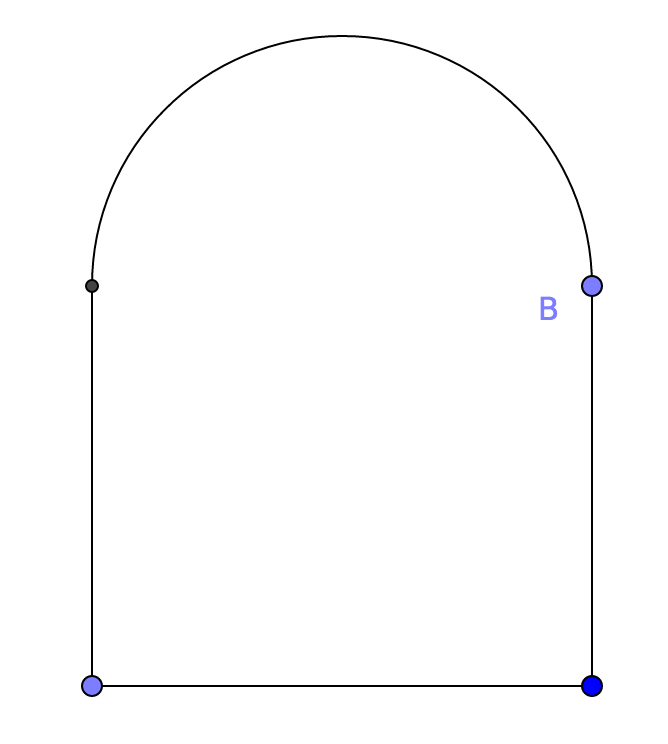
\includegraphics[scale=0.5]{1}
\centering 
\end{figure}

\noindent 3. ?


\newpage
\subsection{} \noindent\fbox{
\parbox{\linewidth}{
Soit $C$ un convexe compact de $\mathbb R^n$. 
\begin{enumerate}
\item Pour $a\in \mathbb R^n\setminus \{0\}$ on considère $\varphi:C\to \mathbb R, x\mapsto 2\langle a,x\rangle$. Montrer que $\varphi$ admet un maximum sur $C$ atteint en un point $x_0$.
\item Soit $H_a=\{x\in \mathbb R^n|\; \langle a,x\rangle=\langle a,x_0\rangle \}$. Montrer que $H_a\cap C$ est un convexe non vide.
\end{enumerate}
}}\\ 
\\ 
\\
\noindent 1. $\varphi$ est continue sur $\mathbb R^n$ (car linéaire à partir d'un espace de dimension finie), donc elle admet un maximum sur le compact $C$.\newline 
2. $H_a$ contient $x_0$. Montrons que $H_a$ est convexe. Soit $x,y\in H_a$ et $\lambda\in [0,1]$. Alors $\langle a,\lambda x +(1-\lambda)y\rangle = \lambda \langle a,x\rangle + (1-\lambda) \langle a,y\rangle = \lambda \langle a,x_0\rangle + (1-\lambda) \langle a,x_0\rangle = \langle a,x_0\rangle$ donc $\lambda x +(1-\lambda)y\in H_a$ et $H_a$ est convexe.\newline 
$H_a\cap C$ est donc convexe comme intersection de deux convexes et non vide car il contient $x_0$.

\subsection{} \noindent\fbox{
\parbox{\linewidth}{
Soient $H$ un espace de Hilbert et $C$ une partie convexe fermée non vide de $H$.
\begin{enumerate}
\item On considère $f:H\to \mathbb R$ définie par $f(x)=(d(x,C))^2$. Montrer que $f$ est différentiable en tout point et calculer la différentielle de $f$ en un point $x$ de $H$. (On considérera le projecteur $P$ de meilleure approximation sur $C$).
\item Soit $\varphi: H\to \mathbb R$ définie par $\varphi(x)=\langle Ax,x\rangle + \langle f,x\rangle$ où $f\in H$ et $A\in \mathcal L_c(H,H)$ auto-adjointe. Déterminer le gradient de $\varphi$ en $x$.
\end{enumerate}
}}\\ 
\\ 
\\
\noindent 1. On rappelle que la projection sur un convexe fermé d'un Hilbert est unique et on notera $p_C(x)$ le projeté de $x$ sur $C$. On rappelle que $p_C$ est $1$-lipschitzienne. \newline
\newline
Soit $x\in H$ fixé et $h\in H$. On a le développement $$\begin{aligned}
\hspace{-2cm}d(x+h,C)^2 &= \|x+h-p_C(x+h)\|^2 \\
&= \|x-p_C(x)+h+p_C(x)-p_C(x+h)\|^2 \\
&= d(x,C)^2+2\langle x-p_C(x),h\rangle + 2\langle x-p_C(x),p_C(x)-p_C(x+h)\rangle + \|p_C(x)-p_C(x+h)+h\|^2\\
&= d(x,C)^2+2\langle x-p_C(x),h\rangle + 2\langle p_C(x)-p_C(x+h),h+x-p_C(x)\rangle + \|p_C(x)-p_C(x+h)\|^2+\|h\|^2
\end{aligned}
$$
Le candidat naturel pour la différentielle de $f$ en $x$ est donc $h\mapsto 2\langle x-p_C(x),h\rangle$.\newline
Sachant que $p_C$ est $1$-lipschitzienne il facile de montrer que $\|p_C(x)-p_C(x+h)\|^2+\|h\|^2 = o(\|h\|)$.\newline \newline
Cependant il est \textbf{remarquablement difficile} de prouver par des moyens élémentaires que $\langle p_C(x)-p_C(x+h),h+x-p_C(x)\rangle = o(\|h\|)$. (On peut montrer facilement que c'est un $O(\|h\|)$ mais c'est insuffisant).\newline 
\newline
On adopte une approche différente:\newline
\textbf{Lemme}: Soit $f,g_1,g_2:H\to \mathbb R$ trois fonctions différentiables en $x\in H$ avec $U$ un voisinage de $x$ et  $$\forall y\in U, g_1(y)\leq f(y)\leq g_2(y)$$ et $g_1(x)=g_2(x)$. \newline  Alors $dg_1(x)=dg_2(x)$, $f$ est différentiable en $x$ et $df(x)=dg_1(x)$.\newline \newline
\underline{Preuve}: Pour $h\in U-x$ on a $g_1(x+h)\leq g_2(x+h)$. On dispose de deux fonctions $\varepsilon_1$ et $\varepsilon_2:H\to \mathbb R$ nulles et continues en $0$ telles que $$g_1(x)+dg_1(x)(h)+\|h\|\varepsilon_1(h)\leq g_2(x)+dg_2(x)(h)+\|h\|\varepsilon_2(h)$$
ie $$dg_2(x)(h) -dg_1(x)(h) + \|h\|(\varepsilon_2(h) -\varepsilon_1(h)) \geq 0$$
Pour $t>0$ on remplace $h$ par $th$ et on obtient 
$$t(dg_2(x)(h) -dg_1(x)(h)) + t\|h\|(\varepsilon_2(th) -\varepsilon_1(th)) \geq 0$$
En simplifiant par $t$ puis en faisant $t\to 0$,
$$dg_2(x)(h) -dg_1(x)(h) \geq 0$$
En remplaçant $h$ par $-h$ dans la dernière inégalité,
$$dg_2(x)(h) -dg_1(x)(h) \leq 0$$
donc $dg_2(x)(h) =dg_1(x)(h)$, ceci étant vrai pour tout $h\in H$, donc $dg_2(x)=dg_1(x)$.\newline \newline
Posons $dg(x):=dg_1(x)$ et réécrivons l'inégalité $g_1(x+h)\leq f(x+h)\leq g_2(x+h)$:
$$f(x)+dg(x)(h)+\|h\|\varepsilon_1(h) \leq f(x+h) \leq f(x)+dg(x)(h)+\|h\|\varepsilon_2(h)$$ 
donc 
$$ \varepsilon_1(h)\leq \frac{f(x+h)-f(x)-dg(x)(h)}{\|h\|}\leq \varepsilon_2(h)$$
Par encadrement, on a pour $\|h\|\to 0$, $\dfrac{f(x+h)-f(x)-dg(x)(h)}{\|h\|}\to 0 $. \newline
\null \hfill $\square$\\

\noindent Revenons au problème. Soit $x\in H\setminus C$ fixé. Posons $x^*=p_C(x)$, $e=\frac{x-x^*}{\|x-x^*\|}$ et $\mathcal H$ l'hyperplan d'appui en $x^*$ de normale $e$, de sorte que $$\mathcal H=\{y\in H, \langle y,e\rangle = \langle x^*,e\rangle\}$$
\textbf{Lemme}: On note $p_{\mathcal H}$ la projection orthogonale sur $\mathcal H$ (qui est un sev fermé). Soit $y\in \mathcal H^+$ et $z\in \mathcal H^-$. Alors $\|y-p_{\mathcal H}(y)\|\leq \|y-z\|$.  \newline \newline
\underline{Preuve}: C'est géométriquement évident (faire un dessin). Formellement, comme 
$\begin{aligned}[t]\|y-z\|^2&=\|y-p_{\mathcal H}(y) + p_{\mathcal H}(y)-z\|^2 \\
&= \|y-p_{\mathcal H}(y)\|^2 + \|p_{\mathcal H}(y)-z\|^2 -2\langle y-p_{\mathcal H}(y), z-p_{\mathcal H}(y)\rangle
\end{aligned}$\newline
il suffit de prouver que $\langle y-p_{\mathcal H}(y), z-p_{\mathcal H}(y)\rangle \leq 0$ (ce qui est encore une évidence géométrique).\newline
Comme $y-p_{\mathcal H}(y)\in \mathcal H^\bot$ (cf théorème de la projection orthogonale sur un sev fermé), et que $\mathcal H^{\bot}=\operatorname{Vect}(e)$ on peut écrire \newline
$y-p_{\mathcal H}(y) = \lambda e$ d'où $\begin{aligned}[t]\langle y-p_{\mathcal H}(y), e\rangle &= \lambda \|e\|^2=\lambda\\ 
&= \langle y, e\rangle - \langle p_{\mathcal H}(y), e\rangle \\
&\geq \langle x^*, e\rangle - \langle p_{\mathcal H}(y), e\rangle \quad \text{car }y\in \mathcal H^+ \\
&= \langle x^*, e\rangle - \langle x^*, e\rangle \quad \text{car }p_{\mathcal H}(y)\in \mathcal H \\
&= 0 \end{aligned} $\newline 
donc $\lambda \geq 0$.\newline
Finalement, $\begin{aligned}[t] \langle y-p_{\mathcal H}(y), z-p_{\mathcal H}(y)\rangle &= \lambda \langle e, z-p_{\mathcal H}(y) \rangle \\
&= \lambda \left( \langle e, z\rangle - \langle e, p_{\mathcal H}(y) \rangle \right)\\
&\leq \lambda \left( \langle e, x^*\rangle - \langle e, x^* \rangle \right) \; \text{car } \lambda\geq 0,\; z\in \mathcal H^-, \;p_{\mathcal H}(y)\in \mathcal H \\
&= 0
\end{aligned}$\newline
comme souhaité. \null \hfill $\square$\\

\noindent Dans notre problème on dispose d'un voisinage de $x$ noté $U$ tel que $U\subset \mathcal H^+$. Pour $y\in U$, comme $p_C(y)\in C\subset \mathcal  H^-$, le lemme donne $(d(y,\mathcal H))^2\leq (d(y,C))^2$. On a aussi la majoration triviale $(d(y,C))^2\leq \|y-x^*\|^2$. En bref $$(d(y,\mathcal H))^2\leq (d(y,C))^2\leq \|y-x^*\|^2$$
Par ailleurs $(d(y,\mathcal H))^2$ se réécrit simplement $$\langle y-p_{\mathcal H}(y),e\rangle^2  = \langle y-x^*,e\rangle^2 = \langle y-x^*,\frac{x-x^*}{\|x-x^*\|}\rangle^2 $$
D'où l'encadrement $$\underbrace{\langle y-x^*,\frac{x-x^*}{\|x-x^*\|}\rangle^2}_{:= g_1(y)}\leq (d(y,C))^2\leq \underbrace{\|y-x^*\|^2}_{:= g_2(y)}$$
On a bien $g_1(x)=g_2(x)$, $g_1$ différentiable en $x$ et $g_2$ différentiable en $x$ de différentielle $h\mapsto 2\langle h,x-x^* \rangle$ (application linéaire continue par Cauchy-Schwarz).\newline
D'après le lemme, $f$ est différentiable en $x$ de différentielle $h\mapsto 2\langle h,x-x^* \rangle$.\newline \newline
Il reste à traiter le cas où $x\in C$. Il suffit de noter qu'alors $$(d(x+h,C))^2\leq \|(x+h)-x\|^2=\|h\|^2$$
Donc $f$ est différentiable de différentielle nulle.\newline \newline
2. Pour $x\in H$ on a le développement 
$$\begin{aligned}
\varphi(x+h) &= \varphi(x) + \langle Ax,h\rangle + \langle Ah,x\rangle + \langle f,h\rangle + \langle Ah,h\rangle\\
&= \varphi(x) + \langle Ax,h\rangle + \langle h,Ax\rangle + \langle f,h\rangle + \langle Ah,h\rangle \quad \text{car }A \text{ auto-adjointe} \\
&= \varphi(x) + \langle h, 2Ax + f\rangle +\langle Ah,h\rangle
\end{aligned}$$
$h\mapsto \langle h, 2Ax + f\rangle$ est linéaire et continue (par Cauchy-Schwarz). Par ailleurs, $$\frac{|\langle Ah,h\rangle|}{\|h\|}\leq \|Ah\|\leq \|A\|_{op}\|h\| \xrightarrow[\|h\|\to 0]{} 0$$
$\varphi$ est donc différentiable en $x$, de gradient $2Ax + f$.

\subsection{} \noindent\fbox{
\parbox{\linewidth}{
Soit $C$ un convexe de $\mathbb R^n$. Pour $0\geq b \geq a$, montrer que $$aC-bC=(a-b)C+b(C-C)$$
}}\\ 
\\ 
\\
\noindent $\subset$ Soit $ac-bc'\in aC-bC$. Alors  $$ac-bc'=(a-b)c+b(c-c')\in (a-b)C+b(C-C)$$ \newline \newline
$\supset$ Soit $(a-b)c+b(c'-c'')\in (a-b)C+b(C-C)$. On a
$$\begin{aligned}
(a-b)c+b(c'-c'') &= -\left( (b-a)c + (-b)(c'-c'') \right) \\
&= -\left( (-a)  \underbrace{\left[\left(1-\frac{b}{a}\right)c + \frac{b}{a}c'\right]}_{\in C}  + bc''\right) \\
&= a \left[\left(1-\frac{b}{a}\right)c + \frac{b}{a}c'\right] - b c''\\
&\in aC - bC
\end{aligned}$$

\subsection{} \noindent\fbox{
\parbox{\linewidth}{
Soit $C$ un fermé de $\mathbb R^n$ tel que $\forall x,y \in C,\; ]x,y[\cap C \neq \emptyset$.\newline
Montrer que $C$ est convexe.
}}\\ 
\\ 
\\
\noindent Supposons par l'absurde que $C$ n'est pas convexe: on dispose alors de $x,y\in C$ et $\alpha\in ]0,1[$ tel que $(1-\alpha)x+\alpha y\notin C$.\newline\newline 
Considérons $\mu=\inf\{\lambda\geq \alpha| (1-\lambda)x+\lambda y\in C\} $ . On dispose de $\lambda_n$ une suite qui décroit vers $\mu$ avec pour tout $n$, $(1-\lambda_n)x+\lambda_n y\in C$ et $\lambda_n\geq \alpha$. En passant à la limite, comme $C$ est fermé, on a $(1-\mu)x+\mu y\in C$ et $\mu\geq \alpha$. Comme $(1-\alpha)x+\alpha y\notin C$, l'inégalité est stricte: $\mu>\alpha$ .\newline \newline
De même, on pose $\nu=\sup\{\lambda\leq \alpha| (1-\lambda)x+\lambda y\in C\} $. On a encore $(1-\nu)x+\nu y\in C$ et $\nu< \alpha$.\newline \newline
Posons $a=(1-\mu)x+\mu y$ et $b=(1-\nu)x+\nu y$. Alors $]a,b[\cap C\neq \emptyset$: on dispose de $\gamma\in ]0,1[$ tel que $(1-\gamma)b+\gamma a\in C$. \newline \newline
Or $(1-\gamma)b+\gamma a = (1-[(1-\gamma)\nu + \gamma \mu])x + [(1-\gamma)\nu + \gamma \mu]y\;$ avec $$(1-\gamma)\nu + \gamma \mu\in \; ]\nu,\mu[ 
$$
Ceci contredit la définition de $\nu$, absurde.

\subsection{} \noindent\fbox{
\parbox{\linewidth}{
Soit $X$ un fermé de $\mathbb R^n$ et $x\in X$. On dit que $v\in \mathbb R^n$ est une direction asymptotique de $X$ en x si $$\forall a\geq 0,\; x+av\in X$$ On note $K(X,x)$ l'ensemble des directions asymptotiques de $X$ en $x$.
\begin{enumerate}
\item Montrer que $\forall x\in X, \; K(X,x)$ est un cône.
\item Si $X$ est convexe, montrer que $K(X,x)$ est convexe et que si $x,x'\in X$, alors $K(X,x)=K(X,x')$.
\end{enumerate}
}}\\ 
\\ 
\\
\noindent 1. Soit $x\in X$, $v\in K(X,x)$ et $\lambda\geq 0$. Montrons que $\lambda v\in K(X,x)$. Pour $a\geq 0$, $a\lambda \geq 0$ donc $x+a\lambda v\in X$, donc $\lambda v\in K(X,x)$.\newline \newline
2. On suppose $X$ convexe. Montrons que $K(X,x)$ est convexe. Pour $v,v'\in K(X,x)$, $\lambda\in [0,1]$ et $a\geq 0$ $$x+a[(1-\lambda)v + \lambda v'] = (1-\lambda)(\underbrace{x+av}_{\in X}) + \lambda(\underbrace{x+av'}_{\in X})\in X$$
Donc $(1-\lambda)v + \lambda v'\in X$ et $K(X,x)$ est convexe.\newline \newline
Soient $x,x'\in X$. Montrons que $K(X,x) \subset K(X,x')$. Soit $v\in K(X,x)$ et $a\geq 0$. On remarque que 
$$ x' + av = \lim_n \left( \underbrace{\left( 1-\frac 1n\right)x' + \frac{1}{n}(\underbrace{x+nav}_{\in X})}_{\in X}\right) $$
Comme $X$ est fermé, $x' + av \in X$ donc $x'\in K(X,x)$ et $K(X,x) \subset K(X,x')$.\newline
On a l'inclusion inverse par symétrie.

\subsection{} \noindent\fbox{
\parbox{\linewidth}{

}}\\ 
\\ 
\\
\noindent

\subsection{} \noindent\fbox{
\parbox{\linewidth}{
Soit $X$ un convexe de $\mathbb R^n$ et $A$ un convexe de $\mathbb R^+$ qui contient $0$. \newline
Montrer que $\bigcup_{a\in A}aX$ est convexe.\newline
}}\\ 
\\ 
\\
\noindent Soient $x,y\in\bigcup_{a\in A}aX $. On dispose de $a,b\in A$ et $x_1,x_2\in X$ tels que $x=ax_1$ et $y=bx_2$. Soit $\lambda \in [0,1]$. \newline
Il s'agit de montrer que $(1-\lambda)a x_1 + \lambda b x_2\in \bigcup_{a\in A}aX$.\newline
\newline
Si $a=0$ ou $b=0$, en supposant par exemple que $a=0$, il suffit de prouver que $\lambda bx_2 \in \bigcup_{a\in A}aX$. Comme $\lambda b = (1-\lambda)0 +\lambda b$, on a $\lambda bx_2\in (\lambda b) X$.\newline \newline
Si $a\neq 0$ et $b\neq 0$, on remarque qu'on a l'égalité
$$ \underbrace{(\lambda a + (1-\lambda)b)}_{\in A} \underbrace{\left[ \left( 1-\frac{(1-\lambda)b }{\lambda a +(1-\lambda)b }\right)x_1 + \frac{(1-\lambda)b }{\lambda a +(1-\lambda)b }x_2 \right]}_{\in C}=(1-\lambda)a x_1 + \lambda b x_2$$
ce qui prouve le résultat.



\subsection{} \noindent\fbox{
\parbox{\linewidth}{
\begin{enumerate}
\item Soit $X$ une partie de $\mathbb R^n$ à $N$ éléments ($N>n+1$). Montrer qu'il est possible de partitionner $X$ en deux parties $X_1$ et $X_2$ tels que $$\co(X_1) \cap \co(X_2) \neq \emptyset$$
\item Soit $(X_i)_{i\in \llbracket 1,N \rrbracket }$ $N$ parties convexes fermées de $\mathbb R^n$ avec $N>n$.\newline
Montrer par récurrence sur $N$ le théorème de Helly: si toute sous-famille de $(X_i)$ à $n+1$ éléments  a une intersection non vide, alors les $N$ convexes de la famille $(X_i)$ sont d'intersection non vide.
\end{enumerate}  
}}\\ 
\\ 
\\
\noindent 1. On adapte facilement la preuve du 4.3 avec $N\geq n+2$ au lieu de $N=n+2$.
\newline \newline
2. On procède par récurrence sur $N\geq n+1$, $n$ étant fixé dans toute la preuve.\newline
L'initialisation est immédiate. Supposons le résultat vrai pour $N-1$ et prouvons le pour $N$. Supposons par l'absurde que toute sous-famille de $(X_i)$ à $n+1$ éléments a une intersection non vide mais que $X_1,\ldots, X_N$ sont d'intersection vide.\newline
D'après l'hypothèse de récurrence appliquée à chaque sous-famille à $N-1$ éléments des $(X_i)$, on dispose pour chaque $i\in \llbracket 1,N \rrbracket$ de $x_i\in \bigcap_{j\neq i} X_j\setminus X_i$.\newline
Posons $A=\{x_1,\ldots,x_N\}$. D'après le résultat du 1., il exise une partition de $A$ en $A_1\cup A_2$ avec $\co(A_1)\cap \co(A_2)\neq \emptyset$.\newline
Considérons $x\in \co(A_1)\cap \co(A_2)$ et montrons que $x\in \bigcap_{i=1}^N X_i$. Soit $i\in \llbracket 1,N \rrbracket$. \newline
Si $x_i\in A_1$, $A_2$ ne contient que des $x_j$ où $j\in \llbracket 1,N \rrbracket\setminus \{i\}$, donc $A_2\subset X_i$. Or $X_i$ est convexe, donc $\co(A_2)\subset X_i$, donc $x\in X_i$. On procède similairement lorsque $x_i\in A_2$.\newline 
Donc $x\in \bigcap_{i=1}^N X_i$ ce qui est absurde.

\subsection{} \noindent\fbox{
\parbox{\linewidth}{
Montrer que l'ensemble suivant est convexe: $$C=\{(a,b,c)\in \mathbb R^3|\; a>0,\; b^2-4ac<0\}$$
}}\\ 
\\ 
\\
\noindent Soient $(a,b,c)$, $(a',b',c')\in C$ et $\lambda \in [0,1]$.\newline
 Il s'agit de montrer que $(1-\lambda)(a,b,c) + \lambda(a',b',c')\in C$.\newline
 Considérons les polynômes $P(X)=aX^2 + bX + c$ et $Q(X)=a'X^2 + b'X + c'$. Comme $(a,b,c)\in C$, $P$ est un polynôme strictement positif, au sens où $$\forall x \in \mathbb R, P(x)>0$$
 De même, $Q$ est strictement positif.\newline \newline
 Or, pour deux réels strictement positifs $x>0$ et $y>0$, on a pour tout $\lambda \in [0,1]$, $(1-\lambda)x +\lambda y>0$. \newline \newline
 On en déduit que $(1-\lambda)P +\lambda Q$ est un polynôme strictement positif dont les coefficients  sont $((1-\lambda)a+\lambda a',(1-\lambda)b+\lambda b',(1-\lambda)c+\lambda c')$.\newline
 Ceci implique $((1-\lambda)a+\lambda a',(1-\lambda)b+\lambda b',(1-\lambda)c+\lambda c')\in C$, soit encore $$(1-\lambda)(a,b,c) + \lambda(a',b',c')\in C$$



\newpage
\section{Fonctions convexes}


\subsection{} \noindent\fbox{
\parbox{\linewidth}{
Soient $E$ un evn et $f:E\to \mathbb R$ convexe et impaire.
\begin{enumerate}
\item Montrer que $\forall x\in E, \; \forall \lambda\in ]0,1[, \; f(\lambda x)\leq \lambda f(x)$.
\item En déduire que $\forall x\in E, \; \forall \lambda\in ]0,1[, \; f(\lambda x) = \lambda f(x)$.
\item En déduire que $f$ est linéaire.
\end{enumerate}
}}\\ 
\\ 
\\
\noindent 1. On note que par imparité $f(0)=f(-0)=-f(0)$ donc $2f(0)=0$ et $f(0)=0$.\newline 
Pour $x\in E$ et $\lambda\in ]0,1[$ on a $$f(\lambda x) =f(\lambda x + (1-\lambda)\cdot 0)\leq \lambda f(x) + (1-\lambda)f(0)=\lambda f(x)$$
2. Pour $x\in E$ et $\lambda\in ]0,1[$, $-f(\lambda x) = f(\lambda (-x)) \leq \lambda f(-x) = -\lambda f(x)$ donc $f(\lambda x)\geq \lambda f(x)$. En combinant avec l'inégalité de 1. on a l'égalité $f(\lambda x)= \lambda f(x)$. \newline \newline
3. Il suffit de prouver que pour $\lambda >1$, $f(\lambda x)=\lambda f(x)$.\newline
On remarque que pour $\lambda >1$, $\frac 1 \lambda <1$ et $$\begin{aligned}
f(\frac 1 \lambda (\lambda x) ) &= \frac 1 \lambda f(\lambda x)\\
\implies f(\lambda x) &= \lambda f(x)
\end{aligned}$$
comme souhaité.


\subsection{} \noindent\fbox{
\parbox{\linewidth}{
Soit $f>0$ positivement homogène sur $C$ convexe. Montrer que $f$ est convexe si et seulement si $B=\{x\in C|\; f(x)\leq 1\}$ est convexe.
}}\\ 
\\ 
\\
\noindent Pour que $f$ soit homogène, il faut pouvoir définir $f(\lambda x)$ pour tout $\lambda \geq 0$, ce qui nécessite une structure additionnelle sur $C$. On supposera donc que $C$ est un $\mathbb R$-evn. Par positivement homogène l'énoncé veut dire homogène de degré 1.\newline \newline
$\impliedby$ Supposons $B$ convexe et montrons que $\epi f$ est convexe. On rappelle que $$\epi f= \{(x,y)\in C\times \mathbb R|\;y\geq f(x)\}$$
Soient $(x_1,y_1)$, $(x_2,y_2)$ dans $\epi f$ et $\lambda \in [0,1]$. $f$ étant homogène de degré $1$ et strictement positive, les inégalités $y_1\geq f(x_1)>0$ et $y_2\geq f(x_2)>0$ se réécrivent $1\geq f(\frac{1}{y_1}x_1)$ et $1\geq f(\frac{1}{y_2}x_2)$ donc $\frac{x_1}{y_1}$ et $\frac{x_2}{y_2}$ sont dans $B$.\newline \newline 
$B$ étant convexe et $\dfrac{\lambda y_2}{(1-\lambda)y_1 + \lambda y_2}$ étant dans $[0,1]$, on a $$f\left(\left(1-\dfrac{\lambda y_2}{(1-\lambda)y_1 + \lambda y_2}\right)\frac{x_1}{y_1} + \dfrac{\lambda y_2}{(1-\lambda)y_1 + \lambda y_2}\frac{x_2}{y_2}\right)\leq 1$$
ce qui se réécrit $$f((1-\lambda)x_1 + \lambda x_2)\leq (1-\lambda)y_1 + \lambda y_2$$
ce qui équivaut à $((1-\lambda)x_1 + \lambda x_2,(1-\lambda)y_1 + \lambda y_2)\in \epi f$.\newline
Donc $\epi f$ est convexe, donc $f$ est convexe.\newline 
\newline 
$\implies$ On suppose $f$ convexe. Montrons que $B$ est convexe.\newline
Soit $x,y\in C$ tel que $f(x)\leq 1$ et $f(y)\leq 1$ et $\lambda \in [0,1]$. Alors $$f((1-\lambda)x+\lambda y)\leq (1-\lambda)f(x) + \lambda f(y)\leq 1$$
Donc $B$ convexe.

\subsection{} \noindent\fbox{
\parbox{\linewidth}{

}}\\ 
\\ 
\\
\noindent 

\subsection{} \noindent\fbox{
\parbox{\linewidth}{
Soient $x_i>0$, $\alpha_i\geq 0$ et $\sum_{i=1}^n\alpha_i =1$. Montrer que $$\sum_{i=1}^n\alpha_i x_i \geq \prod_{i=1}
^nx_i^{\alpha_i}$$
}}\\ 
\\ 
\\
\noindent Par concavité du $\log$ et l'inégalité de Jensen on a $$\ln\left( \sum_{i=1}^n\alpha_i x_i \right)\geq \sum_{i=1}^n \alpha_i \ln(x_i)$$
et on a l'inégalité voulue en passant à l'exponentielle.

\subsection{} \noindent\fbox{
\parbox{\linewidth}{
Soit $I$ un intervalle contenu dans $\mathbb R^*_+$ et $f:\mathbb R^+\to \mathbb R$ $2$ fois dérivable.\newline
Montrer que si $g:x\mapsto f(\frac{1}{x})$ est convexe dans $I$, alors $h:x\mapsto xf(x)$ est aussi convexe et réciproquement.
}}\\ 
\\ 
\\
\noindent Il me semble nécessaire d'ajouter l'hypothèse $x\in I \implies \frac{1}{x}\in I$.\newline \newline
On note que $$g''(x) = \frac{f''(\frac{1}{x}) + 2xf'(\frac{1}{x})}{x^4}$$
donc 
$$g''(\frac{1}{x}) = x^3 (xf''(x)+2f'(x)) = x^3 h''(x)$$
Pour $x\in I$, $g''(\frac{1}{x})$ et $h''(x)$ ont donc même signe. $g$ est donc convexe si et seulement si $h$ l'est.

\subsection{} \noindent\fbox{
\parbox{\linewidth}{
Soit $f:[a,b]\to \mathbb R$ bornée.\newline
On définit $\varphi: \mathbb R\to \mathbb R$ par $\varphi(t)=\inf_{x\in [a,b]}(-xt-f(x))$\newline
Montrer que $\varphi$ est concave.
}}\\ 
\\ 
\\
\noindent Montrons que $\psi:t\mapsto \sup_{x\in [a,b]}(xt + f(x))$ est convexe.\newline
Soient $t,t' \in \mathbb R$ et $\lambda \in [0,1]$. Pour $x\in [a,b]$, $xt+f(x)\leq \psi(t)$ et $xt'+f(x)\leq \psi(t')$ donc $$ \begin{aligned}(1-\lambda)(xt+f(x)) + \lambda(xt'+f(x)) &\leq (1-\lambda) \psi(t) + \lambda \psi(t')\\
x((1-\lambda)t + \lambda t') + f(x)&\leq (1-\lambda) \psi(t) + \lambda \psi(t') \end{aligned}$$
ceci étant vrai pour tout $x\in [a,b]$. En passant au $\sup$ on obtient $$\psi((1-\lambda)t + \lambda t')\leq (1-\lambda) \psi(t) + \lambda \psi(t')$$
$\psi$ est donc convexe, donc $\varphi=-\psi$ est concave.

\subsection{} \noindent\fbox{
\parbox{\linewidth}{
Soient $t\in [a,b]$, $x\in \mathbb R^n$ et $f:\mathbb R^n\times [a,b] \to \mathbb R, (x,t)\to f(x,t)$ telle que\newline
$f$ est convexe en $x$ et continue en $t$.\newline
Montrer que $g:x\mapsto \int_a^bf(x,t) dt$ est convexe.
}}\\ 
\\ 
\\
\noindent Soient $x,y\in \mathbb R^n$ et $\lambda \in [0,1]$. Pour $t\in [a,b]$, par convexité de $f$ en la première variable, $f((1-\lambda)x+\lambda y,t)\leq (1-\lambda)f(x,t) + \lambda f(y,t)$.\newline
En intégrant cette inégalité selon $t$ on trouve $$g((1-\lambda)x+\lambda y)\leq (1-\lambda)g(x) + \lambda g(y)$$ donc $g$ est convexe.

\subsection{} \noindent\fbox{
\parbox{\linewidth}{
Soit $A$ une partie fermée non vide d'un evn $E$.\newline 
Montrer que $A$ est convexe si et seulement si $x\mapsto d(A,x)$ est convexe de $E$ dans $\mathbb R$.
}}\\ 
\\ 
\\
\noindent $\implies$ Supposons $A$ convexe et montrons que $x\mapsto d(A,x)$ est convexe. Soient $x,y\in E$ et $\lambda\in ]0,1[$.\newline
Soit $x',y'$ deux éléments quelconques de $A$. On a l'inégalité $$(1-\lambda)\|x-x'\| + \lambda \|y-y'\|\geq \|(1-\lambda)x+\lambda y- \underbrace{(	(1-\lambda)x'+\lambda y')}_{\in A}\|\geq d(A, (1-\lambda)x+\lambda y)$$ 
donc $$\|x-x'\| \geq \frac{1}{1-\lambda } (d(A, (1-\lambda)x+\lambda y) -\lambda \|y-y'\|)$$
Le membre de droite est indépendant de $x'$, donc au passant à l'inf sur $x'$ on a
$$d(A,x)\geq \frac{1}{1-\lambda } (d(A, (1-\lambda)x+\lambda y) -\lambda \|y-y'\|) $$
soit encore $$ (1-\lambda )d(A,x)\geq  d(A, (1-\lambda)x+\lambda y) -\lambda \|y-y'\|$$
qui devient $$ \lambda \|y-y'\| \geq d(A, (1-\lambda)x+\lambda y) - (1-\lambda )d(A,x)$$
Un raisonnement similaire (passage à l'inf sur $y'$) donne 
$$\lambda d(A,y) \geq d(A, (1-\lambda)x+\lambda y) - (1-\lambda )d(A,x)$$
soit $$ d(A, (1-\lambda)x+\lambda y) \leq (1-\lambda )d(A,x) + \lambda d(A,y)$$
Donc $x\mapsto d(A,x)$ est convexe.\newline
\newline 
$\impliedby$ On suppose que $x\mapsto d(A,x)$ est convexe. Soient $x,y\in A$ et $\lambda\in [0,1]$. \newline
On a $d(A,(1-\lambda)x+\lambda y)\leq (1-\lambda)d(A,x) + \lambda d(A,y) = (1-\lambda)\cdot 0+ \lambda \cdot 0 = 0$.\newline
Donc $d(A,(1-\lambda)x+\lambda y)=0$ et comme $A$ est fermé, $(1-\lambda)x+\lambda y\in A$, donc $A$ convexe.

\subsection{} \noindent\fbox{
\parbox{\linewidth}{
Soit $f_n:\;]0,1[\to \mathbb R$ une suite de fonctions convexes qui converge simplement vers $f:\; ]0,1[\to \mathbb R$.
\begin{enumerate}
\item Montrer que $f$ est convexe.
\item Montrer que $f_n$ converge vers $f$ uniformément sur tout compact de $]0,1[$.
\end{enumerate}
}}\\ 
\\ 
\\
\noindent 1. Soient $x,y\in ]0,1[$ et $\lambda\in [0,1]$. Pour tout $n$, $$f_n((1-\lambda)x+\lambda y)\leq (1-\lambda)f_n(x) + \lambda f_n(y)$$ et en passant à la limite sur $n$ on a la convexité de $f$.\newline \newline
2. Etant donné $K$ un compact de $]0,1[$, montrons que la famille des $(f_n)$ est uniformément lipschitzienne, c'est-à-dire qu'il existe $A\geq 0$ tel que $$\forall n\geq 1,\; \forall x,y\in K,\quad |f_n(x)-f_n(y)|\leq A |x-y|$$
$K$ étant compact il est inclus dans un segment $[a,b]$ avec $0<a<b<1$. Considérons $c<c'\in ]0,a[$ et $d<d'\in ]b,1[$.\newline
Soient $x,y\in K$ et $n\geq 1$ quelconques. Par convexité de $f$, $$\frac{f_n(c')-f_n(c)}{c'-c} \leq \frac{f_n(y)-f_n(x)}{y-x}\leq \frac{f_n(d')-f_n(d)}{d'-d}$$
$\left(\frac{f_n(c')-f_n(c)}{c'-c}\right)_n$ et $\left(\frac{f_n(d')-f_n(d)}{d'-d}\right)_n$ convergent, donc sont bornées. On dispose donc de $m$ et $M$ des réels tels que $$m\leq \frac{f_n(c')-f_n(c)}{c'-c} \leq \frac{f_n(y)-f_n(x)}{y-x}\leq \frac{f_n(d')-f_n(d)}{d'-d}\leq M$$
Pour tout $n\geq 1$ et $x,y\in K$ on a donc $$ m \leq \frac{f_n(y)-f_n(x)}{y-x} \leq M$$
En posant $A=\max(|m|,|M|)$ on a $$\forall n\geq 1,\; \forall x,y\in K,\quad |f_n(x)-f_n(y)|\leq A |x-y|$$
\null \hfill $\square$ \newline
En passant à la limite sur $n$ dans l'inégalité précédente, on montre facilement que $f$ est $A$-lipschitzienne.\newline
Montrons que $f_n$ converge vers $f$ uniformément sur $K$.\newline
Soit $\varepsilon >0$. \newline
Posons $N=\lfloor \frac{3A}{\varepsilon}\rfloor +1$ et $x_k=\frac{k}{N}$ pour $k\in \llbracket 1,N-1\rrbracket$.\newline
Par convergence simple des $f_n$ on dispose de $N'$ tel que $$n\geq N'\implies \forall k\in \llbracket 1,N-1\rrbracket, |f(x_k)-f_n(x_k)|\leq \frac{\varepsilon}{3}$$
Posons $N''=\max(N,N')$ et considérons $n\geq N''$ et $x\in K$.\newline
Par construction il existe $i\in \llbracket 1,N-1\rrbracket$ tel que $|x-x_i|\leq \frac{\varepsilon}{3A}$, de sorte que 
$$\begin{aligned}
|f(x)-f_n(x)|&\leq |f(x)-f(x_i)| + |f(x_i)-f_n(x_i)| + |f_n(x_i)-f_n(x)| \\
&\leq A |x-x_i| + \frac{\varepsilon}{3}  + A |x-x_i|\\
&\leq \epsilon
\end{aligned}$$
On a donc montré que $\forall n\geq N'',\; \forall x\in K, \; |f(x)-f_n(x)|\leq \epsilon$, d'où la convergence uniforme.


\subsection{} \noindent\fbox{
\parbox{\linewidth}{
Soit $f_1,\ldots, f_n$ des fonctions convexes de $[a,b]$ dans $\mathbb R$ et $g:\mathbb R^n \to \mathbb R$, convexe et croissante en chaque variable.\newline
Montrer que $F:x\mapsto g(f_1(x),\ldots,f_n(x))$ est convexe sur $[a,b]$.
}}\\ 
\\ 
\\
\noindent Soient $x,y\in [a,b]$ et $\lambda\in [0,1]$. On a $$F((1-\lambda)x + \lambda y)=g(f_1((1-\lambda)x + \lambda y),\ldots, f_n((1-\lambda)x + \lambda y))) $$
La convexité de chaque $f_i$ et la croissance de $g$ en chaque argument donne $$\begin{aligned}F((1-\lambda)x + \lambda y)&\leq g((1-\lambda)f_1(x) + \lambda f_1(y),\ldots,(1-\lambda)f_n(x) + \lambda f_n(y)) \\
&=g((1-\lambda) (f_1,(x),\ldots, f_n(x)) + \lambda (f_1,(y),\ldots, f_n(y)) )\\
&\leq (1-\lambda) g(f_1,(x),\ldots, f_n(x)) + \lambda g(f_1,(y),\ldots, f_n(y)) \quad \text{par convexité de } g\\
&= (1-\lambda) F(x) + \lambda F(y)
\end{aligned}
$$
Donc $F$ convexe.

\subsection{} \noindent\fbox{
\parbox{\linewidth}{
Soit $n\geq 1$ et $f:(\mathbb R^*_+)^n\to \mathbb R$ définie par $$f(x_1,\ldots, x_n)=\left(\prod_{i=1}^n x_i \right) ^{1/n}$$
Montrer que $f$ est concave.
}}\\ 
\\ 
\\
\noindent $f$ admet clairement des dérivées partielles à l'ordre $1$ données par $$\frac{\partial f}{\partial x_i}(x_1,\ldots,x_n)=\left( \prod_{j\neq i} x_j\right)^{1/n}\frac{1}{n}\cdot x_i^{ 1/n -1}=\frac{1}{n}\frac{f(x_1,\ldots,x_n)}{x_i}$$
$f$ admet alors clairement des dérivées partielles d'ordre $2$ données par 
$$\frac{\partial^2 f}{\partial x_j \partial x_i}(x_1,\ldots, x_n) = \begin{cases}
\frac{f(x_1,\ldots,x_n)}{n^2} \frac 1{x_i x_j} &\text {si }i\neq j \\
-\frac{n-1}{n^2}f(x_1,\ldots,x_n)\frac{1}{x_i^2} &\text {si } i=j
\end{cases}$$
Chacune de ces fonctions est clairement continue, donc $f$ est $C^2$.\newline
Soit $(x_1\ldots,x_n)\in \mathbb R^n$ fixé dans la suite. La Hessienne de $f$ en $(x_1,\ldots, x_n)$ est donnée par 

\[
   H(f)(x_1,\ldots,x_n) = \frac{f(x_1,\ldots, x_n)}{n^2} \left(
    \begin{array}{ccccc}
    -\frac{n-1}{x_1^2}                                    \\
      & \ddots             &   & \frac{1}{x_i x_j}\\
      &               & \ddots                \\
      & \frac{1}{x_i x_j} &   & \ddots            \\
      &               &   &   & -\frac{n-1}{x_n^2}
    \end{array}
    \right)
\]  
En posant $y=\begin{pmatrix}
\frac 1{x_1}\\
\vdots\\
\frac 1{x_n}
\end{pmatrix}$ et $J=\begin{pmatrix}
\frac 1{x_1^2} \\
& \ddots \\
&& \frac 1{x_n^2}
\end{pmatrix}=\diag(\frac 1{x_1^2},\ldots,\frac 1{x_n^2})$ \newline
on réécrit simplement $$H(f)(x_1\ldots,x_n)=\underbrace{\frac{f(x_1,\ldots, x_n)}{n^2}}_{\text{constante positive}}(yy^T-nJ)$$
Il suffit de prouver que $yy^T-nJ$ est semi-définie négative. Considérons $v\in \mathbb R^n$.
On a $$\begin{aligned}
v^T(yy^T-nJ)v &= (y^Tv)^Ty^Tv-nv^TJv\\
&= \left(\sum_{i=1}^n \frac{v_i}{x_i}\right)^2 - n \sum_{i=1}^n \frac{v_i^2}{x_i^2}
\end{aligned}$$
Or, par Cauchy-Schwarz dans $\mathbb R^n$ muni du produit scalaire euclidien canonique,
$$\begin{aligned} \sum_{i=1}^n \frac{v_i}{x_i} &= \sum_{i=1}^n 1\cdot \frac{v_i}{x_i}\\
&\leq \sqrt{\sum_{i=1}^n 1} \cdot \sqrt{\sum_{i=1}^n \frac{v_i^2}{x_i^2}}
\end{aligned}$$
En passant au carré on obtient $$\left(\sum_{i=1}^n \frac{v_i}{x_i}\right)^2 - n \sum_{i=1}^n \frac{v_i^2}{x_i^2}\leq 0$$ donc $$v^T(yy^T-nJ)v\leq 0$$ d'où $H(f)(x_1,\ldots,x_n)$ semi-définie négative, et ceci pour tout $(x_1,\ldots,x_n)\in (\mathbb R^*_+)^n $ donc $f$ concave.


\subsection{} \noindent\fbox{
\parbox{\linewidth}{
Soit $f:\mathbb R^2\to \mathbb R, (x,y)\mapsto x^2+y^2+xy$.
\begin{enumerate}
\item Montrer que $f$ est convexe.
\item On pose $x=r\cos(\alpha)$ et $y=r\sin(\alpha)$.\newline
Exprimer $\frac{\partial f}{\partial x}$ et $\frac{\partial f}{\partial y}$ en fonction de $\frac{\partial f}{\partial r}$ et $\frac{\partial f}{\partial \alpha}$
\end{enumerate}
}}\\ 
\\ 
\\
\noindent 1. $f$ est $C^2$ de Hessienne $$H(f)(x,y)=\begin{pmatrix}
2 & 1\\
1 & 2
\end{pmatrix}$$
Son déterminant est $3$, les deux valeurs propres sont donc de même signe et non nulles. Sa trace est $4$, les deux valeurs propres sont donc strictement positives. Donc $H(f)(x,y)$ est symétrique définie positive, et ceci pour tout $(x,y)\in \mathbb R^2$ donc $f$ est convexe.\newline
\newline 
2. Avec la formule de calcul des dérivées partielles d'une composée, $$\frac{\partial f}{\partial r} = \cos(\alpha)\frac{\partial f}{\partial x} + \sin(\alpha)\frac{\partial f}{\partial y}$$
et 
$$\frac{\partial f}{\partial \alpha} = -r\sin(\alpha)\frac{\partial f}{\partial x} + r\cos(\alpha)\frac{\partial f}{\partial y}$$


\subsection{} \noindent\fbox{
\parbox{\linewidth}{
Pour $x>0$ et $y>1$ on pose $F(x,y)=x^\alpha (\ln y)^\beta$ où $\alpha$ et $\beta$ sont deux paramètres donnés.
\begin{enumerate}
\item Calculer les dérivées partielles d'ordre $1$ et $2$ de $F$.
\item Montrer que si $F$ est concave alors $\alpha \in [0,1]$ et $\beta \geq 0$.
\item Montrer que si $\alpha \in [0,1]$ et $\beta \geq 0$ alors $F$ est concave sur l'ensemble $$C=\{(x,y)\in \mathbb R^2, \; x>0 \text{ et } \ln y > \frac{\beta}{1-\alpha}-1 \}$$
\item Plus généralement, pour $I$ et $J$ deux intervalles ouverts de $\mathbb R$, $f\in C^2(I,\mathbb R)$ et $g\in C^2(J,\mathbb R)$ on considère $$F:I\times J \to \mathbb R, (x,y)\mapsto f(x)g(y)$$
\begin{enumerate}
\item Montrer que si $F$ est concave avec $f>0$ et $g>0$ alors $f$ et $g$ sont concaves.
\item Montrer que si $f>0$, $g>0$ avec $f^2$ et $g^2$ concaves, alors $F$ est concave.
\end{enumerate}
\end{enumerate}
}}\\ 
\\ 
\\
\noindent 1. $F$ est clairement $C^2$, de dérivées partielles 
$$\begin{aligned}
\frac{\partial f}{\partial x}(x,y) &= \alpha x^{\alpha -1}(\ln y)^\beta\\
\frac{\partial f}{\partial y}(x,y) &= \beta \frac{x^\alpha (\ln y)^{\beta-1} }{y} \\
\frac{\partial^2 f}{\partial^2 x}(x,y) &= \alpha (\alpha -1) x^{\alpha -2}(\ln y)^\beta \\
\frac{\partial^2 f}{\partial y \partial x}(x,y) = \frac{\partial^2 f}{\partial x \partial y}(x,y) &= \alpha \beta \frac{x^{\alpha-1} (\ln y)^{\beta-1} }{y}\\
\frac{\partial^2 f}{\partial^2 y}(x,y) &= \frac{\beta x^\alpha (\ln y)^{\beta-2}}{y^2}(\beta -1 -\ln y)
\end{aligned}$$
La Hessienne de $F$ en $(x,y)$ s'écrit donc 
$$ H(F)(x,y) = \underbrace{x^{\alpha -2}(\ln y)^{\beta-2}}_{\text{constante positive}} \begin{pmatrix}
\alpha(\alpha -1)(\ln y)^2 & \frac{\alpha \beta x\ln y}{y} \\
\frac{\alpha \beta x\ln y}{y} & \frac{\beta x^2}{y^2}(\beta -1 -\ln y)
\end{pmatrix}$$
2. On suppose $F$ concave, donc $H(F)(x,y)$ est semi-définie négative pour tout $(x,y)$. Comme $x^{\alpha -2}(\ln y)^{\beta-2}$ est une constante positive, la matrice $$\begin{pmatrix}
\alpha(\alpha -1)(\ln y)^2 & \frac{\alpha \beta x\ln y}{y} \\
\frac{\alpha \beta x\ln y}{y} & \frac{\beta x^2}{y^2}(\beta -1 -\ln y)
\end{pmatrix}$$
est semi-définie négative.\newline
Son déterminant, qui est donc $\geq 0$, vaut $$\frac{\alpha \beta x^{2 } (\ln y)^2 ((1-\alpha)\ln y +1 -\alpha-\beta)}{y^2}$$
Ceci implique $\forall y>1,\; \alpha \beta ((1-\alpha)\ln y +1 -\alpha-\beta) \geq 0 $\newline
Par des considérations asymptotiques, le facteur devant le $\log$ doit être $\geq 0$ ie  $\alpha \beta (1-\alpha) \geq 0$. \newline 
\newline
On a aussi $$(1,0)\cdot \begin{pmatrix}
\alpha(\alpha -1)(\ln y)^2 & \frac{\alpha \beta x\ln y}{y} \\
\frac{\alpha \beta x\ln y}{y} & \frac{\beta x^2}{y^2}(\beta -1 -\ln y)
\end{pmatrix} \cdot\begin{pmatrix}
1\\ 0
\end{pmatrix}\leq 0$$
qui s'écrit $\alpha(\alpha-1)(\ln y)^2\leq 0$, donc $\alpha(\alpha-1)\leq 0$, donc $\alpha \in [0,1]$.\newline
Par ailleurs, l'inégalité $\alpha \beta (1-\alpha) \geq 0$ devient $\beta \geq 0$. \newline
\newline
3. On suppose $\alpha \in [0,1]$ et $\beta \geq 0$. Montrons que $F$ est concave sur $C$. Comme $C$ est un convexe ouvert, il suffit de montrer que $H(F)(x,y)$ est semi-définie négative pour tout $(x,y)$ dans $C$.\newline 
On rappelle le lemme très pratique en dimension 2:\newline
\textbf{Lemme}:(Conditions de Monge) \newline 
Soit $A=\begin{pmatrix}
r & s\\
s & t
\end{pmatrix}$ une matrice symétrique.\newline
Si $rt-s^2\geq 0$ et $r\geq 0$ alors $A$ est semi-définie positive.\newline
Si $rt-s^2\geq 0$ et $r\leq 0$ alors $A$ est semi-définie négative.\newline \newline
\underline{Preuve}: $A$ étant symétrique , elle est semblable à $D=\begin{pmatrix}
\lambda_1 & 0\\
0 & \lambda_2
\end{pmatrix}$. La condition $rt-s^2\geq 0$ est équivalente à $\det A\geq 0$, ie $\lambda_1 \lambda_2\geq 0$ donc $\lambda_1$ et $\lambda_2$ de même signe. On a par ailleurs $rt\geq s^2\geq 0$ donc $r$ et $t$ ont même signe. Or $\Tr(A)=r+t=\lambda_1 + \lambda_2$. Le signe de $\lambda_1$ est donc celui de $r$ ce qui achève la preuve. \newline
\newline
Dans notre cas, la condition $\ln y > \frac{\beta}{1-\alpha}-1$ implique $(1-\alpha)\ln y + 1-\alpha - \beta >0$, donc $\alpha \beta ((1-\alpha)\ln y + 1-\alpha - \beta) \geq 0$ d'où $\det (H(F)(x,y)) \geq 0$ pour tout $(x,y)\in C$.\newline
Enfin, $H(F)(x,y)_{11} = x^{\alpha -2}(\ln y)^{\beta-2}\alpha\underbrace{(\alpha -1)}_{\leq 0}(\ln y)^2\leq 0$ et d'après le lemme, $H(F)(x,y)$ est semi-définie négative. \newline 
\newline 
4. a) On suppose $F$ concave. On a $$H(F)(x,y) = \begin{pmatrix}
f''(x)g(y) & f'(x)g'(y) \\
f'(x)g'(y) & f(x)g''(y)
\end{pmatrix}$$
Comme $H(F)(x,y)$ est semi-définie négative, $$(1,0)\cdot H(F)(x,y) \begin{pmatrix}
1 \\0
\end{pmatrix} \leq 0$$
ie $f''(x)g(y)\leq 0$. Comme $g>0$, $f''(x)\leq 0$ et ceci pour tout $x\in I$. Donc $f$ concave.\newline
De même on prouve que $g$ est concave.\newline 
\newline
b) $f^2$ et $g^2$ étant concaves et $C^2$ sur des intervalles ouverts, on a $(f^2)''=2(f'^2+ff'')\leq 0$ ie $0\leq f'^2\leq ff'' $ et $0\leq g'^2\leq gg'' $
En multipliant ces deux dernières inégalités entre elles on a $$\forall(x,y)\in I\times J,\; (f''(x)g(y))(f(x)g''(y))\geq (f'(x)g'(y))^2$$
ie $\det(H(F)(x,y))\geq 0$.\newline
Par ailleurs, $f'^2(x)\leq f(x)f''(x)$ implique $f(x)f''(x)\leq -f'^2(x)\leq 0 $ et comme $f>0$, on a $f''(x)\leq 0$. Donc $$H(F)(x,y)_{11}=f''(x)g(y)\leq 0 \quad \text{car } g>0$$
D'après le lemme, $H(F)(x,y)$ est semi-définie négative, et ceci pour tout $(x,y)\in I\times J$ (qui est un ouvert convexe), donc $F$ est concave sur $I\times J$.

\subsection{} \noindent\fbox{
\parbox{\linewidth}{
Soient $f:\mathbb R \to \mathbb R$ convexe et $\varphi:\mathbb R\to \mathbb R^+$.
\begin{enumerate}
\item $\varphi$ étant à support compact, montrer que $F:x\mapsto \int_{-\infty}^{\infty} f(x-t)\varphi(t)dt$ est convexe.
\item On suppose $f>0$ croissante et $C^1$ sur $[a,b]$.\newline
Montrer que l'on peut prolonger $f$ à $]\text{-}\infty, b]$ de manière à ce que la fonction prolongée soit encore convexe, croissante, strictement positive, $C^1$, et constante sur un intervalle de la forme $]\text{-}\infty, \alpha]$.
\item Soient $f,g$ convexes, strictement positives, croissantes et $\mathbb C^1$ sur $[a,b]$. Montrer que $fg$ est convexe sur $[a,b]$.
\end{enumerate} 
}}\\ 
\\ 
\\
\noindent 1. Soient $x,y\in \mathbb R$ et $\lambda \in [0,1]$. Pour $t\in \mathbb R$ on a par convexité de $f$, $$f((1-\lambda)x + \lambda y -t)=f((1-\lambda)(x-t) + \lambda(y-t))\leq (1-\lambda)f(x-t) + \lambda f(y-t)$$
En intégrant cette inégalité suivant $t$ on obtient le résultat voulu.\newline \newline
2. \hfill \textit{Correction proposée par Yannick Guyonvarch}\newline
On définit pour tout $y$
\begin{align*}
    &f_+'(y)=\lim_{x\to y,x\geq y}\frac{f(x)-f(y)}{x-y} \\
    &f_-'(y)=\lim_{x\to y,x\leq y}\frac{f(x)-f(y)}{x-y}
\end{align*}\newline 
Si $f_+'(a)=0$, le résultat est immédiat car en posant $f(x)=f(a)$ pour tout $x\in]-\infty,a]$ on a construit un prolongement $C^1$ de $f$ qui vérifie toutes les contraintes du problème.\newline \newline
Nous nous intéressons donc au cas où $f_+'(a)>0$. Posons $g:x\mapsto e(x-\alpha)^2+d$ avec $\alpha<a$ le point à déterminer tel que pour tout $x\leq\alpha$, on prolonge f par $h:x\mapsto g(\alpha)=d$. Nous devons donc trouver un triplet $(e,\alpha,d)$ qui satisfait au contraintes du problème, à savoir
\begin{align*}
    g\text{ croissante et $C^1$,}\quad g'(\alpha)=0,\quad g'(a)=f'(a),\quad 0<g(\alpha)<f(a),\quad g(a)=f(a),\quad \alpha<a
\end{align*}
\newline
$g$ est bien $C^1$ et $g'(\alpha)=0$. Par ailleurs
\begin{align*}
    &g'(a)=f'(a)\iff2e(a-\alpha)=f'(a)\iff e=\frac{f'(a)}{2(a-\alpha)} \\
    &g(a)=f(a)\iff e(a-\alpha)^2+d=f(a)\iff d=f(a)-\frac{f'(a)(a-\alpha)}{2}
\end{align*}
\newline \newline
$e$ respecte la contrainte $e>0$ (pour avoir $g$ croissante) dès que $\alpha<a$. De la même manière $d<f(a)$ à la même condition.
\newline \newline
Trouvons $\alpha<a$ tel que $0<d$
\begin{align*}
    d>0\iff\alpha>a-\frac{2f(a)}{f'(a)}
\end{align*}
\newline
Ainsi en prenant $\alpha\in]a-\frac{2f(a)}{f'(a)},a[$ on a bien construit un prolongement $C^1$ de $f$ qui vérifie toutes les conditions.\newline
\newline 
3. \hfill \textit{Correction proposée par Yannick Guyonvarch}\newline
Pour tout $x\in[a,b]$, $f(x)g(x)>0$ et $h:x\mapsto f(x)g(x)$ admet une dérivée $h'(x)=f'(x)g(x)+f(x)g'(x)$.
\newline
Soit $x_1\leq x_2$.
\begin{align*}
    h'(x_1)&=f'(x_1)g(x_1)+f(x_1)g'(x_1) \\
    &\leq f'(x_1)g(x_2)+f(x_2)g'(x_1)\text{ car $f$ et $g$ sont croissantes} \\
    &\leq f'(x_2)g(x_2)+f(x_2)g'(x_2)\text{ car $f$ et $g$ de dérivée croissante}\\
    &= h'(x_2)
\end{align*}
\newline
$h'$ est donc croissante sur $[a,b]$ donc $f\times g$ est convexe sur $[a,b]$.



\subsection{} \noindent\fbox{
\parbox{\linewidth}{
Soit $K$ un convexe fermé de $\mathbb R^n$ et $P$ la projection sur $K$.\newline
Montrer que $\varphi:x\mapsto \|x-P(x)\|$ est convexe.
}}\\ 
\\ 
\\
\noindent Soient $x,y\in K$ et $\lambda \in [0,1]$.\newline
Comme $K$ est convexe, $(1-\lambda)P(x) + \lambda P(y)\in K$, donc par définition de $P$,
$$\begin{aligned}\varphi((1-\lambda)x  + \lambda y) &= \|(1-\lambda)x  + \lambda y - P((1-\lambda)x  + \lambda y)\| \\
&\leq \|(1-\lambda)x  + \lambda y - [(1-\lambda)P(x) + \lambda P(y)] \| \\
&= \| (1-\lambda)(x-P(x)) + \lambda (y-P(y))\| \\
&\leq (1-\lambda) \|x-P(x)\| + \lambda \|y-P(y)\| \\
&= (1-\lambda) \varphi(x) + \lambda \varphi(y)
\end{aligned}$$
Donc $\varphi$ convexe.



\subsection{} \noindent\fbox{
\parbox{\linewidth}{
Soient $f,g:\mathbb R^*_+\to \mathbb R$ définies par $f(x,y)=x^\alpha + y^\beta$ et $g(x,y)=x^{\alpha}y^{\beta}$\newline
Etudier la concavité et la convexité de $f$ et $g$.
}}\\ 
\\ 
\\
\noindent $f$ est clairement $C^2$ de Hessienne $H(f)(x,y)=\begin{pmatrix}
\alpha(\alpha-1)x^{\alpha-2} & 0 \\
0 & \beta(\beta-1)y^{\beta-2}
\end{pmatrix}$\newline
Cette matrice est diagonale.\newline
\setlength{\tabcolsep}{0.1em}
\begin{tabular}{ccl}
$f$ est concave & $\iff$ & $H(f)(x,y)$ semi-définie négative pour tout $(x,y)$\\
& $\iff $ & $\alpha(\alpha-1)\leq 0$ et $\beta(\beta-1)\leq 0$ \quad (car $x>0$ et $y>0$)\\
& $\iff $ & $\alpha \in [0,1]$ et $\beta \in [0,1]$
\end{tabular}\newline
\\
\begin{tabular}{ccl}
$f$ est convexe & $\iff$ & $H(f)(x,y)$ semi-définie positive pour tout $(x,y)$\\
& $\iff $ & $\alpha(\alpha-1)\geq 0$ et $\beta(\beta-1)\geq 0$ \quad (car $x>0$ et $y>0$)\\
& $\iff $ & $\alpha \notin ]0,1[$ et $\beta \notin ]0,1[$
\end{tabular}\\
\\
\\
\noindent $g$ est clairement $C^2$ de Hessienne $H(g)(x,y)= x^{\alpha-2}y^{\beta-2} \begin{pmatrix}
\alpha (\alpha -1)y^2 & \alpha \beta xy \\
\alpha \beta xy & \beta(\beta -1)x^2
\end{pmatrix}$ \newline
Posons donc $A(x,y) = \begin{pmatrix}
\alpha (\alpha -1)y^2 & \alpha \beta xy \\
\alpha \beta xy & \beta(\beta -1)x^2
\end{pmatrix}$ de sorte que $H(g)(x,y)$ est semi-définie positive/négative si et seulement si $A(x,y)$ l'est (car $x^{\alpha-2}y^{\beta-2}\geq 0$).\newline \newline 
Le lemme du 5.13 (qui admet une réciproque facile à montrer) permet d'affirmer que \newline
\setlength{\tabcolsep}{0.1em}
\begin{tabular}{ccl}
$g$ est concave & $\iff$ & $H(g)(x,y)$ semi-définie négative pour tout $(x,y)$\\
& $\iff$ & $A(x,y)$ semi-définie négative pour tout $(x,y)$ \\
& $\iff$ & $\det A\geq 0$ et $A(x,y)_{11} \leq 0$ pour tout $(x,y)$ \\
& $\iff$ & $\alpha \beta (1-\alpha -\beta)\geq 0 $ et $\alpha (\alpha-1)\leq 0$ \\
& $\iff$ & $\alpha \in [0,1]$ et $\beta\in [0,1-\alpha]$
\end{tabular}\newline
\newline
\newline
\setlength{\tabcolsep}{0.1em}
\begin{tabular}{ccl}
$g$ est convexe & $\iff$ & $H(g)(x,y)$ semi-définie positive pour tout $(x,y)$\\
& $\iff$ & $A(x,y)$ semi-définie positive pour tout $(x,y)$ \\
& $\iff$ & $\det A\geq 0$ et $A(x,y)_{11} \geq 0$ pour tout $(x,y)$ \\
& $\iff$ & $\alpha \beta (1-\alpha -\beta)\geq 0 $ et $\alpha (\alpha-1)\geq 0$ \\
& $\iff$ & $\begin{cases} \alpha\leq 0 \\ \beta \leq 0 \end{cases}$ ou \; $\begin{cases} \alpha\leq 0 \\ \beta \geq 1-\alpha \end{cases}$ ou \; $\begin{cases} \alpha\geq 1 \\ 1-\alpha \leq \beta \leq 0 \end{cases}$
\end{tabular}\newline



\subsection{} \noindent\fbox{
\parbox{\linewidth}{
Soit $P\in \mathbb R[X]$. On suppose que $P$ est convexe sur $\mathbb R$. Montrer que $P$ admet au plus deux racines réelles.
}}\\ 
\\ 
\\
\noindent On suppose par l'absurde que $P$ admet $3$ racines réelles distinctes: $a<b<c$. D'après le théorème de Rolle, il existe $\xi\in ]a,b[$ et $\zeta \in ]b,c[$ tels que $P'(\xi) = P'(\zeta)=0$. Or $P$ est convexe sur $\mathbb R$, donc $P'$ est croissante, donc $P'(x)=0$ pour tout $x\in [\xi,\zeta]$. $P'$ est donc un polynôme qui admet une infinité de racines, absurde.



\subsection{} \noindent\fbox{
\parbox{\linewidth}{
Soit $f:\mathbb R^+\times \mathbb R^+\to \mathbb R, (x,y)\to \sqrt{xy}$
\begin{enumerate}
\item Montrer que $f$ est quasi-concave sur $\mathbb R^+\times \mathbb R^+$
\item Montrer que $f$ est strictement quasi-concave.
\item Montrer que $f$ est concave.
\end{enumerate} 
}}\\ 
\\ 
\\
\noindent 1. Montrons que les upper-contour sets de $f$ sont convexes ie que pour tout $a\in \mathbb R$, $S(a):=\{(x,y)\in \mathbb R_+\times \mathbb R_+,\; f(x,y)\geq a\}$ est convexe. \newline
Soit $a\in \mathbb R$. Si $a<0$, $S(a)=\emptyset$. Si $a=0$, $S(a)=(\mathbb R_+)^2$.\newline
Si $a>0$, $S(a)=\{(x,y)\in \mathbb R^*_+ \times \mathbb R^*_+, \; y\geq \frac{a}{x^2} \}$
Il s'agit de l'épigraphe de la fonction convexe $x\mapsto \frac{a}{x^2}$, donc $S(a)$ est convexe. \newline
\newline
2. On peut reprendre le cheminement du 1. de l'exercice 5.19: montrer que $\ln f$ est strictement concave, puis composer par $\exp$. \newline
\newline
3. $f$ est $C^2$ sur tout ouvert de $\mathbb R^2$ inclus dans $\mathbb R^+\times \mathbb R^+$, de Hessienne 
$$H(f)(x,y) = \left(
\begin{array}{cc}
 -\frac{y^2}{4 (x y)^{3/2}} & \frac{1}{2 \sqrt{x y}}-\frac{x y}{4 (x y)^{3/2}} \\
 \frac{1}{2 \sqrt{x y}}-\frac{x y}{4 (x y)^{3/2}} & -\frac{x^2}{4 (x y)^{3/2}} \\
\end{array}
\right)$$
Son déterminant est $0$ et $H(f)(x,y)_{11} \leq 0$. Le lemme du 5.13 permet de conclure que $f$ est concave sur tout ouvert de $\mathbb R^2$ inclus dans $\mathbb R^+\times \mathbb R^+$, donc concave sur l'intérieur de $\mathbb R^+\times \mathbb R^+$.\newline
On obtient la concavité aux points de la frontière en les approchant par des points de l'intérieur et en utilisant la continuité de $f$ sur $\mathbb R^+\times \mathbb R^+$.


\subsection{} \noindent\fbox{
\parbox{\linewidth}{
Etudier la concavité et la quasi-concavité (stricte ou non) des fonctions suivantes sur $\mathbb R^n$
\begin{enumerate}
\item $f(x)=\prod_{i=1}^n x_i^{\alpha_i}$ où $\alpha_i>0$
\item $f(x)=\min(\frac{x_i}{\alpha_i })$ où $\alpha_i>0$
\end{enumerate}
}}\\ 
\\ 
\\
\noindent 1. On introduit quelques notions adéquates:\newline
$\bullet$ On dit que $f:\mathbb R^n\to \mathbb R$ est strictement concave si pour tout $x,y\in \mathbb R^n$ avec $x\neq y$, pour tout $\lambda\in ]0,1[$, $f((1-\lambda)x+\lambda y) > (1-\lambda)f(x) + \lambda f(y)$.\newline
$\bullet$ \textbf{Lemme 1}: Si $f:\mathbb R^n\to \mathbb R$ est strictement concave et $\varphi: \mathbb R \to \mathbb R$ est strictement croissante, alors $\varphi \circ f$ est strictement quasi-concave.\newline
\underline{Preuve}: Soient $x,y\in \mathbb R^n$ avec $x\neq y$ et $\lambda\in ]0,1[$. Par stricte concavité de $f$, $f((1-\lambda)x+\lambda y) > (1-\lambda)f(x) + \lambda f(y)$ et en composant par $\varphi$, 
$$\hspace*{-1cm}\varphi(f((1-\lambda)x+\lambda y)) > \varphi((1-\lambda)f(x) + \lambda f(y)) > \varphi(\min(f(x),f(y)))=\min(\varphi(f(x)),\varphi(f(y)))$$
donc $\varphi \circ f$ strictement quasi-concave.\newline
$\bullet$ \textbf{Lemme 2}: Soit $U$ un ouvert de $\mathbb R^n$ et $f:U\to \mathbb R$. Si $H(f)(x)$ est définie négative pour tout $x\in U$, alors $f$ est strictement concave sur $U$.\newline
\underline{Preuve}: Résultat classique qu'on trouvera dans n'importe quel livre d'analyse convexe.
\newline \newline
$\bullet$ Revenons au problème. On se limite d'abord à l'étude sur $(\mathbb R_+^*)^n$. \newline
On va montrer que $\ln f$ est strictement concave. Par le lemme 1, on aura $f$ strictement quasi-concave.
La Hessienne de $\ln f$ est très facile à calculer: $$H(\ln f)(x)=\diag(-\frac{\alpha_1}{x_1^2},\ldots, -\frac{\alpha_n}{x_n^2})$$
Les valeurs propres sont $<0$, donc $H(\ln f)(x)$ est définie négative pour tout $x\in(\mathbb R_+^*)^n $ et d'après le lemme 2, $\ln f$ est strictement concave. $f$ est donc strictement quasi-concave sur $(\mathbb R_+^*)^n$.\newline
Le résultat tombe en défaut sur $\mathbb R^n$: on considère $x=(0,\ldots,0)$, $y=(0,\ldots,0,1)$ et $\lambda=\frac{1}{2}$ Alors $$f(\frac{1}{2}x + \frac{1}{2}y) = f(0,\ldots, 0,\frac{1}{2})=0 = f(x) = f(y)$$
$\bullet$ On étudie ensuite la concavité de $f$ sur $(\mathbb R_+^*)^n$.\newline
On calcule $$\frac{\partial^2 f}{\partial^2 x_i}(x) = \alpha_i(\alpha_i-1)\frac{f(x)}{x_i^2}$$
et $$\frac{\partial^2 f}{\partial x_j \partial x_i}(x) = \alpha_i \alpha_j\frac{f(x)}{x_i x_j}$$
Posons $y=\begin{pmatrix}
\frac{\alpha_1}{x_1}\\
\vdots\\
\frac{\alpha_n}{x_n}
\end{pmatrix}$ et $D=\begin{pmatrix}
\frac{\alpha_1}{x_1^2}\\
& \ddots \\
&& \frac{\alpha_n}{x_n^2}
\end{pmatrix}=\diag(\frac{\alpha_1}{x_1^2},\ldots,\frac{\alpha_n}{x_n^2})$, de sorte que 
$$H(f)(x)=f(x)(yy^T-D)$$ et pour tout $v\in \mathbb R^n$,
$$\begin{aligned} v^TH(f)(x)v &= f(x)[(y^Tv)^T(y^Tv)-v^TDv] \\
&= f(x) \left[\left(\sum_{i=1}^n \frac{\alpha_i v_i}{x_i}\right)^2 - \sum_{i=1}^n \frac{\alpha_i v_i^2}{x_i^2} \right]
\end{aligned}$$
Or, par Cauchy-Schwarz dans $\mathbb R^n$, 
$$\left(\sum_{i=1}^n\frac{\alpha_i v_i}{x_i} \right)^2 = \left(\sum_{i=1}^n \sqrt{\alpha_i}\frac{\sqrt{\alpha_i} v_i}{x_i} \right)^2 \leq \left(\sum_{i=1}^n \alpha_i \right) \left(\sum_{i=1}^n\frac{\alpha_i v_i^2}{x_i^2} \right)$$
Donc $$ v^TH(f)(x)v \leq f(x)\left[ \left(\sum_{i=1}^n \alpha_i\right) -1 \right]\sum_{i=1}^n\frac{\alpha_i v_i^2}{x_i^2}$$
Par conséquent, si $\displaystyle \sum_{i=1}^n \alpha_i \leq 1$, $v^TH(f)(x)v \leq 0$ pour tout $v\in \mathbb R^n$ et $x\in(\mathbb R_+^*)^n$, donc $f$ est concave. \newline 
\newline
$\bullet$ Pour $n=1$, $f$ est clairement convexe si $\alpha_1\geq 1$ et concave si $\alpha_1\leq 1 $.
\newline 
\newline
$\bullet$ Il reste à prouver que $f$ n'est ni concave ni convexe lorsque $n\geq 2$ et  $\displaystyle \sum_{i=1}^n \alpha_i > 1$. On suppose par l'absurde que $f$ est convexe ou concave. Notons $\mathbf{1}=(1,\ldots,1)\in \mathbb R^n$. Alors pour tout $x\in \mathbb R^n$, on a $$f(x) \;?\; f(\mathbf 1) + df(\mathbf 1)(x- \mathbf 1)$$ où le signe $?$ dénote $\geq$ ou $\leq$ selon que $f$ est convexe ou concave, respectivement.
En notant que $\nabla(f)(x)=f(x)(\frac{\alpha_1}{x_1},\ldots,\frac{\alpha_n}{x_n})$, on réécrit
$$ f(x) \;?\; f(\mathbf 1) + \langle \nabla(f)(1),x- \mathbf 1\rangle$$
ie 
$$ f(x) \;?\; 1 + \sum_{i=1}^n \alpha_i(x_i-1)$$
 En évaluant en $x=0$, $$0 \;?\; 1 -\sum_{i=1}^n \alpha_i  $$
 Avec l'hypothèse qu'on a faite sur $\displaystyle \sum_{i=1}^n \alpha_i$, on en déduit que $?$ doit être remplacé par $\geq$, de sorte qu'on a pour tout $x\in \mathbb R^n$, $$f(x)\geq  1 + \sum_{i=1}^n \alpha_i(x_i-1)$$
 En évaluant pour $x=(a,0,\ldots,0)$, $$0\geq 1+\alpha_1(a-1)$$
 Avec $a\to \infty$ on obtient une contradiction. Donc $f$ n'est ni concave, ni convexe.
 \newline \newline
2. $f$ étant un minimum de fonctions concaves, elle est concave, donc quasi-concave. \newline
$f$ n'est pas strictement quasi-concave. Il suffit de considèrer $x=(0,\ldots,0)$, $y=(0,\ldots,0,1)$ et $\lambda=\frac{1}{2}$.


\subsection{} \noindent\fbox{
\parbox{\linewidth}{
Soient $C$ un convexe de $\mathbb R^n$ et $f:C\to \mathbb R$.
\begin{enumerate}
\item Montrer que $f$ est concave si et seulement si $$K:=\{(x,z)\in C\times \mathbb R, \; z<f(x)\}$$ est convexe dans $\mathbb R^{n+1}$.
\item On suppose $f$ concave et $x_0$ un point intérieur à $C$. Montrer qu'il existe $L\in \mathcal L_c(\mathbb R^n,\mathbb R)$ tel que pour tout $x\in C$, $$f(x)-f(x_0)\leq L(x-x_0)$$
\end{enumerate}
}}\\ 
\\ 
\\
\noindent 1. $\implies$ On suppose $f$ concave. Soient $(x_1,z_2)$, $(x_2,z_2)\in K$ et $\lambda \in [0,1]$. Par concavité de $f$,
$$\begin{aligned}
f((1-\lambda)x_1+\lambda x_2) &\geq (1-\lambda)f(x_1) + \lambda f(x_2)\\
&> (1-\lambda)z_1 + \lambda z_2
\end{aligned}$$
Donc $((1-\lambda)x_1+\lambda x_2, (1-\lambda)z_1 + \lambda z_2)\in K$ ie $(1-\lambda)(x_1,z_1)+\lambda (x_2,z_2)\in K$. \newline
Donc $K$ convexe. \newline 
\newline
$\impliedby$ On suppose $K$ convexe. Soient $x,y\in C$ et $\lambda \in [0,1]$. Considérons $z_1$ et $z_2$ des réels tels que $f(x)>z_1$ et $f(y)>z_2$, de sorte que $(x_1,z_1)$ et $(x_2,z_2)\in K$. Par convexité de $K$ on a $$f((1-\lambda)x+\lambda y)>(1-\lambda)z_1 + \lambda z_2 $$
En faisant $z_1\xrightarrow[<]{}f(x_1)$ et $z_2\xrightarrow[<]{}f(x_2)$, on obtient $$f((1-\lambda)x+\lambda y)\geq (1-\lambda)f(x_1) + \lambda f(x_2) $$
Donc $f$ concave.\newline
\newline
2. On rappelle deux théorème importants qu'on va utiliser dans la suite:\newline
\textbf{Théorème 1}: Soit $K$ un convexe de $\mathbb R^n$. Alors $\mathring{\overline K} = \mathring K$.\newline 
\textbf{Théorème 2}: Soit $K$ un convexe fermé de $\mathbb R^n$ et $x_0$ un point de la frontière de $K$. Alors il existe un hyperplan d'appui à $K$ en $x_0$. Plus précisément, il existe $e\in \mathbb R^n$ tel que $K\subset \{x\in \mathbb R^n, \; \langle e,x-x_0\rangle\geq 0\}$ \newline 
\newline 
Par continuité de $f$ en $x_0$ (qui est bien intérieur à $C$), on montre facilement que $(x_0,f(x_0))\notin \mathring K$. Par ailleurs, on a $(x_0,f(x_0))\in K$. Donc $$(x_0,f(x_0))\in K\setminus \mathring K\subset \overline K \setminus \mathring K$$
Par le théorème 1 on a $$(x_0,f(x_0))\in \overline K \setminus\mathring{\overline K}$$
Or $\overline K \setminus\mathring{\overline K}$ est précisément la frontière de $\overline K$, qui est un convexe fermé.\newline
Par le théorème 2, on dispose donc de $(u^*,\alpha)\in \mathbb R^n\times\mathbb  R$ tel que 
$$\overline K \subset \{(x,z)\in \mathbb R^n\times \mathbb R, \; \langle (u^*,\alpha), (x,z)-(x_0,f(x_0)) \rangle \geq 0 \} $$
ce qu'on réécrit 
$$ \overline K \subset \{(x,z)\in \mathbb R^n\times \mathbb R, \; \langle u^*, x-x_0 \rangle \geq \alpha(f(x_0)-z) \} $$
Soit $x\in C$ fixé. Considérons $z\in \mathbb R$ tel que $z<f(x)$, de sorte que $(x,z)\in K\subset \overline K$.\newline
On a donc $\langle u^*, x-x_0 \rangle \geq \alpha(f(x_0)-z) \quad \quad(*)$\newline
Choisissons $z$ tel que $z<\min(f(x),f(x_0))$, de sorte que $f(x_0)-z>0$ et $(x,z)\in K$.\newline \newline
Si $\alpha \geq 0$, $(*)$ implique $\langle u^*, x-x_0 \rangle \geq 0$, ceci étant vrai pour tout $x\in K$.\newline
Comme $x_0\in \mathring K$, l'inégalité reste vraie sur un voisinage de $x_0$, de sorte que pour $t>0$ suffisamment petit on a 
$$ \langle u^*, (x_0-tu^*)-x_0 \rangle \geq 0$$
ie $-\|u^*\|^2\leq0$, donc $\|u^*\|=0$ et $u^*=0$. \newline
$(*)$ donne alors $0\geq \alpha(f(x_0)-z)$, donc $z\geq f(x_0)$, en contradiction avec la définition de $z$.\newline 
\newline
Donc $\alpha <0$. On considère $z\in \mathbb R$ tel que $z<f(x)$ et on réécrit alors $(*)$ sous la forme $$\langle \frac{u^*}{\alpha} ,x-x_0\rangle \leq f(x_0) -z$$
En faisant $z\xrightarrow[<]{}f(x)$, on a $$\langle \frac{u^*}{\alpha} ,x-x_0\rangle \leq f(x_0) -f(x)$$ donc 
$$\langle -\frac{u^*}{\alpha} ,x-x_0\rangle \geq f(x) -f(x_0)$$
En posant $L:x\mapsto \langle -\frac{u^*}{\alpha} ,x\rangle$, on a le résultat.




\subsection{} \noindent\fbox{
\parbox{\linewidth}{
Soit $f:\mathbb R\to \mathbb R$ convexe. On suppose qu'il existe $a\in \mathbb R$ tel que pour tout $x\in \mathbb R$, $f(x)\leq a$. Montrer que $f$ est constante.
}}\\ 
\\ 
\\
\noindent Supposons par l'absurde que $f$ n'est pas constante. On dispose alors de $a$ et $b$ tel que $f(a)< f(b)$. Sans perte de généralité on suppose que $a<b$. Par croissance des pentes on a pour tout $x>b$, $$\frac{f(x)-f(a)}{x-a} \geq \frac{f(b)-f(a)}{b-a}$$
donc 
$$f(x)\geq (x-a)\frac{f(b)-f(a)}{b-a} + f(a)$$
Le membre de droite tends vers $\infty$ lorsque $x\to \infty$, absurde.

\subsection{} \noindent\fbox{
\parbox{\linewidth}{
Soit $f$ définie sur $\mathbb (\mathbb R_+)^n$ par $$f(x)=\left(\sum_{i=1}^n x_i^p\right)^{1/p}$$
A quelle condition $f$ est-elle convexe, concave ?
}}\\ 
\\ 
\\
\noindent Dans la suite on notera $S=\sum_{i=1}^n x_i^p$.\newline
$f$ est clairement $C^2$ en tout point de $\mathbb (\mathbb R_+^*)^n$, de dérivées partielles 
$$\begin{aligned}
\frac{\partial^2 f}{\partial^2x_i}(x_1,\ldots,x_n) &= S^{1/p-2}(1-p)x_i^{2p-2} +S^{1/p-1}(p-1)x_i^{p-2} \\
\frac{\partial^2 f}{\partial x_j \partial x_i}(x_1,\ldots,x_n) &= S^{1/p-2}(1-p)x_i^{p-1} x_j^{p-1}
\end{aligned}$$
En posant $y=\begin{pmatrix}
x_1^{p-1} \\
\vdots \\
x_n^{p-1} 
\end{pmatrix}$ et $D=\begin{pmatrix}
x_1^{p-2}  \\
& \ddots \\
&& x_n^{p-2} 
\end{pmatrix}=\diag(x_1^{p-2},\ldots,x_n^{p-2})$,\newline
\newline
la Hessienne de $f$ s'écrit $S^{1/p-2}(1-p)yy^T +S^{1/p-1}(p-1)D$. On a, pour $v\in \mathbb R^n$,
$$\begin{aligned}
\hspace{-2cm}
v^T(S^{1/p-2}(1-p)yy^T +S^{1/p-1}(p-1)D)v &= S^{1/p-2}(p-1) \left[ S v^TDv - (y^Tv)^T(y^Tv)\right] \\
&= S^{1/p-2}(p-1) \left[ \sum_{i=1}^n x_i^p \sum_{i=1}^n x_i^{p-2}v_i^2 - \left(\sum_{i=1}^n x_i^{p-1}v_i\right)^2 \right]
\end{aligned}$$
Or, par Cauchy-Schwarz dans $\mathbb R^n$, $$\begin{aligned}\left(\sum_{i=1}^n x_i^{p-1}v_i\right)^2 &= \left(\sum_{i=1}^n (x_i^{p/2-1}v_i)x_i^{p/2}\right)^2 \\
&\leq \left(\sum_{i=1}^n x_i^{p-2}v_i^2\right) \left( \sum_{i=1}^n x_i^p\right)
 \end{aligned}$$
 Donc $$v^T(S^{1/p-2}(1-p)yy^T +S^{1/p-1}(p-1)D)v$$ a même signe que $$S^{1/p-2}(p-1)$$
 Or $S^{1/p-2}$ est $\geq 0$, donc $v^T(S^{1/p-2}(1-p)yy^T +S^{1/p-1}(p-1)D)v$ a le signe de $p-1$, quel que soit $v$.
\newline
\newline
En conclusion, $f$ est convexe sur $\mathbb (\mathbb R_+^*)^n$ si et seulement si $p-1\geq 0$ et concave sur $\mathbb (\mathbb R_+^*)^n$ si et seulement si $p-1\leq 0$.\newline
La convexité/concavité au bord s'obtient dans les deux cas en approchant par des éléments de $\mathbb (\mathbb R_+^*)^n$ puis en utilisant la continuité de $f$.

\subsection{} \noindent\fbox{
\parbox{\linewidth}{
Soient $A,B\in M_n(\mathbb R)$. On définit $f:\mathbb R^n\to R, x\mapsto \|Ax\|^2 + 2 \|Bx\|^{3/2}$. Montrer que $f$ est convexe.
}}\\ 
\\ 
\\
\noindent Il suffit de remarquer que $x\mapsto \|Ax\|$ est convexe (conséquence directe de l'inégalité triangulaire). On utilise ensuite le lemme\newline
\textbf{Lemme}: Si $f:\mathbb R^n\to f(\mathbb R^n)\subset \mathbb R$ est convexe et $g:f(\mathbb R^n)\to \mathbb R$ est convexe et croissante, alors $g\circ f$ est convexe.\newline 
\underline{Preuve}: Soient $x,y\in \mathbb R^n$ et $\lambda \in [0,1]$. L'inégalité de convexité $f((1-\lambda)x+\lambda y)\leq (1-\lambda)f(x) + \lambda f(y)$ composée par $g$ donne $$g(f((1-\lambda)x+\lambda y)) \leq g((1-\lambda)f(x) + \lambda f(y))\leq (1-\lambda)g(f(x)) + \lambda g(f(y))$$
Donc $g\circ f$ convexe. \newline \newline
Ici on compose avec $g:\mathbb R_+\to \mathbb R, x\mapsto x^2 $ qui est convexe, donc $x\mapsto \|Ax\|^2$ est convexe.\newline
Pour les mêmes raisons, $x\mapsto 2\|Ax\|^{3/2}$ est convexe, donc $f$ est convexe, comme somme de deux fonctions convexes.

\subsection{} \noindent\fbox{
\parbox{\linewidth}{
Soit $A\in M_n(\mathbb R)$ et $f:\mathbb R^n\to \mathbb R, x\mapsto \langle x,Ax \rangle$. Montrer que si $f$ est quasi-convexe, alors $f$ est convexe.
}}\\ 
\\ 
\\
\noindent

\subsection{} \noindent\fbox{
\parbox{\linewidth}{
Soit $f:[a,b]\to \mathbb R$, convexe, continue, strictement monotone sur $[a,b]$.\newline
Que de la convexité/concavité de $f^{-1}$ ?
}}\\ 
\\ 
\\
\noindent 
\null \hfill \textit{Correction proposée par Yannick Guyonvarch}\newline
Ici on ne suppose pas a priori la dérivabilité de $f$.
\newline
Par convexité, on a pour tout $(x_1,x_2)\in[a,b]^2$ et tout $\lambda\in]0,1[$
\begin{align*}
    f(\lambda x_1+(1-\lambda)x_2)\leq \lambda f(x_1)+(1-\lambda)f(x_2)
\end{align*}
On pose $y_1=f(x_1)$, $y_2=f(x_2)$, $x_1=f^{-1}(y_1)$ et $x_2=f^{-1}(y_2)$ (N.B: ceci est possible car $f$ est continue strictement croissante, donc elle vérifie $x=f^{-1}(f(x))$ pour tout $x$).
\newline
Ainsi
\begin{align*}
    f(\lambda f^{-1}(y_1)+(1-\lambda)f^{-1}(y_2))\leq \lambda y_1+(1-\lambda)y_2
\end{align*}
$f$ continue strictement croissante sur $[a,b]$ $\implies$ $f^{-1}$ continue, strictement croissante sur $[f(a),f(b)]$. En appliquant $f^{-1}$ à l'inégalité, on en préserve le sens et on obtient
\begin{align*}
    \lambda f^{-1}(y_1)+(1-\lambda)f^{-1}(y_2)\leq f^{-1}(\lambda y_1+(1-\lambda)y_2)
\end{align*}
$\implies$ $f^{-1}$ concave.

\newpage
\section{Compléments}

\newpage
\section{Optimisation dans $\mathbb R^n$}

\subsection{} \noindent\fbox{
\parbox{\linewidth}{
Etudier les extrema locaux de $f:x\mapsto x^2+\lambda x + \mu$ sur $[a,b]$
}}\\ 
\\ 
\\
\noindent On distingue plusieurs cas: \newline
$\bullet$ Si $\frac{-\lambda}{2} \geq b$: $f$ est strictement décroissante sur $[a,b]$ donc admet un maximum global strict en $a$ et un minimum global strict en $b$. Il n'y pas d'autres extrema locaux.\newline 
$\bullet$ Si $\frac{-\lambda}{2} \leq a$: $f$ est strictement croissante sur $[a,b]$ donc admet un maximum global strict en $b$ et un minimum global strict en $a$. Il n'y pas d'autres extrema locaux. \newline
$\bullet$ Si $a<\frac{-\lambda}{2}<b$, $f$ admet un minimum global strict en $\frac{-\lambda}{2}$, $f$ est strictement décroissante sur $[a,\frac{-\lambda}{2}]$ et strictement croissante sur $[\frac{-\lambda}{2},b]$ donc $f$ admet un maximum local strict en $a$ et $b$. Il n'y a pas d'autres extremas locaux.

\subsection{} \noindent\fbox{
\parbox{\linewidth}{
Quels sont les extrema locaux de $\displaystyle f:(x,y)\mapsto \frac{x}{1+x^2+y^2}$ ?
}}\\ 
\\ 
\\
\noindent On cherche d'abord les points critiques de $f$. Le gradient de $f$ en $(x,y)$ est donné par $$\left(-\frac{x^2-y^2-1}{\left(x^2+y^2+1\right)^2},-\frac{2 x y}{\left(x^2+y^2+1\right)^2}\right)$$ Il est nul si et seulement si $(x,y)\in \{(-1,0),(1,0)\}$.\newline 
\newline
On rappelle la démarche: si $f$ admet un extremum local, c'est un point critique. Les (\textbf{éventuels}) extrema locaux de $f$ se trouvent donc parmi les points critiques On utilise ensuite les conditions du deuxième ordre pour caractériser les points critiques qu'on a trouvés. \newline 
\newline
La Hessienne de $f$ en $(x,y)$ est donnée par $H(f)(x,y)= \left(
\begin{array}{cc}
 \frac{2 x \left(x^2-3 y^2-3\right)}{\left(x^2+y^2+1\right)^3} & \frac{2 y \left(3 x^2-y^2-1\right)}{\left(x^2+y^2+1\right)^3} \\
 \frac{2 y \left(3 x^2-y^2-1\right)}{\left(x^2+y^2+1\right)^3} & -\frac{2 x \left(x^2-3 y^2+1\right)}{\left(x^2+y^2+1\right)^3} \\
\end{array}
\right)$.\newline
En $(1,0)$, $H(f)(1,0)=\left(
\begin{array}{cc}
 -\frac{1}{2} & 0 \\
 0 & -\frac{1}{2} \\
\end{array}
\right)$ qui est symétrique définie négative. Donc $(1,0)$ est un maximum local strict de $f$.\newline
En $(-1,0)$, $H(f)(1,0)=\left(
\begin{array}{cc}
 \frac{1}{2} & 0 \\
 0 & \frac{1}{2} \\
\end{array}
\right)$ qui est symétrique définie positive. Donc $(-1,0)$ est un minimum local strict de $f$.\newline
\newline
\underline{Conclusion}: $f$ admet un unique maximum local en $(1,0)$ et unique minimum local en $(-1,0)$.

\subsection{} \noindent\fbox{
\parbox{\linewidth}{
Quels sont les extrema $\displaystyle f:(x,y)\mapsto x^3+y^3-3xy$ ?
}}\\ 
\\ 
\\
\noindent 
$\bullet$ Le gradient de $f$ en $(x,y)$ est donné par $\left(3 \left(x^2-y\right),-3 \left(x-y^2\right)\right)$ et les points critiques par $\{(0,0),(1,1)\}$.\newline
La Hessienne de $f$ en $(x,y)$ est donnée par $\left(
\begin{array}{cc}
 6 x & -3 \\
 -3 & 6 y \\
\end{array}
\right)$.\newline
En $(0,0)$, elle vaut $\left(
\begin{array}{cc}
 0 & -3 \\
 -3 & 0 \\
\end{array}
\right)$ dont le déterminant est $9<0$. Elle n'est donc ni semi-définie positive, ni semi-définie négative, donc $(0,0)$ n'est pas un extremum local (c'est un point-selle en vérité).\newline
En $(1,1)$, elle vaut $\left(
\begin{array}{cc}
 6 & -3 \\
 -3 & 6 \\
\end{array}
\right)$ dont le déterminant est $27>0$ et la trace $12>0$. Elle est donc définie positive. $(1,1)$ est donc un minimum local strict de $f$. \newline
$\bullet$ Par ailleurs, $f(n,0)\xrightarrow[n\to \infty]{}\infty$ donc $f$ n'admet pas de maximum global. \newline
De même $f(-n,0)\xrightarrow[n\to \infty]{}-\infty$ donc $f$ n'admet pas de minimum global.
\newline
\newline
\underline{Conclusion}: $f$ admet un unique minimum local en $(1,1)$ et aucun maximum local. Elle n'admet aucun extremum global.

\subsection{} \noindent\fbox{
\parbox{\linewidth}{
Quels sont les extrema $\displaystyle f:(x,y)\mapsto x(y^2+\ln^2(x))$ ?
}}\\ 
\\ 
\\
\noindent 
$\bullet$ Le gradient de $f$ en $(x,y)$ est donné par $\left(\log ^2(x)+2 \log (x)+y^2,2 x y\right)$ et les points critiques par $\{(1,0),(e^{-2},0) \}$. \newline
La Hessienne de $f$ en $(x,y)$ est donnée par $\left(
\begin{array}{cc}
 \frac{2 (\log (x)+1)}{x} & 2 y \\
 2 y & 2 x \\
\end{array}
\right)$. \newline
En $(1,0)$ elle vaut $\left(
\begin{array}{cc}
 2 & 0 \\
 0 & 2 \\
\end{array}
\right)$ qui est définie positive. Donc $(1,0)$ est un minimum local strict de $f$.\newline
En $(e^{-2},0)$ elle vaut $\left(
\begin{array}{cc}
 -2 e^2 & 0 \\
 0 & \frac{2}{e^2} \\
\end{array}
\right)$ qui n'est ni semi-définie positive, ni semi-défine négative. Donc $(e^{-2},0)$ n'est pas un extremum local. \newline
$\bullet$ Par ailleurs, $f(n,0)\xrightarrow[n\to \infty]{}\infty$ donc $f$ n'admet pas de maximum global. \newline
Comme $x$ est astreint à être $>0$, on a $f(x,y)\geq 0$ pour tout $(x,y)$ dans le domaine, donc $(1,0)$ est un minimum global.
\newline
\newline
\underline{Conclusion}: $f$ admet un unique minimum local en $(1,0)$. Elle n'admet pas de maximum local. Elle admet un minimum global atteint en $(1,0)$. Elle n'admet pas de maximum global.


\subsection{} \noindent\fbox{
\parbox{\linewidth}{
Etudier les extrema des fonctions suivantes:
\begin{enumerate}
\item $\displaystyle f:(x,y)\mapsto x\sin(y) + \cos(x)$ 
\item l'énoncé manuscrit n'est pas clair
\item $\displaystyle h:(x,y)\mapsto x(\ln^2(x) + y^2)$
\item $\displaystyle \varphi:(x,y,z)\mapsto \frac{x^2}{2} + xyz + y +z$
\end{enumerate}
}}\\ 
\\ 
\\
\noindent 1. $\bullet$ Le gradient de $f$ en $(x,y)$ est donné par $\left( \sin(y) - \sin(x), x\cos(y)\right)$ et l'ensemble des points critiques est donné par $$ \{(0,y), \; \sin(y)=0\} \cup \{(x,y),\;\sin(x)=1 \text{ et } \cos(y)=0 \} $$
La Hessienne de $f$ en $(x,y)$ est donnée par $\left(
\begin{array}{cc}
 -\cos (x) & \cos (y) \\
 \cos (y) & -x \sin (y) \\
\end{array}
\right)$.\newline 
\newline
$\star$ Si $x=0$ et $\sin(y)=0$, elle vaut $\left(\begin{array}{cc}
 -1 & \pm 1 \\
\pm 1 & 0 \\
\end{array}\right)$ dont le déterminant est $-1$. Elle n'est ni semi-définie positive, ni semi-défine négative, donc les éléments de $\{(0,y), \; \sin(y)=0\}$ ne sont pas des extrema locaux de $f$. \newline
$\star$ Si $\sin(x)=1$ et $\cos(y)=0$, la Hessienne vaut $\left(\begin{array}{cc}
 0 & 0 \\
0 & \pm x \\
\end{array}\right)$. Elle est \textbf{semi}-définie positive ou négative selon le signe de $\pm x$, donc on ne peut a priori rien déduire concernant le fait que $(x,y)$ soit un extremum local.
En $(x,y)$, $f$ vaut $\pm x$ On distingue plusieurs cas: \newline
\textopenbullet \, si $\sin(y)=1$: dans ce cas $f(x,y)=x$ et \newline
 $\begin{aligned}[t] f(x+\frac{1}{n},y) &= x + \frac{1}{n} + \cos\left( x+\frac 1n \right) \\
&= x+\frac 1n + \cos(x) -\frac{\sin(x)}{n} -\frac{\cos(x)}{2n^2}+\frac{\sin(x)}{6n^3}+o\left( \frac{1}{n^3}\right) \\
&= x + \frac{1}{6n^3} + o\left( \frac{1}{n^3}\right) 
 \end{aligned}$ \newline
Donc $f(x+\frac{1}{n},y) - f(x,y)\sim \frac{1}{6n^3}$, donc $f(x+\frac{1}{n},y) - f(x,y)> 0$ à partir d'un certain rang.\newline
Un calcul similaire donne $$f(x+\frac{1}{n},y)=x - \frac{1}{6n^3} + o\left( \frac{1}{n^3}\right) $$
Donc $f(x+\frac{1}{n},y) - f(x,y)< 0$ à partir d'un certain rang. \newline
Tout voisinage de $(x,y)$ contient donc des points $(x',y')$ et $(x'',y'')$ où $f(x,y)<f(x',y')$ et $f(x'',y'')<f(x,y)$, donc $(x,y)$ n'est pas un extremum local. \newline 
\textopenbullet \, si $\sin(y)=-1$: dans ce cas $f(x,y)=-x$ et \newline
$\begin{aligned}[t] f(x+\frac{1}{n},y) &= -x -\frac{1}{n} + \cos\left( x+\frac 1n \right) \\
&= -x-\frac 1n + \cos(x) -\frac{\sin(x)}{n} + o\left(\frac{1}{n}\right) \\
&= -x - \frac{2}{n} + o\left( \frac{1}{n}\right) 
 \end{aligned}$ \newline
 Donc $f(x+\frac{1}{n},y) - f(x,y)\sim -\frac{2}{n}$, donc $f(x+\frac{1}{n},y) - f(x,y)< 0$ à partir d'un certain rang.
De même $f(x-\frac{1}{n},y) - f(x,y)\sim \frac{2}{n}$, donc $f(x-\frac{1}{n},y) - f(x,y)< 0$ à partir d'un certain rang. Par le même argument que précédemmment, $(x,y)$ n'est pas un extremum local. \newline
\newline 
$\bullet$ Par ailleurs, $f(n,\frac{\pi}2)\xrightarrow[n\to \infty]{}\infty$ et $f(-n,\frac{\pi}2)\xrightarrow[n\to \infty]{}-\infty$ donc $f$ n'admet pas ni maximum global ni minimum global.\newline \newline 
\underline{Conclusion}: $f$ n'admet ni minimum local, ni maximum local, ni minimum global, ni maximum global.
\newline 
\newline
3. A déjà été traité dans 7.4 \newline
\newline 
4. $\bullet$ Le gradient de $\varphi$ en $(x,y)$ est donné par $(x+y z,x z+1,x y+1)$ et les points critiques par $\{(-1,1,1)\}$.
La Hessienne de $\varphi$ en $(x,y)$ est donnée par $\left(
\begin{array}{ccc}
 1 & z & y \\
 z & 0 & x \\
 y & x & 0 \\
\end{array}
\right)$.\newline
En $(-1,1,1)$ elle vaut $\left(
\begin{array}{ccc}
 1 & 1 & 1 \\
 1 & 0 & -1 \\
 1 & -1 & 0 \\
\end{array}
\right)$. Ses valeurs propres sont (après calcul du polynôme caractéristique) $1,\sqrt 3$ et $-\sqrt 3$. Elle n'est donc ni semi-définie positive, ni semi-définie négative, donc $(-1,1,1)$ n'est pas un extremum local.\newline \newline
$\bullet$ Par ailleurs $\varphi( n,0,0)\xrightarrow[n\to \infty]{}\infty$ et $\varphi( 0,0,-n)\xrightarrow[n\to \infty]{}-\infty$ donc $f$ n'admet ni maximum global, ni minimum global.\newline
\newline
\underline{Conclusion}: $f$ n'admet ni minimum local, ni maximum local, ni minimum global, ni maximum global.

\subsection{} \noindent\fbox{
\parbox{\linewidth}{
Trouver la plus petite distance entre $(0,1)$ et la parabole d'équation $x^2=2y$.
}}\\ 
\\ 
\\
\noindent Le problème à résoudre est le suivant $$ \min_{(x,y)\in \mathbb R^2} \|(x,y)-(0,1)\| \quad \text{s.c. } y=\frac{x^2}{2}$$
qu'on peut réécrire, en passant au carré, $$ \min_{x\in \mathbb R} \|(x,\frac{x^2}{2})-(0,1)\|^2 $$
ie $$ \min_{x\in \mathbb R} x^2+(\frac{x^2}{2}-1)^2 $$
ie $$ \min_{x\in \mathbb R} x^4+1 $$
Le min est atteint en $x=0$, où la distance à la parabole vaut $1$.

\subsection{} \noindent\fbox{
\parbox{\linewidth}{
Soit $\lambda_1 \geq \ldots \geq \lambda_n$ les valeurs propres d'une matrice symétrique $A$.\newline
Déterminer $\max_{\|x\|=1} x^TAx$ et $\min_{\|x\|=1} x^TAx$.
}}\\ 
\\ 
\\
\noindent $A$ étant symétrique, elle est diagonalisable dans une base orthonormée: on dispose de $(e_1,\ldots,e_n)$ une famille orthonormée de vecteurs propres de $A$ associés respectivement aux valeurs propres $\lambda_1 \geq \ldots \geq \lambda_n$.\newline
En écrivant $x=\sum_{i=1}^n x_i e_i$, on a $\begin{aligned}[t]
x^TAx &= \langle x,Ax \rangle = \langle \sum_{i=1}^n x_i e_i, A\left( \sum_{j=1}^n x_j e_j\right) \rangle \\
&= \sum_{i=1}^n \sum_{j=1}^n \lambda _j x_i x_j \langle e_i,e_j \rangle \\
&= \sum_{i=1}^n \lambda_i x_i^2
\end{aligned}$\newline
Donc $\lambda_n \|x\|^2 \leq x^TAx \leq \lambda_1 \|x\|^2$. Lorsque $\|x\|=1$, on obtient $\lambda_n \leq x^TAx \leq \lambda_1$.\newline
Ces bornes sont atteintes lorsque $x=e_1$ et $x=e_n$, donc $\max_{\|x\|=1} x^TAx = \lambda_1$ et $\min_{\|x\|=1} x^TAx = \lambda_n$.

\subsection{} \noindent\fbox{
\parbox{\linewidth}{
Soit $L:\mathbb R^n \times R\to \mathbb R_+, (x_1,\ldots,x_n,\theta)\to L(x_1,\ldots,x_n,\theta)$.\newline
On suppose $L$ de classe $C^2$ par rapport à $\theta$. On cherche $\hat{\theta}$ tel que $L(x_1,\ldots,x_n,\hat{\theta})=\max_{\theta}L(x_1,\ldots,x_n,\theta)$.
\begin{enumerate}
\item Montrer que $\hat \theta$ est solution du système $$\frac{\partial \log L}{\partial \theta}=0 \quad;\quad   \frac{\partial^2 \log L}{\partial \theta^2}<0$$
\item Déterminer $\hat \theta$ dans les cas suivants:
\begin{enumerate}
\item $L(x,\theta)=\binom{n}x \theta^x (1-\theta)^{n-x}$ où $x\in \llbracket 0,n\rrbracket$.
\item $L(x_1,\ldots,x_n,\theta)=e^{-n\theta}\dfrac{\theta^{\sum_{i=1}^n x_i}}{\prod_{i=1}^n x_i!}$ où $x_i\in \mathbb N$.
\item $L(x_1,\ldots,x_n,\theta) = \frac{1}{\theta^n} \frac{1}{(2\pi )^{n/2}}e^{-\frac{\sum_{i=1}^n (x_i-m)^2}{2\theta^2}}$ où $m\in \mathbb R$.
\end{enumerate}
\end{enumerate}
}}\\ 
\\ 
\\
\noindent 1. Sans hypothèse de concavité en $\theta$ sur $L$, tout ce qu'on peut affirmer est que si $\frac{\partial \log L}{\partial \theta}(\hat \theta)=0$ et $\frac{\partial^2 \log L}{\partial \theta^2}(\hat \theta)<0$, alors $\hat \theta$ est un maximum local de $\log L$, donc un maximum local de $L$.\newline
2. a) Pour $x\in \llbracket 0,n\rrbracket$ fixé, on cherche $\max_{\theta \in [0,1]}L(x,\theta)$. Il suffit de chercher $\max_{\theta \in ]0,1[}\log L(x,\theta)$ (par continuité de $L(x,\cdot)$, le maximum obtenu majorera aussi les bords).\newline
On a $\log L(x,\theta)=\ln\binom{n}{x} + x\ln(\theta) + (n-x)\ln(1-\theta)$, de sorte que $$\frac{\partial\ln L}{\partial \theta}=\frac{x}{\theta}- \frac{n-x}{1-\theta}$$
qui est $>0$ si et seulement si $\theta < \frac{x}{n}$ et nul en $\frac{x}{n}$. $\log L$ admet donc un maximum global en $\hat \theta=\frac{x}{n}$. \newline
Donc $L(x,\cdot)$ a un maximum global en $\hat \theta=\frac{x}{n}$.\newline 
\newline
b) Pour $x_1,\ldots, x_n\in \mathbb N$ fixés, on cherche $\displaystyle \max_{\theta > 0} L(x_1,\ldots,x_n,\theta)$. On a $$\frac{\partial L}{\partial \theta} = \frac{\theta^{(\sum_{i=1}^nx_i) -1 }\left(\sum_{i=1}^nx_i - n\theta  \right)}{\prod_{i=1}^n x_i!}$$
Donc $\frac{\partial L}{\partial \theta} >0$ si et seulement si $\theta <\frac{\sum_{i=1}^n x_i}{n}$ avec égalité en $\frac{\sum_{i=1}^n x_i}{n}$. \newline
La fonction admet donc un maximum global en $\displaystyle \hat{\theta} = \frac{\sum_{i=1}^n x_i}{n}$.\newline 
\newline 
c) Pour $x_1,\ldots, x_n\in \mathbb R$ fixés, on cherche $\displaystyle \max_{\theta > 0} L(x_1,\ldots,x_n,\theta)$. Il suffit de chercher $\max_{\theta >0}\log L(x,\theta)$. On a $$\frac{\partial\ln L}{\partial \theta}= -\frac{n}{\theta} + \frac{1}{\theta^3}\sum_{i=1}^n(x_i-m)^2$$
et $\frac{\partial\ln L}{\partial \theta}>0 \iff \theta < \sqrt{\frac{\sum_{i=1}^n (x_i-m)^2}{n}} $. \newline
La fonction admet donc un maximum global en $\displaystyle \hat{\theta} = \sqrt{\frac{\sum_{i=1}^n (x_i-m)^2}{n}}$.\newline


\subsection{} \noindent\fbox{
\parbox{\linewidth}{
Soit $L:\mathbb R^n \times \mathbb R^p \to \mathbb R_+^*, (x,\theta)\mapsto L(x,\theta)$ $C^2$ par rapport à $\theta$.\newline
On cherche $\hat \theta\in \mathbb R^p$ tel que $L(x,\hat \theta) \geq L(x,\theta) \; \forall \theta \in \mathbb R^p$.
\begin{enumerate}
\item Montrer que $\hat \theta$ est solution du système $$\frac{\partial \log L}{\partial \theta_i}=0 \quad \text{et} \quad \frac{\partial^2 \log L}{\partial \theta_i \partial \theta_j} \text{ est définie négative} $$
\item Posons $\theta = (m,\sigma^2)$ et $L(x,m,\sigma^2)=\frac{1}{(2\pi)^{n/2}\sigma^2}e^{-\frac{\sum_{i=1}^n (x_i-m)^2}{2\sigma^2}}$\newline
Déterminer $\hat \theta$.
\end{enumerate}
}}\\ 
\\ 
\\
\noindent 1. Sans hypothèse de concavité en $\theta$ sur $L$, tout ce qu'on peut affirmer est que si $\hat \theta$ est solution du système de l'énoncé, alors $\hat \theta$ est un maximum local de $\log L$, donc un maximum local de $L$.\newline
\newline
Posons $\varphi(m,\delta):=\frac{1}{(2\pi)^{n/2}\delta}e^{-\frac{\sum_{i=1}^n (x_i-m)^2}{2\delta}}$.\newline On cherche $\displaystyle \max_{\delta >0, m \in \mathbb R} \varphi(m,\delta)$. \newline
Posons $\psi:(m,\delta)\mapsto -\ln(\delta) - \frac{\sum_{i=1}^n(x_i-m)^2}{2\delta}$. Le problème précédent est équivalent à chercher $\max_{\delta >0, m \in \mathbb R} \psi(m,\delta)$.\newline
$\bullet$ Si $x_1=\ldots=x_n$, $\varphi(x_1,\delta)=\frac{1}{\delta}$ qui tend vers $\infty$ quand $\delta \to 0$, de sorte que le problème n'admet pas de solution.
\newline
$\bullet$ On suppose donc que les $x_i$ ne sont pas tous égaux.\newline
Le gradient de $\psi$ en $(m,\delta)$ est donné par $$\left(\frac{\sum_{i=1}^n (x_i-m)}{\delta}, -\frac{1}{\delta} + \frac{\sum_{i=1}^n (x_i-m)^2}{2\delta^2}  \right)$$ et l'ensemble des points critiques par $\{(\frac{1}{n}\sum_{i=1}^n x_i, \frac{1}{2}\sum_{i=1}^n \left(x_i - \left[\frac{1}{n}\sum_{i=1}^n x_i \right]\right)^2)\}$. \newline
La Hessienne de $\psi$ en $(m,\delta)$ est donnée par $$\frac{1}{\delta}\begin{pmatrix}
-n & -\frac{\sum_{i=1}^n (x_i-m)}{\delta} \\
-\frac{\sum_{i=1}^n (x_i-m)}{\delta} & \frac{1}{\delta} \left(1-\frac{\sum_{i=1}^n (x_i-m)^2}{\delta} \right)
\end{pmatrix}$$
Au point critique $(\hat m, \hat \delta)$, cette matrice devient $\frac{1}{\hat \delta} \begin{pmatrix}
-n & 0 \\
0 & -\frac{1}{\hat \delta}
\end{pmatrix}$ qui est définie négative, donc $(\hat m, \hat \delta)$ est un maximum local. \newline
Pour déduire que c'est un maximum global, il faudrait que $\psi$ soit concave, ie que sa Hessienne soit définie négative en tout point. Or ce n'est pas vrai: le déterminant de la Hessienne est donné par $$\frac{1}{\delta^2}\left(\frac{-n}{\delta} + \frac{n \sum_{i=1}^n (x_i-m)^2 - \left(\sum_{i=1}^n(x_i-m) \right)^2}{\delta^2}\right)$$ qui est $\geq 0$ si et seulement si $$\frac{n \sum_{i=1}^n (x_i-m)^2 - \left(\sum_{i=1}^n(x_i-m) \right)^2}{\delta}\geq n$$
Or à $m$ fixé, lorsque $\delta \to \infty$, le membre de gauche tend vers $0$.\newline
\newline
La concavité est donc une impasse.\newline
Cependant, on remarque que $\psi(m,\delta)\leq -\ln(\delta) \xrightarrow[\delta \to \infty]{}-\infty$. \newline
De plus, $m\mapsto \sum_{i=1}^n (x_i-m)^2$ est une parabole convexe en $m$ qui ne s'annule pas (car les $x_i$ ne sont pas tous égaux). Elle admet donc un minimum strictement $>0$, disons $\alpha$. Pour $a>0$, la fonction définie sur $\mathbb R_+^*$ par $x\mapsto \frac{e^{-a/x}}{x}$ admet un maximum en $x=a$, où elle vaut $\frac{1}{ea}$ de sorte que pour $\delta>0$ et $m\in \mathbb R$, $$\frac{1}{\delta} e^{-\frac{\sum_{i=1}^n (x_i-m)^2}{2\delta}}\leq \frac{1}{\frac e2 \sum_{i=1}^n (x_i-m)^2 } \leq \frac{2}{e\alpha }$$


\subsection{} \noindent\fbox{
\parbox{\linewidth}{
Soient $y\in M_{n,1}(\mathbb R)$, $\beta\in M_{p,1}(\mathbb R)$ et $X\in M_{n,p}(\mathbb R)$. On suppose $X^TX$ inversible.\newline
Résoudre $\min_{\beta} (y-X\beta)^T(y-X\beta) $.
}}\\ 
\\ 
\\
\noindent Comme $(y-X\beta)^T(y-X\beta)= \|y-X\beta\|^2$, le problème revient à chercher la distance de $y$ à $\im X$.\newline
On sait que cette distance est réalisée pour la projection orthogonale de $y$ sur $\im X$. Soit $x,z \in M_{p,1}(\mathbb R)$. On a 
$$\begin{aligned}
\langle Xz, y - Xx \rangle &= \langle Xz,y \rangle - \langle Xz,Xx \rangle \\
&= z^TX^Ty - z^TX^TXx\\ 
&= z^T(X^Ty - X^TXx)
\end{aligned}$$
La quantité précédente est nulle quel que soit $z$ dès lors que $X^Ty - X^TXx=0$. Il suffit donc de poser $x=(X^TX)^{-1}X^Ty$.\newline
Avec le calcul précédent et la caractérisation de la projection orthogonale, le $\beta$ cherché est $(X^TX)^{-1}X^Ty$ et la distance minimale vaut $$\|y-X(X^TX)^{-1}X^Ty\|^2$$

\subsection{} \noindent\fbox{
\parbox{\linewidth}{
Pour $y\in \mathbb R$, étudier $\displaystyle f:x\mapsto \frac{e^{y-x}}{(1+e^{y-x})^2} $.
}}\\ 
\\ 
\\
\noindent La dérivée de $f$ en $x$ est donnée par $\displaystyle \frac{e^{x+y} \left(e^y-e^x\right)}{\left(e^x+e^y\right)^3}$.\newline
Elle est $>0$ tant $x< y$, $<0$ lorsque $x> y$ et nulle en $x=y$. $f$ admet donc un maximum global en $y$. Comme sa limite en $\pm \infty$ est $0$, elle n'admet pas de minimum local ou global.\newline

\subsection{} \noindent\fbox{
\parbox{\linewidth}{
Soient $x_1,\ldots, x_n$ des réels. Résoudre $\max_{\theta} e^{-\sum_{i=1}^n x_i} \mathbbm 1_{\theta \leq \inf_i x_i}$
}}\\ 
\\ 
\\
\noindent La fonction objectif vaut $e^{-\sum_{i=1}^n x_i}$ tant que $\theta \leq \min_i x_i$ et $0$ si $\theta > \min_i x_i$. Son maximum est donc $e^{-\sum_{i=1}^n x_i}$. 


\subsection{} \noindent\fbox{
\parbox{\linewidth}{

}}\\ 
\\ 
\\
\noindent Très calculatoire. On trouvera des calculs similaires dans les exercices 1.15 et 1.16.

\subsection{} \noindent\fbox{
\parbox{\linewidth}{

}}\\ 
\\ 
\\
\noindent Il s'agit du maximum de vraisemblance de la loi normale multivariée. Le calcul est classique mais difficile à mener sans les outils adéquats. On trouvera les détails dans Magnus, \textit{Matrix Differential Calculus with Applications in Statistics and Econometrics} au Chapitre 15.

\subsection{} \noindent\fbox{
\parbox{\linewidth}{
Soient $p,q>0$ tels que $\frac{1}{p} + \frac 1q =1$.
\begin{enumerate}
\item Montrer que pour tout $y\in \mathbb R^n$, $$\frac 1q \|y\|_2^q = \max_{x\in \mathbb R^n} \left(\langle x,y\rangle - \frac 1p \|x\|_2^p \right)$$
\item Soit $a\in \mathbb R^n$. Discuter selon que $\langle a,y \rangle$ est $\geq 0$ ou $\leq 0$ de la solution du problème $$\max_{\langle a,x \rangle\leq 0} \left( \langle x,y \rangle - \frac{1}{p}\|x\|_2^p \right)$$
\end{enumerate}
}}\\ 
\\ 
\\
\noindent 1. Soit $y\in \mathbb R^n$ fixé. Posons $f:x\mapsto \langle x,y\rangle - \frac 1p \|x\|_2^p$.  $f$ est concave comme combinaison à coefficients positifs de deux fonctions concaves: $x\mapsto \langle x,y\rangle$ est linéaire donc concave et $x\mapsto \|x\|_2^p$ est convexe: $$\begin{aligned}[t]
\|(1-\lambda)x + \lambda y\|_2^p &\leq \left( (1-\lambda)\|x\|_2 + \lambda \|y\|_2\right)^p \quad \text{par inégalité triangulaire et croissance de } x^p\\
&\leq (1-\lambda)\|x\|_2^p + \lambda \|y\|_2^p \quad \text{par convexité de }x^p \text{  sur }\mathbb R_+ \text{ pour }x\geq 0
\end{aligned}$$
de sorte que $x\mapsto -\|x\|_2^p$ est concave.\newline
\newline
En composant $\delta:\mathbb R^n \to \mathbb R, x \mapsto \|x\|_2^2$ et $\gamma:\mathbb R_+^*\to \mathbb R, x\mapsto x^{p/2} $, la fonction $x\mapsto \|x\|_2^p$ est différentiable sur $\mathbb R^n \setminus \{0\}$ et son gradient est donné par $px \|x\|_2^{p-2}$. \newline
Le gradient de $x\mapsto \langle x, y\rangle $ est donné par $y$, de sorte que le gradient de $f$ en $x \in \mathbb R^n \setminus \{0\}$ est donné par $$\nabla f (x) = y-x \|x\|_2^{p-2}$$
On note que $$\nabla f (x) = 0 \implies y=x \|x\|_2^{p-2} \implies \|y\|_2 = \|x\|_2^{p-1} \implies \|x\|_2= \|y\|_2^{\frac{1}{p-1}} $$
$\bullet$ Si $y=0$, le problème est trivial.\newline 
$\bullet $ Si $y\neq 0$, $\left( \|y\|_2^{\frac{2-p}{p-1}}y\right) $ est un point $\neq 0$ qui annule le gradient. Par concavité de $f$, c'est un maximum local, donc un maximum global. Par ailleurs, $$f(\|y\|_2^{\frac{2-p}{p-1}}y) = \frac{1}{q}\|y\|_2^q$$ comme voulu.\newline
\newline
2. Dans cette question on occulte le fait que $f$ n'est a priori pas différentiable en $0$ (on peut par exemple supposer que $p\geq 2$, auquel cas $x\mapsto x^{p/2}$ est dérivable en $0$).\newline
Soit $a\in \mathbb R^n$. Le problème posé s'écrit $\max_{x\in \mathbb R^n} f(x) \quad \text{s.c. } \langle a,x\rangle \leq 0$.\newline
\newline 
$f$ est concave et la contrainte est affine: on a qualification en tout $x$ et toute solution du système KKT est un maximum de $f$ sur l'ensemble des contraintes. Le système en $(x,\lambda)$ s'écrit $\begin{cases}
\lambda \geq 0 \\
\langle a,x \rangle \leq 0 \\
\lambda \langle a,x \rangle =0 \\
y-x \|x\|_2^{p-2} - \lambda a =0
\end{cases}$\newline
\begin{enumerate}
\item Si $\lambda =0$:\newline
On retombe sur le problème non contraint, donc $x=\|y\|_2^{\frac{2-p}{p-1}}y$.\newline
Alors $\langle a,x \rangle \leq 0 \iff \langle a,y \rangle \leq 0$. Par conséquent, si $\langle a,y \rangle \leq 0$,\newline  $(x,\lambda)=(\|y\|_2^{\frac{2-p}{p-1}}y,0)$ est solution du système. \newline
\item Si $\langle a,x\rangle =0$: \newline
De $y-x \|x\|_2^{p-2} - \lambda a =0$ on tire $\langle y,a \rangle = \lambda \|a\|_2^2$
\begin{enumerate}
\item Si $a=0$: On retombe sur le problème non contraint et $\langle a,x \rangle \leq 0$ est satisfaite. $(\|y\|_2^{\frac{2-p}{p-1}}y,\lambda)$ où $\lambda$ est $\geq 0$ quelconque est alors solution du système. \newline
\item Si $a\neq 0$: On a $\lambda =  \frac{\langle y,a \rangle}{\|a\|_2^2} $
\begin{enumerate}
\item Si $\langle y,a \rangle<0$: $\lambda <0$ et le système n'admet pas de solution.
\item Si $\langle y,a \rangle\geq 0$: on a $x\|x\|_2^{p-2} = y -\frac{\langle y,a \rangle}{\|a\|_2^2} a $. Le membre de droite est la projection orthogonale de $y$ sur $\Vect(a)^\bot$, on le note $p_a(y)$.\newline
Alors $x=\|p_a(y)\|_2^{\frac{2-p}{p-1}} p_a(y)$ et $\lambda =  \frac{\langle y,a \rangle}{\|a\|_2^2} $.
\end{enumerate}
\end{enumerate}
\end{enumerate}
\underline{Conclusion}: \newline Si $\langle y,a \rangle\leq 0$: le maximum cherché est atteint en $\|y\|_2^{\frac{2-p}{p-1}}y$ et vaut $\frac{1}{q}\|y\|_2^q$.\newline
Si $\langle y,a \rangle\geq 0$: le maximum cherché est atteint en $\|p_a(y)\|_2^{\frac{2-p}{p-1}} p_a(y)$ et vaut $\frac{1}{q}\|p_a(y)\|_2^q$\newline
On remarque que ces quantités coincident lorsque $\langle y,a \rangle = 0$.

\subsection{} \noindent\fbox{
\parbox{\linewidth}{
Soit $f:\mathbb R^n\to \mathbb R$ convexe.
\begin{enumerate}
\item Montrer que si $f$ est majorée sur $\mathbb R^n$, alors $f$ est constante.
\item Montrer qu'une fonction $f$ définie sur $K$ un compact convexe de $\mathbb R^n$ et à valeurs dans $\mathbb R$, convexe sur $K$, atteint son maximum en un point extrême de $K$.
\end{enumerate}
}}\\ 
\\ 
\\
\noindent 1. Si $f$ est majorée sur $\mathbb R^n$, alors pour tout $v\in \mathbb R^n$, la fonction $t\mapsto f(tv)$ est convexe de $\mathbb R$ dans $\mathbb R$. Comme elle est majorée, d'après l'exercice 5.21, elle est constante. Il existe alors $C_v$ telle que pour tout $t\in \mathbb R$, $f(tv)=C_v$.\newline
Pour $v,v' \in \mathbb R$, $C_v=f(0\cdot v)=f(0)=f(0\cdot v')=C_{v'}$. Donc $f$ est constante sur $\mathbb R^n$. \newline
\newline 
2. $f$ étant continue sur le compact $K$, elle admet un maximum, atteint en $x_0$. Supposons par l'absurde que $x_0$ n'est pas un point extrême. Alors on dispose de $y,z\in K$ et $\lambda\in ]0,1[$ tels que $x_0=(1-\lambda)y + \lambda z$. Donc 
$$f(x_0)=f((1-\lambda)y + \lambda z)\leq (1-\lambda)f(y) + \lambda f(z) < \max(f(y),f(z))$$ ce qui contredit la maximalité de $f(x_0)$. \newline
Tous les points où $f$ atteint son maximum sont donc extrêmes.\newline


\newpage
\section{Optimisation sous contraintes}

\subsection{} \noindent\fbox{
\parbox{\linewidth}{
Résoudre
\begin{enumerate}
\item $\max x+y \quad \text{s.c.} \quad y\leq 0,\; y\geq x^3 $
\item $\max x + 2yx + 2y -\frac{x^2}2 - \frac{y^2}{2}\quad \text{s.c.} \quad x\geq 0,\; y\geq 0,\; x+y\leq 1 $ 
\item $\min x^3+y^2 \quad \text{s.c.} \quad x^2+y^2\leq \left(\frac{5}{4}\right)^2,\; 2x+y+\frac{5}{4}\geq 0$
\item $\min x \quad \text{s.c.} \quad x\leq 0,\; y\geq 0,\; y\leq (1+x)^3 $
\item $\max xy-x^2-y^2 \quad \text{s.c.} \quad 2x+y\geq 5, \; y\geq 3$
\end{enumerate}
}}\\ 
\\ 
\\
\noindent 1. Soit $(x,y)$ tel que $y\leq 0$ et $y\geq x^3$. Alors $x^3\leq 0$ donc $x\leq 0$ et $x+y\leq 0$. Cette borne est atteinte en $(0,0)$ par exemple. Le maximum cherché est donc $0$.\newline
\newline
2. On note $f:(x,y)\mapsto x + 2yx + 2y -\frac{x^2}2 - \frac{y^2}{2}$ et $K=\{(x,y),\;x\geq 0,\; y\geq 0,\; x+y\leq 1\}$. $f$ est continue, $K$ est borné (inclus dans $[0,1]^2$) et fermé (intersection de fermés), donc compact. Ceci fournit l'existence du maximum cherché.\newline
Les contraintes sont affines, on a donc qualification en tout point. Par conséquent, tout maximum local de $f$ sur $K$ est solution du système KKT.\newline
Le système s'écrit $\begin{cases}
\lambda_1,\lambda_2,\lambda_3\geq 0 \\
x\geq 0\\
y\geq 0 \\
x+y\leq 1\\
\lambda_1 x =0\\
\lambda_2 y=0\\
\lambda_3 (1-x-y) = 0\\
1+2y-x+\lambda_1-\lambda_3 = 0\\
2x+2-y+\lambda_2-\lambda_3 = 0
\end{cases}$\newline
\begin{enumerate}
\item Si $\lambda_1=0$:\newline
$\lambda_3 = 1+2y-x$ et $\lambda_2 = \lambda_3 - 2x-2+y = -3x+3y-1$
\begin{enumerate}
\item Si $\lambda_2=0$: \newline
Alors $x=y-\frac 13$
\begin{enumerate}
\item Si $\lambda_3=0$:\newline
$x=2y+1$ donc $y-\frac 13 = 2y+1$ ie $y=-\frac 43$ \quad NON
\item Si $1-x-y=0$:\newline
$x=1-y$ donc $y-\frac 13=1-y$ ie $\color{red}{y=\frac 23}$ et $\color{red}{x=\frac 13}$, ce qui donne $\color{red}{\lambda_3=2}$. Réciproquement, on vérifie que ce $5-$uplet est bien solution.
\end{enumerate}
\item Si $y=0$: \newline
$\lambda_3=1-x$ et $\lambda_2=-3x-1$
\begin{enumerate}
\item Si $\lambda_3=0$:\newline
$x=1$ et $\lambda_2=-4$ NON
\item Si $1-x=0$: \newline
$x=1$ et $\lambda_2=-4$ NON
\end{enumerate}
\end{enumerate}
\item Si $x=0$:
\begin{enumerate}
\item Si $\lambda_2 = 0$: \newline
$\lambda_3=\lambda_1+2y+1$ et $\lambda_3=2-y$
\begin{enumerate}
\item Si $\lambda_3 = 0$:\newline
$y=2$ donc $\lambda_1=-5$ NON
\item Si $1-y=0$:\newline
$y=1$ donc $\lambda_3=1$ et $\lambda_1=-2$ NON
\end{enumerate}
\item Si $y=0$: \newline
$\lambda_3=0$ donc $\lambda_1=-1$ NON
\end{enumerate}
\end{enumerate}
\underline{Conclusion}: Le système admet une unique solution: $x=\frac 13$, $y=\frac 23$, $\lambda_1=\lambda_2=0$, $\lambda_3=2$. $f$ admet donc un unique maximum local sur $K$, qui est donc aussi le maximum global de $f$ sur $K$. On a $f(\frac 13, \frac 23)=\frac{11}6$.
\newline
\newline 
3. Posons $f:(x,y)\mapsto x^3+y^2$, $g_1:(x,y)\mapsto x^2+y^2-\left(\frac{5}{4}\right)^2$, $g_2:(x,y)\mapsto -2x-y-\frac 54$ et $K=\{(x,y),\; g_1(x,y)\leq 0\;, g_2(x,y)\leq 0\}$. \newline
\newline 
$f$ est continue, $K$ est fermé (intersection de fermés) et borné (inclus dans le disque centré en $0$ de rayon $5/4$) donc compact. $f$ admet donc un minimum global sur $K$.\newline
\newline 
$g_1$ est convexe (trivial après calcul de la Hessienne) et $g_2$ est affine donc convexe. Par ailleurs, au point $(-\frac 58,\frac 58)$, $g_1$ vaut $\frac{25}{64} +\frac{25}{64} -\frac{25}{16}<0$ et $g_2$ vaut $-\frac 58<0$. Les conditions de Slater sont donc satisfaites, donc la contrainte est qualifiée est en tout point de $K$. Tout minimum local de $f$ sur $K$ est donc solution du système KKT.\newline
Le système s'écrit $\begin{cases}
\lambda_1, \lambda_2 \geq 0 \\
x^2+y^2\leq \left(\frac{5}{4}\right)^2 \\
2x+y+\frac{5}{4}\geq 0 \\
\lambda_1(x^2+y^2- \left(\frac{5}{4}\right)^2) = 0 \\
\lambda_2(2x+y+\frac{5}{4}) = 0 \\
3x^2 + 2\lambda_1 x- 2\lambda_2 = 0 \\
2y + 2\lambda_1 y - \lambda_2 = 0
\end{cases}$ \newline
\begin{enumerate}
\item Si $\lambda_1=0$: \newline
Alors $3x^2=2\lambda_2$ et $\lambda_2=2y$ donc $3x^2=4y$.
\begin{enumerate}
\item Si $\lambda_2=0$:\newline
Alors $\color{red}{x=y=0}$. Réciproquement, on vérifie que ce quadruplet est bien solution du système.
\item Si $2x+y+\frac{5}{4}=0$: \newline
$y=-2x-\frac{5}{4}$ donc $3x^2=-8x-5$ donc $x\in \{-1,-\frac 53\}$.\newline
Pour $\color{red}{x=-1}$, on a $\color{red}{y=\frac 34}$, $\color{red}{\lambda_2 = \frac 32}$. Réciproquement, on vérifie que ce quadruplet est bien solution du système.\newline
Pour $x=-\frac 53$, on a $y=\frac{25}{12}$ et on vérifie que $g_1(-\frac 53, \frac{25}{12})>0$ NON
\end{enumerate}
\item Si $x^2+y^2= \left(\frac{5}{4}\right)^2$: \newline
\begin{enumerate}
\item Si $\lambda_2=0$:\newline 
$2y(1+\lambda_1)=0$ donc $y=0$ donc $x\in \{\frac 54, -\frac 54\}$.\newline
De $3x^2+2\lambda_1x=0$ on a $x\leq 0$ donc $x=-\frac 54$.\newline
Alors $g_2(-\frac 54, 0) = \frac 54>0$ NON
\item Si $2x+y+\frac 54=0$: \newline
$y=-2x-\frac 54$ donc $x^2+(2x+\frac 54)^2=\left(\frac 54 \right)^2$ ie $x\in \{-1,0\}$.\newline
Si $x=-1$, alors $y=\frac 34$, $\lambda_1=0$ et $\lambda_2=\frac 32$ (solution qui a déjà été trouvée). \newline
Si $x=0$, alors $y=-\frac 54$, $\lambda_2=0$ et $\lambda_1=-1$ NON
\end{enumerate}
\end{enumerate}
\underline{Conclusion}: Le système admet deux solutions: $x=y=\lambda_1=\lambda_2=0$ et $x=-1$, $y=\frac 34$, $\lambda_1=0$ et $\lambda_2=\frac 32$. On sait que parmi ces deux solutions se trouve celle qui réalise le minimum global de $f$ sur $K$. Or on a $f(0,0)=0>f(-1,\frac 34)=-\frac{7}{16}$. Le minimum cherché vaut donc $\frac{-7}{16}$ et est atteint en $(-1,\frac 34)$.\newline
\newline 
4. Soit $(x,y)$ tel que $x\leq 0$, $y\geq 0$ et $y\leq (1+x)^3$. Alors $(1+x)^3\geq 0$, donc $1+x\geq 0$ donc $x\geq -1$. Cette borne est atteinte en $(-1,0)$ qui vérifie par ailleurs toutes les contraintes. Le minimum cherché est donc $-1$. \newline
\newline
5. Posons $f:(x,y)\mapsto xy-x^2-y^2$ et $K=\{(x,y)\; 2x+y\geq 5, \; y\geq 3\}$. \newline
$f$ est continue et $K$ est fermé. Par ailleurs, $f$ est négativement coercive, au sens où $f(x,y)\xrightarrow[\|(x,y)\|\to \infty ]{} -\infty$. En effet, $$f(x,y)=-(x^2+y^2) + xy \leq -(x^2+y^2) + \frac{x^2+y^2}{2} = -\frac{x^2+y^2}{2}\xrightarrow[\|(x,y)\|\to \infty ]{} -\infty$$
$f$ admet donc un maximum global sur $K$.\newline
\newline
Les contraintes sont affines, donc il y a qualification en tout point de $K$. Tout maximum local de $f$ sur $K$ est donc solution du système KKT.\newline
Le système s'écrit $\begin{cases}
\lambda_1, \lambda_2 \geq 0 \\
2x+y\geq 5 \\
y\geq 3 \\
\lambda_1(2x+y-5)=0 \\
\lambda_2(y-3)=0 \\
y-2x+2\lambda_1 =0 \\
x-2y+\lambda_2=0
\end{cases}$\newline
\begin{enumerate}
\item Si $\lambda_1=0$:\newline
On a $y=2x$.
\begin{enumerate}
\item Si $\lambda_2=0$:\newline
$x=2y$ donc $y=4y$ ie $y=0$ NON
\item Si $y=3$:\newline
Alors $\color{red}{x=\frac 32}$ et $\textcolor{red}{\lambda_2}=2y-x\;\textcolor{red}{=\frac 92}$. Réciproquement on vérifie que le quadruplet est solution du système.
\end{enumerate}
\item Si $2x+y=5$:
\begin{enumerate}
\item Si $\lambda_2=0$:\newline
$x=2y$ donc $y=5-4y$ ie $y=1$ NON
\item Si $y=3$:\newline
$x=1$ donc $\lambda_1=-\frac 12$ NON
\end{enumerate}
\end{enumerate}
\underline{Conclusion}: Le système admet une unique solution $x=\frac 32$, $y=3$, $\lambda_1=0$, $\lambda_2=\frac 92$. $f$ admet donc un unique maximum local, qui aussi le maximum global de $f$ sur $K$, réalisé en $x=\frac 32$, $y=3$. Par ailleurs, $f(\frac 32, 3)=-\frac{27}4$.



\subsection{} \noindent\fbox{
\parbox{\linewidth}{
Soient $\alpha\in ]0,1[$, $\beta\in ]0,1[$, $p>0$, $q>0$ et $w>0$.\newline
Résoudre $\max x^\alpha y^\beta \quad \text{s.c.} \quad px+qy=w$
}}\\ 
\\ 
\\
\noindent Afin que $x^\alpha$ et $y^\beta$ soient bien définis, on ajoute les contraintes $x\geq 0$ et $y\geq 0$. La fonction objectif n'étant potentiellement pas différentiable en $(0,0)$, on évite d'utiliser Lagrange ou KKT.\newline
\newline
Soit $K=\{(x,y)\in \mathbb R^2,\; x\geq 0, y\geq 0, px+qy=w\}$. Alors $K$ fermé et inclus dans $[0,\frac wp]\times [0,\frac wq]$ donc borné. La fonction objectif étant continue, le problème admet une solution.\newline
\newline
Considérons le problème $\max \frac{x^\alpha (w-px)^\beta}{q^\beta}\quad \text{s.c.} \quad x\in [0,\frac wp]$. Par le même argument, il admet une solution. Montrons que toute solution de ce problème est solution du problème de départ (ie que le maximum du second problème est le maximum du problème de départ). \newline
Soit $x_0\in [0,\frac wp]$ qui maximise $\frac{x^\alpha (w-px)^\beta}{q^\beta}$ sur $[0,\frac wp]$. Montrons que $(x_0,\frac{w-px_0}{q})$ réalise le maximum dans le premier problème: soit $(x,y)\in K$, alors $y=\frac{w-px}{q}$, donc $x^\alpha y^\beta=\frac{x^\alpha (w-px)^\beta}{q^\beta}$ avec $x\in [0,\frac wp]$. Donc $x^\alpha y^\beta\leq \frac{x_0^\alpha (w-px_0)^\beta}{q^\beta}$. Cette borne est par ailleurs atteinte en $(x_0,\frac{w-px_0}{q})$ qui est bien dans $K$.\newline
\newline
Il reste à résoudre $\max \frac{x^\alpha (w-px)^\beta}{q^\beta}\quad \text{s.c.} \quad x\in [0,\frac wp]$. C'est un problème à une variable qu'on résoud par en passant au $\log$ (pour $x\in ]0,\frac wp[$) puis en calculant la dérivée.\newline
Le maximum est atteint en $\frac{w}{p} \frac{\alpha}{\alpha+\beta}$ et il vaut $$\left(\frac{w}{\alpha + \beta} \right)^{\alpha + \beta} \left(\frac{\alpha}{p} \right)^{\alpha} \left(\frac{\beta}{q} \right)^{\beta}$$


\subsection{} \noindent\fbox{
\parbox{\linewidth}{
On considère $\max xy \quad \text{s.c.} \quad 2x^2+y\leq 4, \; x+y^2\leq 5,\; x\geq 0,\; y\geq 0 $\newline
Représenter le domaine des contraintes et montrer qu'il existe une solution de KKT et que cette solution est encore parmi celles qu'on obtient en supprimant les conditions $x\geq 0$ et $y\geq 0$.
}}\\ 
\\ 
\\
\noindent Soit $K=\{(x,y)\in \mathbb R^2, \; 2x^2+y\leq 4, \; x+y^2\leq 5,\; x\geq 0,\; y\geq 0\}$. Pour $(x,y)\in K$, $0\leq x\leq x+y^2\leq 5$ et $0\leq y \leq y+2x^2 \leq 4$ donc $K$ est borné et fermé, donc compact et le problème admet une solution. \newline
\newline 
Posons $g_1:(x,y)\mapsto x+2y-4$, $g_2:(x,y)\mapsto x+y^2-5$, $g_3:(x,y)\mapsto -x$ et $g_4(x,y)\mapsto -y$. $g_1,g_2,g_3,g_4$ sont convexes et en $(\frac 12,\frac 12)\in K$, $g_i(\frac 12,\frac 12)<0$ pour tout $i$. La condition de Slater est satisfiée et la contrainte est donc qualifiée en tout point.\newline
Le maximum cherché est donc solution du système KKT \newline 
$\begin{cases}
\lambda_1,\lambda_2,\lambda_3,\lambda_4 \geq 0 \\
2x^2+y\leq 4 \\
x+y^2\leq 5 \\
x\geq 0 \\
y\geq 0 \\
\lambda_1 (2x^2+y -4)=0 \\
\lambda_2 (x+y^2- 5)=0 \\
\lambda_3 x =0 \\
\lambda_4 y =0 \\
y-4\lambda_1 x - \lambda_2 + \lambda_3 = 0 \\
x - \lambda_1 - 2 \lambda_2 y + \lambda_4 = 0
\end{cases}$\newline
\newline
Or, si $x=0$ ou $y=0$, la fonction objectif $xy$ est nulle et $(x,y)$ ne réalise le maximum de $xy$ sur $K$ (en $(\frac 12, \frac 12)$ la fonction vaut $\frac 14 >0$). Pour le $6$-uplet $(x_0,y_0,\lambda_1,\lambda_2,\lambda_3,\lambda_4)$ solution du système réalisant le maximum cherché, on doit donc avoir $x_0\neq 0$ et $y_0\neq 0$, ce qui implique $\lambda_3=0$ et $\lambda_4=0$. \newline $(x_0,y_0,\lambda_1,\lambda_2)$ est donc solution du système 
$\begin{cases}
\lambda_1,\lambda_2\geq 0 \\
2x^2+y\leq 4 \\
x+y^2\leq 5 \\
\lambda_1 (2x^2+y -4)=0 \\
\lambda_2 (x+y^2- 5)=0 \\
y-4\lambda_1 x - \lambda_2  = 0 \\
x - \lambda_1 - 2 \lambda_2 y = 0
\end{cases}$\newline \newline
qui est le système KKT associé au problème $$\max xy \quad \text{s.c.} \quad 2x^2+y\leq 4, \; x+y^2\leq 5$$

\subsection{} \noindent\fbox{
\parbox{\linewidth}{
Résoudre $\max xy \quad \text{s.c.} \quad x+2y\leq 4,\; x\geq 0,\; y\geq 0,\; x\leq x_0 $ en discutant selon $x_0$.
}}\\ 
\\ 
\\
\noindent Posons $K=\{(x,y)\in \mathbb R^2,\; x+2y\leq 4,\; x\geq 0,\; y\geq 0,\; x\leq x_0\}$.\newline
On note que pour $(x,y)\in K$, comme $y\geq 0$, $0\leq x\leq x+2y \leq 4$ et comme $x\geq 0$, $0\leq 2y \leq x+2y \leq 4$ donc $0\leq y \leq 2$. $K$ est donc borné et fermé, donc compact. \newline
Par ailleurs, les contraintes sont affines donc on a qualification en tout point.\newline
\newline 
Si $x_0<0$, $K=\emptyset$.\newline
Si $x_0>4$, $K=\emptyset$ puisque $(x,y)\in K \implies x\leq 4$. \newline
Si $x_0=0$, alors $(x,y)\in K \implies x=0 \implies xy=0$ et le maximum cherché vaut $0$.\newline
Si $x_0\in ]0,4]$, on considère $x\in ]0,\min(4,x_0)[$ et $y=\frac{4-x}{2}$. Alors $(x,y)\in K$ et $xy>0$. Le même argument que dans l'exercice 8.3 implique que le maximum cherché est parmi les solutions du système \newline
$\begin{cases}
\lambda_1, \lambda_2\geq 0 \\
x+2y\leq 4 \\
x\leq x_0 \\
\lambda_1(x+2y-4)=0 \\
\lambda_2 (x-x_0)=0 \\
y-\lambda_1-\lambda_2=0 \\
x-2\lambda_1=0
\end{cases}$ \newline
\begin{enumerate}
\item Si $\lambda_1=0$ : \newline
Alors $x=0$
\begin{enumerate}
\item Si $\lambda_2=0$: \newline
$y=\lambda_1+\lambda_2=0$ \quad OK
\item Si $x=x_0$:
Alors $x_0=0$ \quad NON
\end{enumerate}
\item Si $x+2y=4$:
\begin{enumerate}
\item Si $\lambda_2=0$: \newline
$y=\lambda_1$ et $x=2\lambda_1$ donc $y=\frac 12 (4-2y)$ donc $y=1$ et $x=2$ et $\lambda_1=1$. \newline
On vérifie réciproquement que le quadruplet $(2,1,1,0)$ est bien solution du système, \textbf{à condition que} $\mathbf{x_0\geq 2}$.
\item Si $x=x_0$: \newline
Alors $y=\frac{4-x_0}{2}$, $\lambda_1=\frac{x_0}{2}$ et $\lambda_2=y-\lambda_1=2-x_0$.\newline
On vérifie réciproquement que le quadruplet $(x_0,\frac{4-x_0}{2},\frac{x_0}{2},2-x_0)$ est bien solution du système, \textbf{à condition que} $\mathbf{x_0\leq 2}$
\end{enumerate}
\end{enumerate}
En conclusion, si $x_0\in ]0,2]$ le problème admet une solution en $(2,1)$ et le maximum cherché vaut $2$. \newline
Si $x_0\in [2, 4]$, le problème admet une solution en $(x_0,\frac{4-x_0}{2})$ et le maximum cherché vaut $\frac{x_0(4-x_0)}{2}$.
 
\subsection{} \noindent\fbox{
\parbox{\linewidth}{

}}\\ 
\\ 
\\
\noindent


\subsection{} \noindent\fbox{
\parbox{\linewidth}{
Soient $a\in \mathbb R^n$ et $p>0$. Déterminer $$\min e^{\|x\|^2}+\langle a,x\rangle \quad \text{s.c.} \quad \|x\| \leq p$$
}}\\ 
\\ 
\\
\noindent Posons $f:\mathbb R^n \to \mathbb R, x \mapsto e^{\|x\|^2}+\langle a,x\rangle$. La fonction $x\mapsto \|x\|^2$ étant différentiable sur $\mathbb R^n$, $f$ est différentiable sur $\mathbb R^n$. Le gradient de $f$ en $x\in \mathbb R^n$ vaut par ailleurs $2e^{\|x\|^2}x+a$ (cf chapitre 1 pour la méthode de calcul).\newline
Remarquons que le problème se réécrit $$\min e^{\|x\|^2}+\langle a,x\rangle \quad \text{s.c.} \quad \|x\|^2 \leq p^2$$ et posons $g:\mathbb R^n \to \mathbb R, x\mapsto \|x\|^2 - p^2$, de sorte que $g$ est différentiable sur $\mathbb R^n$, de gradient en $x$ donné par $2x$. \newline
\newline
Avec $K=\{x\in \mathbb R^n, g(x)\leq 0\}$, $K$ est fermé et borné par $p$, donc compact, donc $f$ admet un minimum sur $K$. \newline
Par ailleurs, $g$ est convexe ($\|\cdot\|$ est convexe par inégalité triangulaire et $x\mapsto x^2$ est croissante et convexe) et comme $p>0$, il existe $x\in \mathbb R^n$ tel que $g(x)<0$. La condition de Slater est satisfaite et la contrainte est qualifiée en tout point.\newline
\newline
Le minimum cherché doit donc apparaitre comme solution du système KKT (\textit{Remarque}: comme $f$ est convexe (somme de deux fonctions convexes), toute solution du système KKT est un minimum global de $f$ sur $K$.) \newline
$\begin{cases}
\lambda\geq 0 \\
\|x\|^2\leq p^2 \\
\lambda(\|x\|^2-p^2)=0 \\
2e^{\|x\|^2}x+a+2\lambda x =0
\end{cases}$\newline
\begin{enumerate}
\item Si $\lambda=0$: \newline
$2e^{\|x\|^2}x = -a $ donc $2\|x\|e^{\|x\|^2}=\|a\|$. Posons donc $\varphi:x\mapsto 2xe^{x^2}$ et notons que $\varphi$ est bijective de $\mathbb R_+$ dans $\mathbb R_+$, de sorte que $\|x\|=\varphi^{-1}(\|a\|)$, d'où $$x=-\frac{e^{-\varphi^{-1}(\|a\|)^2}}{2}a$$
Le couple $(-\dfrac{e^{-\varphi^{-1}(\|a\|)^2}}{2}a,0)$ est solution du système à condition que la norme de la première composante (qui vaut $\varphi^{-1}(\|a\|)$ d'après le calcul précédent) est inférieure à $p$, ie $\varphi^{-1}(\|a\|) \leq p$ soit encore $\|a\| \leq 2pe^{p^2}$.
\item Si $\|x\|=p$: \newline
Alors $(\underbrace{2e^{p^2}+\lambda}_{>0})x=-a$, donc $(2e^{p^2}+\lambda)p = \|a\|$ ie $\lambda = \frac{\|a\|}p-2e^{p^2}$. \newline
Donc $\frac{\|a\|}{p}x=-a$ ie $x=-\frac{p}{\|a\|}a$. Le couple $(-\dfrac{p}{\|a\|}a,\dfrac{\|a\|}p-2e^{p^2})$ est solution du système à condition que la seconde composante soit $\geq 0$ ie $\|a\| \geq 2pe^{p^2}$
\end{enumerate}
\underline{Conclusion}: Si $\|a\| \leq 2pe^{p^2}$, le problème admet une solution en $-\dfrac{e^{-\varphi^{-1}(\|a\|)^2}}{2}a$ et le minimum cherché vaut $e^{\varphi^{-1}(\|a\|)^2}-\frac{\|a\|^2}{2}e^{-\varphi^{-1}(\|a\|)^2}$. \newline
Si $\|a\| \geq 2pe^{p^2}$, le problème admet une solution en $-\dfrac{p}{\|a\|}a$ et le minimum cherché vaut $e^{p^2}-p\|a\|$.


\subsection{} \noindent\fbox{
\parbox{\linewidth}{

}}\\ 
\\ 
\\
\noindent Correspond exactement au 7.7




\subsection{} \noindent\fbox{
\parbox{\linewidth}{

}}\\ 
\\ 
\\
\noindent 



\subsection{} \noindent\fbox{
\parbox{14cm}{
Déterminer $\displaystyle \max_{g\in E} \int_{-1}^1 x^3g(x) dx$ où $$E=\Big \{g\in L^2([-1,1]),\; \int_{-1}^1 g^2(x) dx =1,\; \int_{-1}^1 g(x) dx = \int_{-1}^1 xg(x) dx = \int_{-1}^1 x^2g(x) dx =0  \Big \}$$
}}\\ 
\\ 
\\
\noindent $L^2([-1,1])$ est muni du produit scalaire classique $\langle f,g\rangle = \int_{-1}^{1} f(x)g(x) dx$.\newline
 Soit $g\in E$. On tire parti de l'hypothèse $$\int_{-1}^1 g(x) dx = \int_{-1}^1 xg(x) dx = \int_{-1}^1 x^2g(x) dx =0$$ en introduisant $a,b,c\in \mathbb R$ quelconques et en écrivant $$\int_{-1}^1 x^3g(x) dx = \int_{-1}^1 (x^3-ax^2-bx-c)g(x) dx $$ 
Il est naturel d'appliquer Cauchy-Schwarz, ce qui donne: $$\begin{aligned}\int_{-1}^1 x^3g(x) dx &\leq \left(\int_{-1}^1 (x^3-ax^2-bx-c)^2 dx\right)^{1/2}\underbrace{\left(\int_{-1}^1 g^2(x) dx\right)^{1/2}}_{=1} \\ &= \left(\int_{-1}^1 (x^3-ax^2-bx-c)^2 dx\right)^{1/2}\end{aligned}$$
On cherche donc à minimiser le membre de droite sur $(a,b,c)\in \mathbb R^3$ et on montrera que le minimum est effectivement atteint pour une certaine fonction $g\in E$.\newline
\newline 
Or $\inf \limits_{(a,b,c)\in \mathbb R^3} \int_{-1}^1 (x^3-ax^2-bx-c)^2 dx$ est le carré de la distance de $X^3$ à $\Vect(1,X,X^2)$, qui est réalisée pour la projection orthogonale de $X^3$ sur $\Vect(1,X,X^2)$. On cherche donc une base orthonormée de $\Vect(1,X,X^2)$. La famille en question étant échelonnée, elle est libre, et il suffit d'appliquer le procédé de Gram-Schmidt: on trouve que $\left(\frac 12, \sqrt{\frac 32}X, \sqrt{\frac{30}{7}}\left(X^2-\frac 16 \right)\right)$ est une base orthonormée de $\Vect(1,X,X^2)$.\newline
Par Pythagore, $$\begin{aligned} d(X^3,\Vect(1,X,X^2))^2 &=\Big\|X^3\Big\|^2-\Big\langle X^3, \frac 12 \Big\rangle ^2 - \Big\langle X^3, \sqrt{\frac 32}X \Big\rangle ^2 - \Big\langle X^3, \sqrt{\frac{30}{7}}\left(X^2-\frac 16 \right) \Big\rangle ^2 \\
&= \frac 27 - 0 - \left( \frac{\sqrt 6}{5}\right)^2 -0\\
&= \frac{8}{175} \end{aligned}$$ 
Donc $$\begin{aligned}\int_{-1}^1 x^3g(x) dx &\leq  \left(\int_{-1}^1 (x^3-ax^2-bx-c)^2 dx\right)^{1/2} \\
&\leq \sqrt{\frac{8}{175}}
\end{aligned}$$
On vérifie qu'il y a égalité dans cette inégalité pour $\displaystyle g = \frac{5\sqrt 7}{2\sqrt 2}\left(X^3-\frac 35 X \right)$ \newline
\textit{Remarque}: $X^3-\frac 35 X$ est le projeté de $X^3$ sur l'orthogonal de $\Vect(1,X,X^2)$.\newline 
\newline
En conclusion, $\displaystyle \max_{g\in E} \int_{-1}^1 x^3g(x) dx=\sqrt{\frac{8}{175}}$

\end{document}